\documentclass[a4paper,10pt]{report}
\usepackage{graphicx}
\usepackage{listings}
\usepackage{verbatim}
\usepackage{glossary}
\usepackage{fancybox}
\usepackage[ps2pdf, bookmarks=true]{hyperref}

% \oddsidemargin -0.04cm   % read Lamport p.163
% \evensidemargin -0.04cm
% \textwidth 16.59cm
% \textheight 21.94cm

% \renewcommand{\baselinestretch}{2.0}
\renewcommand{\baselinestretch}{1.5}
\topmargin -0.5cm        % read Lamport p.163
\oddsidemargin 0.5cm   % read Lamport p.163
\textwidth 15cm
\textheight 23cm


% Title Page
\title{OpenVGA: An Open-Source PCI Graphics Adapter}

\author{Patrick Suggate}

% Bring in the listings style of Verilog (in the file Verilog_Def.tex)
%% Verilog definition for the listings package.
\lstdefinelanguage{Verilog}
{
	basicstyle={\small},
	columns=fullflexible,
	fontadjust = true,
	xleftmargin=1cm,
	morekeywords = { input, output, inout },
	morekeywords = { parameter, wire, reg, integer },
	morekeywords = { initial, always, posedge, negedge },
	morekeywords = { assign, deassign, disable },
	morekeywords = { and, nand, or, nor, xor, xnor, buf, not },
	morekeywords = { case, casex, casez, default, endcase, if, else },
	morekeywords = { function, endfunction, task, endtask, table, endtable },
	morekeywords = { begin, end, module, endmodule },
	sensitive = true,
	morecomment = [l]{//},
	morecomment = [s]{/*}{*/},
	tabsize = 4,
}
\lstset{language=Verilog}
\lstset{breaklines=true}
\lstset{basicstyle=\ttfamily}

\makeglossary

\begin{document}
\maketitle

	
\abstract{This thesis describes the development of OpenVGA, an open-source
graphics adapter. OpenVGA uses programmable logic for its core functionality, and
features a processor logic core for data processing tasks. A novel
transport-triggered processor architecture, and a more traditional RISC
processor, were designed and evaluated for the data processing tasks within
OpenVGA.
 
OpenVGA is a free and open-source hardware project. The PCB artwork and the
source code, written in Verilog, Assembly, Python, and C/C++, can be freely
distributed and modified in accordance to the conditions of the GPL. OpenVGA was
designed to use a two-layer PCB and readily-available, low-cost ICs. The hardware
is therefore easy to fabricate by individuals wishing to participate in future
development.
 
The project produced many Wishbone-compliant logic cores including: a small,
fast, 16-bit TTA processor which operates up to 190~MHz when synthesised for a
Spartan-3 FPGA; a 16-bit RISC processor that operates at up to 140~MHz; a data
cache which has a dual-clock, 2-way set-associative architecture and operates at
\texttt{>}150 MHz; a small, fast PCI-to-Wishbone bridge that supports multiple
clock domains, by using asynchronous FIFOs; a VGA and DVI compatible
display-redraw logic core; and a SDRAM controller that operates at up to 120 MHz.
The Wishbone-interconnect standard allows all the logic cores to be used within
other open-source projects too.
 
The TTA16 processor is significantly faster than existing FPGA processor cores.
The RISC16 processor also has very good performance when compared with existing
FPGA processors. These results show that open-source, FPGA-based, graphics
adapters are feasible, and in particular that TTA processors can be used as
high-performance, small-footprint general-purpose processors within FPGAs.}


\chapter*{Acknowledgements\markboth{Acknowledgements}{Acknowledgements}}

This thesis would have been impossible without the help and support of many
people. I would like to thank my supervisor, Dr. Tim Molteno, for all his time
and enthusiasm. He contributed considerable effort and advice to keep the OpenVGA
project on-track.

I would also like to thank Dr. Neil Thomson for encouraging me to return to
university and undertake postgraduate studies. Also a thank you to all of the
other University of Otago Department of Physics staff and postgraduate students.

This project used many components developed by the open-source community and
without these OpenVGA would also have been impossible. Two pieces of software
were especially important for OpenVGA development, Icarus Verilog, developed by
Stephen Williams, and the GtkWave waveform viewer, with the project's development
led by Tony Bybell.



\tableofcontents
\listoftables
\listoffigures

% Glossary. All definitions not located elsewhere are within `defs.tex'.
\printglossary
\glossary{name={SRAM}, description={Static RAM}}



\newcommand\mmodule[6] %
{
\begin{center}
\shadowbox{
\begin{tabular}{l r r r}%
\textbf{Module:}	& \multicolumn{3}{l}{\begin{minipage}[t]{0.7\linewidth}#2\end{minipage}}\\%
\textbf{Description:}	& \multicolumn{3}{l}{\begin{minipage}[t]{0.7\linewidth}\raggedright#3\end{minipage}}\\%
\textbf{Related Files:}	& \multicolumn{3}{l}{\begin{minipage}[t]{0.7\linewidth}\raggedright#4\end{minipage}}\\%
\textbf{Testing Files:}	& \multicolumn{3}{l}{\begin{minipage}[t]{0.7\linewidth}\raggedright#5\end{minipage}}\\%
\textbf{Author:}	& #1 & \multicolumn{2}{r}{\textbf{License:} #6}\\%
\end{tabular}
}
\end{center}
}

\newcommand\ldescript[3]{
\textbf{#1:} & \multicolumn{3}{l}{
		\begin{minipage}[t]{#2\linewidth}\raggedright#3\end{minipage}
    }
}

\newcommand\filedescript[6] %
{
\begin{center} \shadowbox{
	\begin{tabular}{l r r r}%
		\ldescript{File}{0.7}{#2}	\\
		\ldescript{Description}{0.7}{#3}	\\
		\ldescript{Related Files}{0.7}{#4}	\\
		\ldescript{Testing Files}{0.7}{#5}	\\
		\textbf{Author:}	& #1 & \multicolumn{2}{r}{\textbf{License:} #6}\\
	\end{tabular}
}	\end{center}
}

\newcommand\bigdescript[2] %
{
\begin{minipage}{#1\linewidth}#2\end{minipage}
}


\newcommand\regdescript[4] %
{
	\shadowbox{
		\begin{tabular}{l r r r}%
%         	\multicolumn{4}{l}{\textbf{TTA16 Registers and Aliases}}	\\
			Functional Unit Name:	& \multicolumn{3}{l}{
				\begin{minipage}[t]{0.4\linewidth}\texttt{#1}\end{minipage}}\\%
			Trigger register(s) and aliases:	& \multicolumn{3}{l}{
				\begin{minipage}[t]{0.4\linewidth}\texttt{#2}\end{minipage}}\\%
			Operand register(s) and aliases:	& \multicolumn{3}{l}{
				\begin{minipage}[t]{0.3\linewidth}\texttt{#3}\end{minipage}}\\%
			Result Register(s):	& \multicolumn{3}{l}{
				\begin{minipage}[t]{0.3\linewidth}\texttt{#4}\end{minipage}}\\%
		\end{tabular}
	}
}


\chapter{Introduction}
This thesis presents the design and implementation of a
FPGA-based\glossary{name={FPGA}, description={Field-Programmable Gate Array}},
free and open-source hardware, graphics adapter. Free and Open-Source Software
(FOSS)\glossary{name={FOSS}, description={Free and Open-Source Software}} has
achieved widespread use and acceptance~\cite{lerner2002sse} though open-source
designs of the underlying hardware which comprise the systems on which the
software is executed have not. While the interfaces between many components have
been standardised, the implementation of these components is often proprietary,
and considered a trade secret.

Graphics adapters are an example of proprietary hardware. They have to be
compatible with the VGA\glossary{name={VGA}, description={Video Graphics Array}}
(Video Graphics Array), or an earlier IBM\glossary{name={IBM\texttrademark},
description={International Business Machines}} specification, to function as a
PC's\glossary{name={PC}, description={Personal Computer}} primary adapter. This
specification has never been released, all current implementations are
proprietary. This leads to significant barriers for those wishing to create their
own, whether for research or commercial purposes.

By implementing a design within programmable logic, such as an FPGA, it is
possible for organisations, and even individuals, to design and implement complex
digital circuits without having to pay the significant Non-Recurring
Engineering\glossary{name={NRE}, description={Non-Recurring Engineering}} costs
to have an Application Specific Integrated Circuit\glossary{name={ASIC},
description={Application Specific Integrated Circuit}} (ASIC) fabricated. By
using logic cores, advanced digital circuits can be constructed within
Programmable Logic Devices\glossary{name={PLD}, description={Programmable Logic
Device}} (PLDs) by combining many smaller cores. With the advent of high logic
capacity, low-cost FPGA families\footnote{High-capacity, low-cost FPGA product
ranges that are readily available at the time of writing are Xilinx Spartan,
Altera Cyclone, and Lattice EC, and other vendors have similar products too.},
and with freely available HDL EDA tools, the barriers to designing and
implementing advanced logic cores are now significantly lower. And like FOSS, it
is possible for the Register Transfer Level\glossary{name={RTL},
description={Register Transfer Level}} (RTL, the most popular method for
describing digital logic circuits in HDL) descriptions of logic cores to be made
freely available, resulting in free and open-source hardware designs.


\section{Purpose of this Project}
The purpose of this project, OpenVGA\glossary{name={OpenVGA}, description={The
free and open-source hardware graphics adapter created by this project}}, is to
use low-cost FPGAs to implement an open-source, FPGA-based, computer graphics
adapter. The HDL, driver and firmware source-code, and PCB\glossary{name={PCB},
description={Printed Circuit Board}} design are to be freely available. The
objective is to lower the obstacles that exist for developing PC display
adapters. Additional goals for OpenVGA are to:

\begin{itemize}
  \item Develop HDL logic cores and implement a very flexible display
  adapter, along with a collection of tools and testbenches. The design should
  allow a useful subset of the VGA specification to be emulated in the future.
  \item Produce Operating System\glossary{name={OS}, description={Operating
  System}} (OS) device drivers so that OpenVGA can be recognised by the OS, and
  used by software applications.
  \item Use commonly available components to allow a moderately low-cost adapter
  to be produced.
  \item Have all source code and PCB artwork generated by this project released
  under the GNU General Public License\glossary{name={GPL},
  description={GNU General Public License}} (GPL), and available on the
  Internet. This will allow others to modify and extend OpenVGA, and
  contribute back the changes as well.
\end{itemize}


\section{Relevance of OpenVGA}
Since OpenVGA is an open graphics development platform, and with a small
logic-use footprint, it could be ideal as the basis for other graphics projects
(like a real-time ray tracer~\cite{TTA_Ray_Trace} or for data visualisation). It
could possibly even serve as a low-cost development board for a hardware
computation project, since it contains a FPGA, a Peripheral Component
Interconnect\glossary{name={PCI}, description={Peripheral Component
Interconnect}} (PCI) Local Bus connector, and some DRAM\glossary{name={DRAM},
description={Dynamic Random Access Memory}}.

At the time of writing, the availability of high-quality, open-source logic cores
is limited\footnote{OpenCores seems to be the largest repository of open-source
logic cores, and it hosts many interesting projects, but these are of variable
quality and many more cores are needed.}, especially when compared to the number
of FOSS projects. OpenVGA adds to this pool of logic cores as it contains logic
cores which can be of use to other projects. Possibly useful logic cores are: a
couple of small and fast processors, TTA16\glossary{name={TTA16},
description={The 16-bit TTA processor developed for the project}} and
RISC16\glossary{name={RISC16}, description={The 16-bit RISC architecture
processor developed for this project}}; a simple data cache; a Synchronous
Dynamic Random Access Memory\glossary{name={SDRAM}, description={Synchronous
Dynamic RAM}} (SDRAM) controller; a simple PCI to Wishbone bridge; and VGA and
DVI\glossary{name={DVI}, description={Digital Visual Interface}} redraw logic
cores.


\section{Limitations of this Project}
% TODO: Proofread, too many footnotes?
OpenVGA was not intended to have advanced features and compete with graphics
adapters developed by the major vendors; currently Intel, AMD, and Nvidia. These
companies employ hundreds of engineers to design and test their graphics
adapters. These modern graphics adapters are extremely sophisticated, containing
many millions of logic gates, and have 2D and 3D hardware acceleration
functionality\footnote{A commercial graphics adapter like an AMD
Radeon\texttrademark HD 4890 claims to have floating-point calculation
performance of over one teraFLOP, and can render millions of triangles per
second, accelerate the play-back of encoded video streams, and has a memory
data-bus that is 256-bits wide~\cite{AMD_4890}.}. Programmable logic does not
allow designs as large, or that can achieve the same operating frequencies, as
those implemented as ASICs. OpenVGA is designed to be a simple, open-source,
graphics adapter instead.

At the time of writing, OpenVGA cannot function as a PC's primary graphics
adapter, since it would need to be compatible with the VGA specification. Meeting
the VGA specification was beyond the scope of this project, though OpenVGA was
designed to support VGA emulation, and this is a future goal of the open-source
OpenVGA project. Already though, once an OS is loaded, OpenVGA can be accessed
using a software device driver.

Another limitation of OpenVGA is that there are only two frequencies available as
the dot-clock for the display . This is the clock used to generate display timing
signals and draw pixels\footnote{Pixel is a simplification of the two words
``picture element''\glossary{name={pixel}, description={A condensed form of the
words ``picture element''}}.} to the screen. This limits the range of supported
screen resolutions. Due to the Spartan-3 architecture, an external clock
generator IC would be needed to allow for a large range of supported display
resolutions.

To meet the design objectives of low-cost and easy to fabricate meant using a
two-layer PCB. This limited data-bus widths and frequencies between the Spartan-3
FPGA and its associated peripherals. The memory bus-width was constrained to
16-bits because of the limited number of Input/Output\glossary{name={I/O},
description={Input/Output}} (I/O) connections available on non-Ball Grid
Array\glossary{name={BGA}, description={Ball Grid Array}} (BGA) Spartan-3 FPGAs.
Xilinx recommends a PCB with six or more layers for its BGA-packaged FPGAs.

The two-layer PCB also reduced performance within the high-frequency sections of
the design as well. For example, the maximum stable SDRAM operating frequency
achieved by the memory hardware testbench was 120 MHz, though the manufacturer
specifies 133 MHz for the SDRAM IC used. This was due to limited options for
placing ground and power planes, and also placing termination resistors is more
difficult. The result was that signal integrity issues limited the speed of some
signals to below those listed in the manufacturer's specifications.

Due to this combination of lower operating frequencies and narrower bus widths,
compared with current commercial graphics adapters, OpenVGA has a relatively low
memory bandwidth (the peak measured during testing was 240 MB/s). This limits
available display modes and many possibilities for hardware
acceleration\footnote{There is an FPGA processor logic core implemented as part
of the OpenVGA design. This is for data processing tasks and managing the state
of the graphics adapters (setting video modes and initialisation). This processor
is pipelined and operates at 150 MHz, features instruction-level parallelism, and
has a high-speed data cache. A future version of OpenVGA firmware will use this
processor for some 2D acceleration tasks as well as emulating VGA.}.


\section{Outline of this Thesis}
A review of PC graphics adapters, both past specifications and current related
projects, is presented in Chapter~\ref{BACKGROUND}. This introduces graphics
adapters developed for the computer architectures derived from the original IBM
PC. Included is a brief overview of the history and development of PC graphics
adapters up until VGA. These adapters share many functional components, with each
succeeding adapter generation building on the specifications of previous one.
These functional components, and their operation, are detailed. This chapter then
concludes with a review of other open-source graphics adapter projects.

% Chapter 3
The architecture of the graphics adapter presented within this thesis, OpenVGA,
is introduced in Chapter~\ref{OPENVGA}. Topics covered are the OpenVGA hardware
and an introduction to the logic cores that were developed. These logic cores are
used to provide the functionality within the FPGA, which is the core component of
this graphics adapter.

% Chapter 4
OpenVGA can use one of two custom, FPGA-based processors for initialisation, mode
management, and data processing tasks. Chapter~\ref{CPU} first presents an
overview of processor architectures and other processor design topics. Included
is a discussion of a novel technique for incrementing a processor's Program
Counter\glossary{name={PC}, description={Program Counter}} (PC), and an uncommon,
but powerful, class of processor architecture, the Transport Triggered
Architecture\glossary{name={TTA}, description={Transport Triggered Architecture}}
(TTA). The body of this chapter then covers the development of two processors
with radically different architectures, TTA16 and RISC16. Concluding the chapter
is a comparison of these two processors and how well suited they are for OpenVGA.

% Chapter 5
Graphics adapters have local memory and Chapter~\ref{MEM} presents the logic
cores for accessing and caching this local memory. The local memory is used for
storing display data, firmware, and adapter state information. OpenVGA has both
ROM and RAM and a cache is used to give the OpenVGA processor fast, low-latency
access to this memory. The design of the DMA controller used within OpenVGA is
discussed as well. It was developed so that the processor can then write data
back to the RAM using efficient burst transfers.

% Chapter 6
Interfacing the significant functional components of OpenVGA, both within the
FPGA and the FPGA to external interfaces, the numerous modules needed for this,
and drawing to the display, are the topics of Chapter~\ref{IO_Chapter}. Since
different components operate at different clock frequencies, data synchronisation
problems had to be solved and the solutions are presented in Section~\ref{CLOCK}.

% Chapter 7
The project summary and conclusions are discussed in Chapter~\ref{CONCLUSION}.
This is a summary of the current status of OpenVGA and what has been achieved, it
includes comparisons of the two processors developed and how they compared to
existing processors. Finally, areas for future work are covered, including
topics such as software drivers, firmware, logic core improvements, DVI support
and testing, and upgraded hardware.

% Appendices
This thesis includes several appendices that cover important information that is
related to this project. There is a source code overview in
Appendix~\ref{Source_Code}. The code described here is available from an Internet
open-source software repository SourceForge (http://openvga.sourceforge.net/).
The hardware components and PCB artwork is included in Appendix~\ref{HARDWARE}.
The Wishbone interconnect is described in Appendix~\ref{APP_Wishbone}, and
Appendix~\ref{TTA_Programming} and Appendix~\ref{RISCPROG}, are the assembly
programming guides for the TTA16 and RISC16 processors.

\chapter{Graphics Adapter Background}
\label{BACKGROUND}

To begin this chapter, PC graphics adapter history is explored. The history
concludes with an overview of VGA as all earlier specifications are now
considered obsolete. The primary graphics adapter in a PC must be VGA compatible
in order for the system to boot. The main functional components of a VGA adapter
are then introduced followed by a brief explanation of these components.

OpenVGA is not the first open graphics adapter project either so other
similar projects are investigated. Completing this chapter, the similarities and
differences with these other projects, relative to OpenVGA, are examined. Amongst
others, the capable and prominent, though complex and expensive, OpenGraphics
adapter is covered here.


\begin{figure}[h!]
\begin{center}
\includegraphics[width=\linewidth]{images/vga_overview.eps}
% 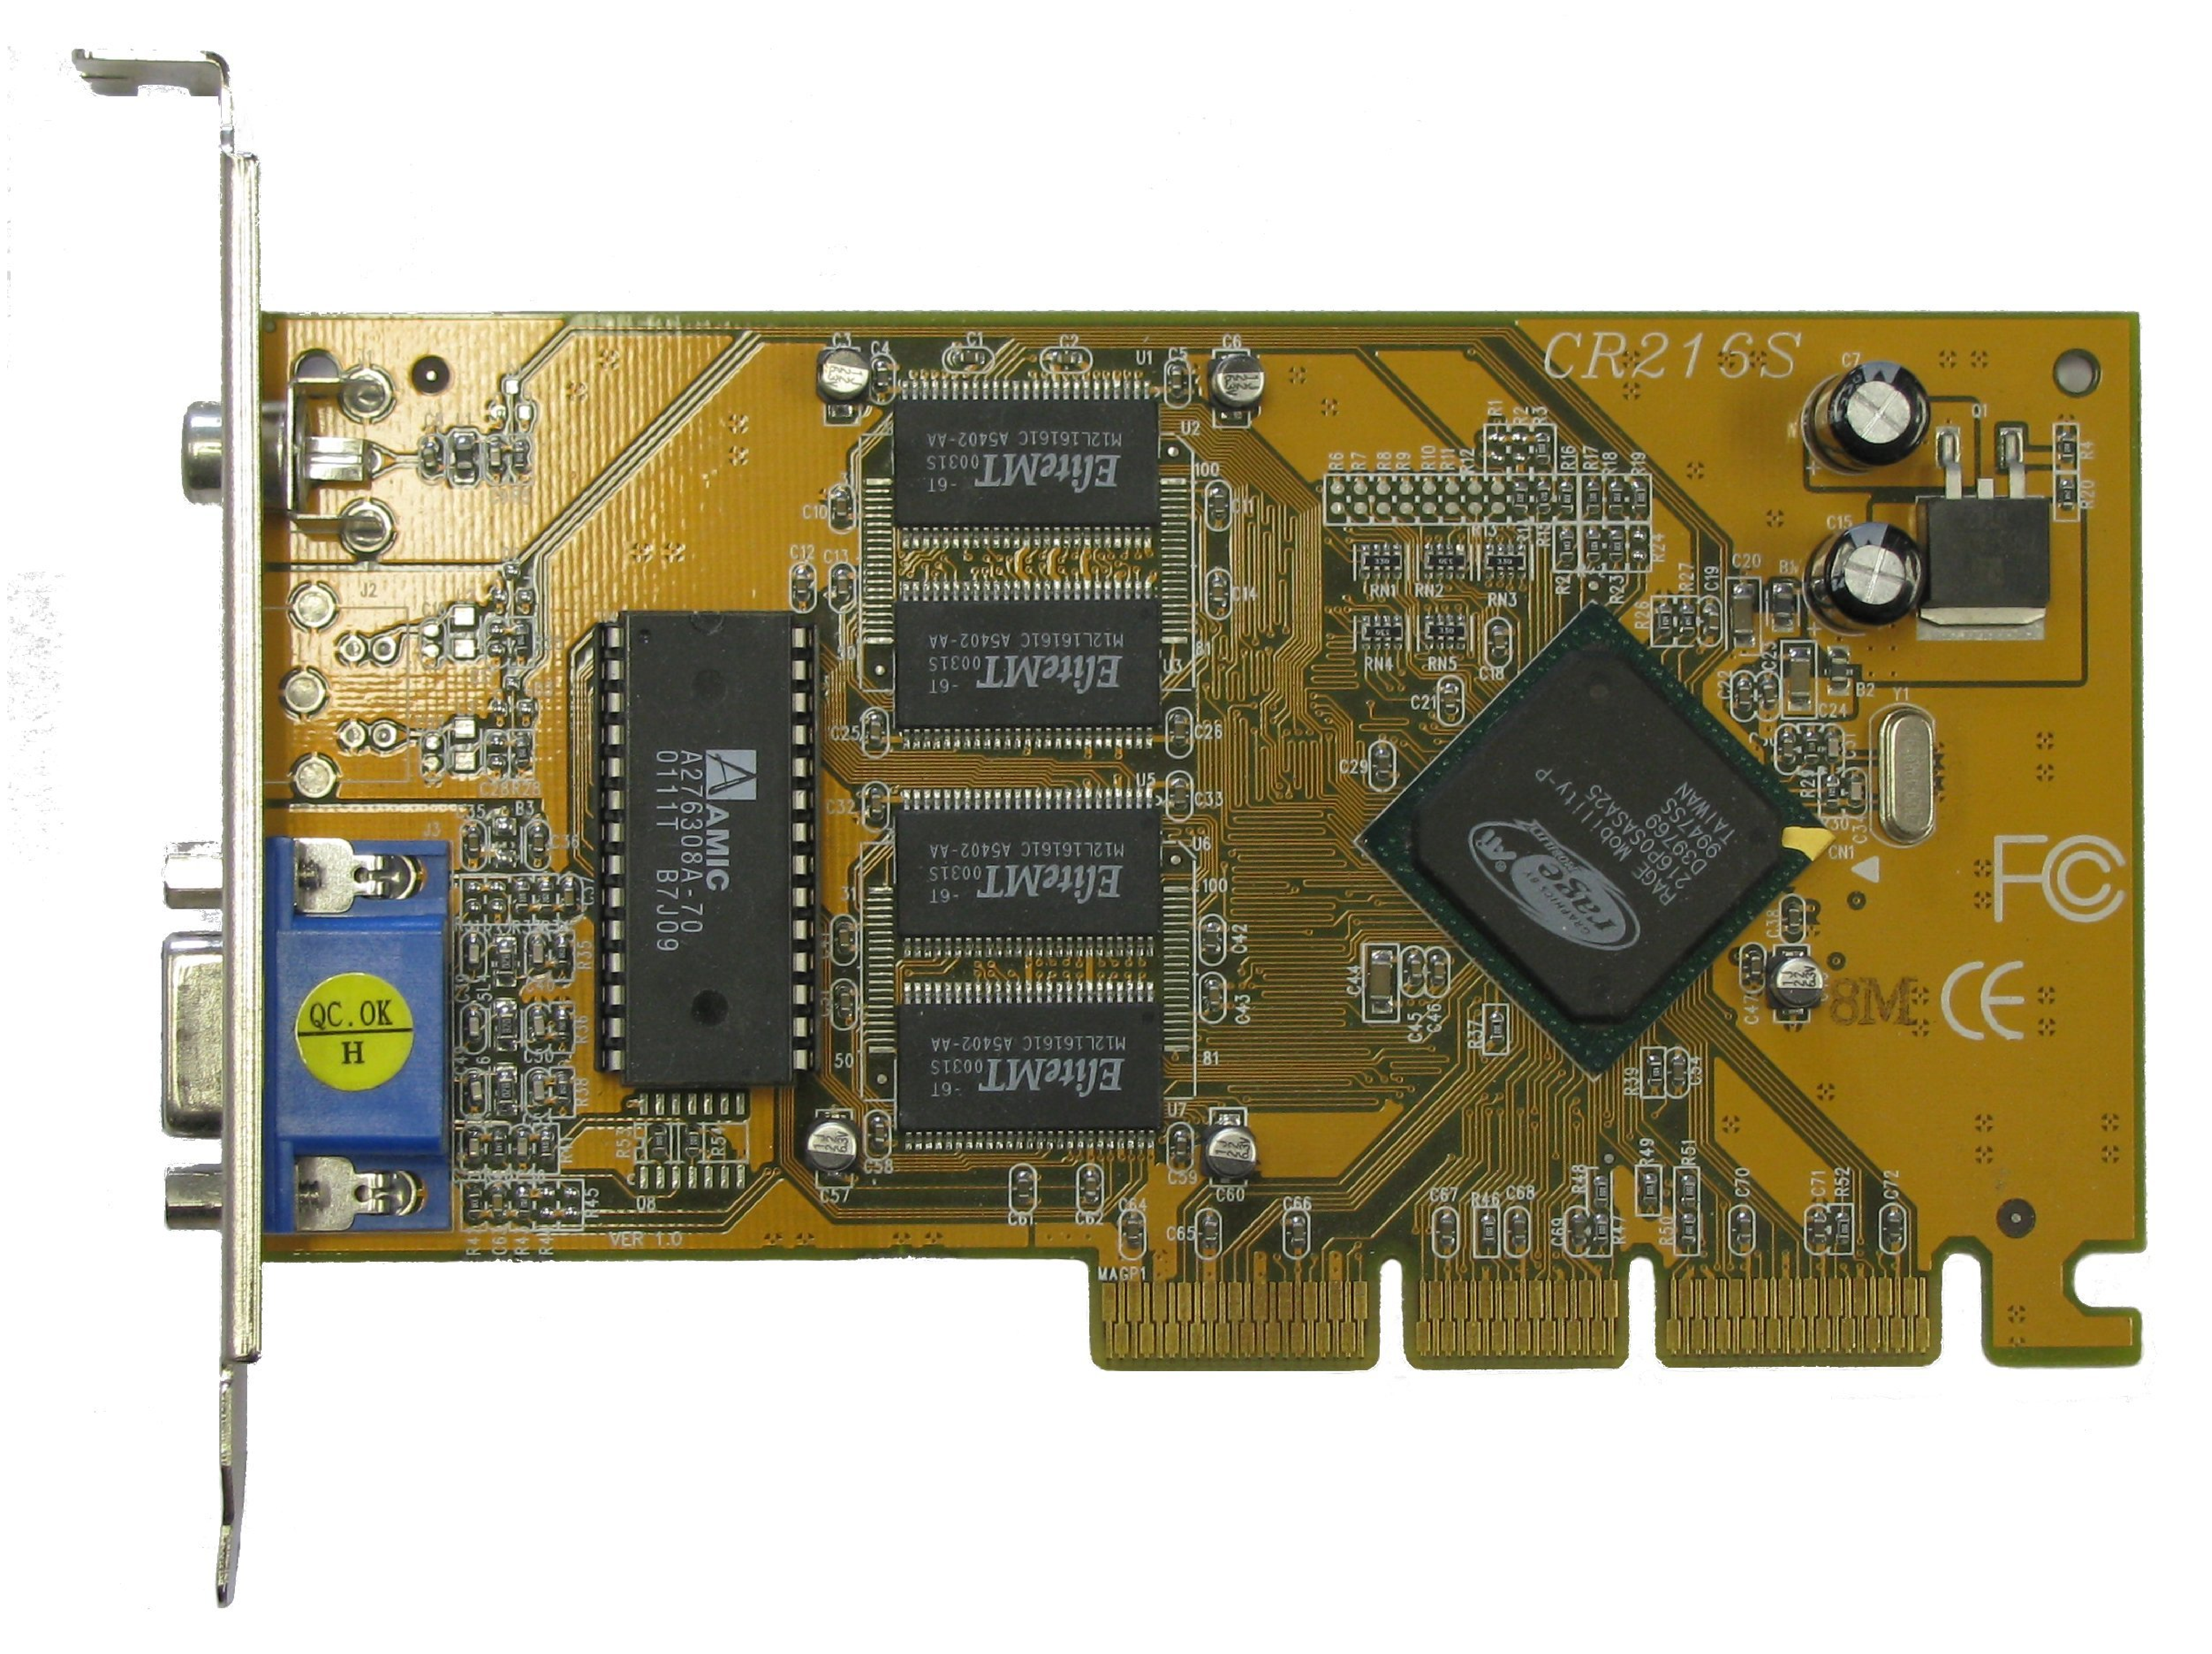
\includegraphics[width=\linewidth]{images/ati_rage.eps}
% convert -resize 1024 ati_rage.jpeg eps3:ati_rage.eps
\caption[ATi Rage graphics adpater]{ATi Rage graphics adapter with the
significant components identified.}
\end{center}
\label{INTRO_ATi_Rage}
\end{figure}


\section{PC Graphics Adapter History}
The original IBM PC featured a Monochrome Display Adapter\glossary{name={MDA},
description={Monochrome Display Adapter}} (MDA)~\cite{VGA_Programmers}. The MDA
only had a very small local memory due to the high cost of DRAMs. This memory
only stored ASCII (American Standard Code for Information
Interchange\glossary{name={ASCII}, description={American Standard Code for
Information Interchange}}, see Figure~\ref{INTRO_ASCII}) and attribute data for
several screenfuls of text (80 columns and 25 rows of ASCII characters). The MDA
had dedicated hardware which converted ASCII characters from text-buffer into
pixel values during display redraw periods. The pixel values were transmitted to
a monochrome CRT\glossary{name={CRT}, description={Cathode Ray Tube}} monitor for
display.

The original IBM PC was produced from readily available parts and was reverse
engineered by other companies to produce numerous compatible versions. This means
that the MDA had to be reverse engineered. Derivatives were produced that had
more features and were backwards compatible, like the Hercules graphics adapter
(sometimes called HGA).

The original IBM PC was the first in a line of computers, with future models
having different hardware, including changes to the display adapters. The later
graphics adapter standards: CGA, MCGA, EGA, VGA, 8514, XGA, and TIGA; all
followed MDA. These later adapters were reverse engineered and cloned as well,
though the display adapter standards after VGA never gained widespread
use~\cite{VGA_Programmers}.

VGA was extended by many manufacturers, increasing framebuffer sizes, numbers of
colours, higher resolution modes, and hardware acceleration for 2D and 3D
functions. The umbrella term for all of these adapters was Super
VGA\glossary{name={SVGA}, description={Super VGA}}, or SVGA. Every time a
different manufacturer produced a VGA compatible display adapter, they
essentially had to start from scratch, reimplementing VGA and adding their own
extensions. Some of these companies were: Oak, Advance, Genoa, NCR, Integrated
Info Tech, Tseng Labs, Weitek, Trident, Western Digital, Video7, VIA, SiS, Chips
and Technologies, Cirrus Logic, ATI, Nvidia, Intel, S3, and 3DFX.


\section{The Original IBM VGA}
The major components of a VGA-compatible graphics adapter are shown in
Figure~\ref{INTRO_ATi_Rage}. These components being: a VGA IC\footnote{The
earlier VGA adapters typically used separate ICs for the RAM DAC and the VGA, but
with this adapter, the functionality is combined into the main IC. Additionally,
this adapter contains hardware support for 3D graphics acceleration.}, some
memory for a framebuffer, a ROM containing the VGA BIOS, connector for
communicating with the host, connector(s) for attaching a display device, and
some power supply circuitry.


\subsection{The Video Graphics Array}
Before VGA, the graphics adapter's functional components were contained within
multiple ICs. VGA was IBM's first adapter which contained the majority of the
logic functionality within a single IC. The functions that were combined
into one ASIC were:

\begin{itemize}
  \item CRT controller
  \item Attribtue controller
  \item Sequencer
  \item Pixel data serialiser
  \item Graphics controller
  \item Miscellaneous control registers
  \item ASCII text to pixel converter
  \item Bus interface logic
  \item Memory controller
\end{itemize}


The CRT Controller\glossary{name={CRTC}, description={CRT Controller}} (CRTC)
generates the timing signals necessary to display an image on a VGA or DVI
connected monitor. Images are sent to a monitor as a stream of pixels, scanning
from left to right, and from top to bottom. The CRTC generates the signals which
synchronise the pixel-stream being sent. These are the horizontal
synchronisation\glossary{name={hsync}, description={Horizontal synchronisation}}
(hsync) signal that indicates the end of the current horizontal line, and the
vertical synchronisation\glossary{name={vsync}, description={Vertical
synchronisation}} signal that marks the end of the current screen (see
Figure~\ref{INTRO_CRT_Redraw} for more detail).

\begin{figure}[h!]
\begin{center}
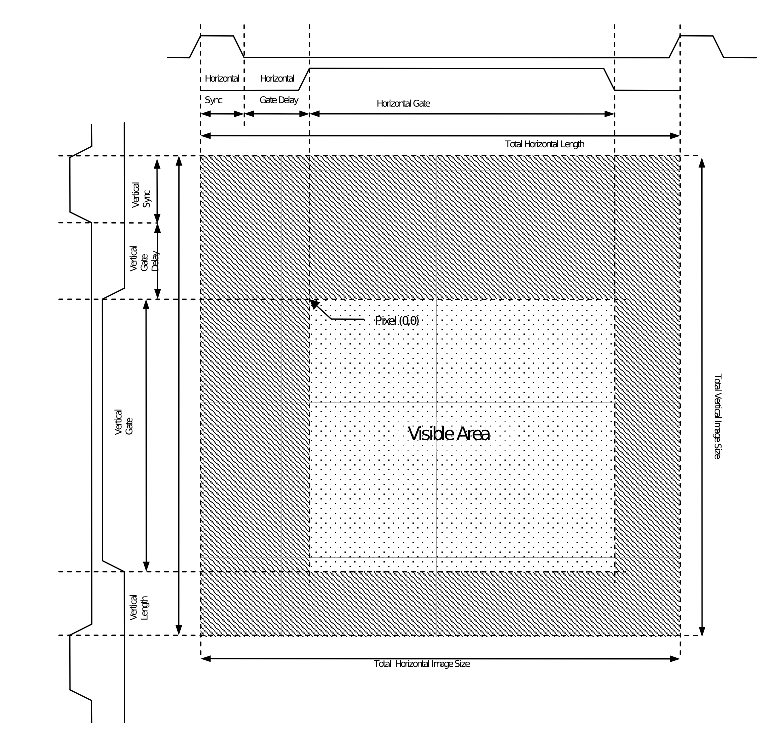
\includegraphics[width=0.9\linewidth]{images/crt_redraw.eps}
\end{center}
\caption[VGA display redraw timing and signals]{VGA display redraw timing and
signals. (Image from~\cite{knutsson:fbg}.)}
\label{INTRO_CRT_Redraw}
\end{figure}

Early VGA adapters, like their predecessors, had a very limited quantity of
framebuffer memory to store the image to be displayed, due to the price of DRAM
ICs. Rather than store every colour as RGB\glossary{name={RGB}, description={Red
Green Blue}} (Red Green Blue) components, the colours were stored as indices into
a colour palette. The palette contained the corresponding colour for a given
index, and the palette only contained indices for a subset of available colours.
This technique allowed the use of smaller framebuffers.

In monochrome modes, for example, one bit encodes the colour, so it can only be
one of two values. VGA supported 1-bit, 2-bit, 4-bit, and 8-bit colour modes. The
attribute controller was responsible for converting these colour indices into the
full 24-bit RGB colour format that the video DAC then converts to VGA compatible
analogue signals.

The attribute controller contains two colour look-up tables, or palettes, and
these are typically daisy-chained, the output of the first becoming the input to
the second (except in 8-bit, packed-pixel modes, where the first table was not
used). The first palette takes as input a 4-bit value and generates a 6-bit
value. This 6-bit value is combined with some additional register values, and is
used to generate the an 8-bit index into the second table. This 8-bit index into
the second palette retrieves an 18-bit output RGB value, 6-bits per colour
component, and is then combined with additional attribute controller registers to
extend it to the final 24-bit RGB format.

The attribute controller has other programmer accessible features too, it can
also mask pixels from any of the four bit-planes, depending on the video mode, can
enable pixel blinking, and can pan the display horizontally, which works in both
graphics and alphanumeric modes.

To set a single pixel, in the 4-bit colour mode for example, a single bit from
each of the four bit-planes (see the display memory explanation in
Section~\ref{VGA_Display_Memory}) may need to be modified, therefore each of the
four DRAMs needs to be accessed. To improve performance with these operations,
the graphics controller allows various programmer-set, bitwise operations and
shifts to be performed on the incoming data and combines these modified values
with the data stored in the bit-planes. Afterwards, the modified values are
written back to the DRAMs, and these operations are pipelined to achieve high
performance.

All of the timing signals required for the VGA are controlled by the sequencer,
and often generated from a single off-chip oscillator. The sequencer generated
dot-clock and character-clock signals control the timing for nearly all of the
VGA, with the exception of the external bus clock signal. One last feature of the
sequencer allows the bit-plane to be enabled or disabled too.

Pixel colour-values are not stored within the display memory when the VGA is
operating in alphanumeric modes. Only ASCII-encoded text along with its
corresponding attributes (see Figure~\ref{INTRO_ASCII} to see how ASCII
alphanumeric fonts were stored as bit-masks), and a font bit-mask, are stored in
the display memory. The attributes values for each ASCII character are foreground
and background text colour, and optionally a value that causes that particular
character to blink\footnote{Character blinking is achieved by periodically
swapping foreground and background colour as the character is decoded into
pixels.}. These alphanumeric modes were created since the memory storage
requirements are far lower than graphics modes where every pixel is addressable.
In the standard 80 column, 25 row, alphanumeric mode (from now on referred to as
80x25 text-mode), only requires 4 kB of DRAM. Due to the low memory requirements
of alphanumeric modes, up to eight ``pages'' were supported, and could be
dynamically exchanged by modifying user programmable registers.

\begin{figure}[h!]
\begin{center}
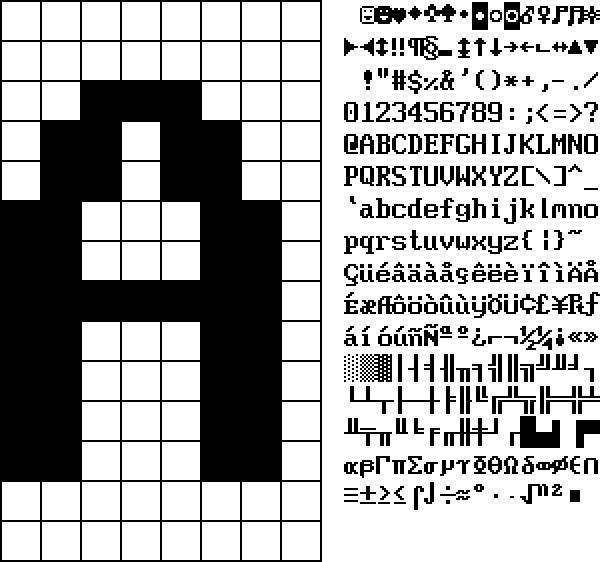
\includegraphics[width=\linewidth]{images/ascii.eps}
\caption[ASCII and extended-ASCII character set]{ASCII and extended-ASCII
character sets, and an example pixel representation.}
\label{INTRO_ASCII}
\end{center}
\end{figure}

VGA, and all earlier display adapters produced by IBM, includes dedicated
hardware for performing ASCII-character to pixel conversion, since it needs to
operate continuously while in alphanumeric modes. ASCII text is retrieved from
the framebuffer at the rate of the character clock, and converted to pixel data
at the rate of the dot-clock, which is 25.175 MHz in the default VGA 80x25
text-mode. The default VGA text-mode resolution is 640x400 pixels, with a redraw
rate of 60 Hz, and for the system's x86 processor (the generic name for the Intel
8086 CPU architecture and derivatives)\glossary{name={x86}, description={The
general name for a computer architecture based upon the Intel 8086 architecture
and derivatives}} to produce pixel values at this rate would have been difficult
in 1987 .

\begin{table}[h!]
\begin{center}
\begin{tabular}{c | c l}
Port & Direction & Register Description \\
\hline
3B4h & R/W & CRTC Controller Address Register \\
3B5h & R/W & CRTC Controller Data Register \\
3BAh & Read & Input Status $\#1$ Register \\
3BAh & Write & Feature Control Register \\
3C0h & R/W & Attribute Address/Data Register \\
3C1h & R/W & Attribute Data Read Register \\
3C2h & Read & Input Status $\#0$ Register \\
3C2h & Write & Miscellaneous Output Register \\
3C4h & R/W & Sequencer Address Register \\
3C5h & R/W & Sequencer Data Register \\
3C7h & Read & DAC State Register \\
3C7h & Write & DAC Address Read Mode Register \\
3C8h & R/W & DAC Address Write Mode Register \\
3C9h & R/W & DAC Data Register \\
3CAh & Read & Feature Control Register \\
3CCh & Read & Miscellaneous Output Register \\
3CEh & R/W & Graphics Controller Address Register \\
3CFh & R/W & Graphics Controller Data Register \\
3D4h & R/W & CRTC Controller Address Register \\
3D5h & R/W & CRTC Controller Data Register \\
3DAh & Read & Input Status $\#1$ Register \\
3DAh & Write & Feature Control Register \\
\end{tabular}
\end{center}
\caption[VGA I/O Ports]{VGA I/O Ports.}
\label{PCI_VGA_Port_Table}
\end{table}

All of the control registers of VGA were mapped to x86 I/O ports and these are
listed in Table~\ref{PCI_VGA_Port_Table}. For a device to be VGA-compatible,
these control registers have to be emulated. These registers were extended by
SVGA to allow more video modes, but these were not standardised between
manufacturers. Subsequently, directly programming SVGA registers is complicated,
but there are books which detail the programming of the more popular SVGA
graphics cards~\cite{SVGA_Book, VGA_Programmers}.


\subsection{Video DAC}
The video DAC converts 24-bit, RGB-encoded, colour values into the analogue
signals required to drive a VGA display. The video DAC was originally a
separate IC~\cite{VGA_Programmers, SVGA_Book} though modern graphics adapters
can include them within the main ASIC (see Figure~\ref{INTRO_ATi_Rage}). The
digital encoding consists of three 8-bit fields, representing each RGB colour
component, and the DAC produces analogue values which range in magnitude between
0.7 and 1.4 V.


\subsection{VGA BIOS}
Each VGA device requires a VGA Basic Input/Output System\glossary{name={BIOS},
description={Basic Input/Output System}} (BIOS)) ROM. This is a collection of
routines for performing video functions. These routines are accessed on an x86 PC
architecture by using software interrupts (using the instruction `int 10h',
register values are used as the arguments)~\cite{VGA_Programmers, SVGA_Book}, and
are typically written in just 16-bit, Intel 8086, assembly code.

The VGA BIOS contains routines for changing modes, setting pixels, cursor
positioning, and many others. These routines are required for VGA compatibility.
A separate ROM IC containing this code is usually present on a VGA board, as
shown in Figure~\ref{INTRO_ATi_Rage}. A free and open source implementation of
the VGA BIOS is available, and this is included within the OpenVGA project since
it provides all the required functionality, complete with a VESA BIOS Extensions
(VBE) implementation.


\subsection{Display Memory}
\label{VGA_Display_Memory}
The original IBM VGA had display memory that consisted of four 8-bit DRAMs, and
each DRAM contained the data for one of the four bit-planes (except in
packed-pixel modes, where the memory was not arranged as planes). The total
quantity of display memory on original VGA adapters was typically 256 kB, though
versions were available with only 64 kB or 128 kB of DRAM and could not support
all video modes. The portion of display memory which is involved with redrawing
the screen in the current mode is also called the framebuffer, as it stores
(buffers) the data for the current frame.

A VGA display adapter has graphics modes, which are also called ``all points
addressable'' modes, in which every pixel is mapped to a location in memory (or
multiple ``bit-planes'' in some VGA modes). For the 640x480 resolution graphics
mode, the maximum resolution officially supported by the original IBM VGA, there
are 307,200 pixels, each can be set individually. Some graphics modes support
multiple pages of image data. These can be exchanged, typically during the
vertical-synchronisation period, to achieve a smooth animation effect.


\section{Non-VGA Graphics Adapters}
Graphics adapters have been developed and produced that are designed to be
installed and used alongside a VGA adapter within a PC. Prominent examples are a
couple of the 3D graphics accelerators produced in the 1990s, the PowerVR Series
1, and 3DFX Voodoo Graphics (later referred to as Voodoo 1) and Voodoo 2. The
primary graphics adapter, typically a SVGA, is used for all 2D modes, like those
commonly used by OS Graphical User Interfaces\glossary{name={GUI},
description={Graphical User Interface}} (GUIs). Once a 3D application is started,
like a computer game, the 3D graphics accelerator is activated and is used to
redraw the display instead.

The PowerVR and Voodoo 1 \& 2 adapters used a pass-through architecture, where
the primary graphics adapter had its output redirected to the 3D accelerator, in
a daisy-chain configuration. This was achieved with a short ``loopback'' cable
routed from the primary adapter to the input port of the secondary adapter. The
output of the secondary adapter was connected to the display device, typically a
SVGA CRT monitor.


\section{Related Projects}
There exists several other graphics adapter projects, and a brief overview of
these is given. The most extensive of these is the Open Graphics Project, with
aims to produce both FPGA and ASIC graphics adapters, and including support for
multiple operating systems. Also planned is 3D acceleration, including support
for OpenGL~\cite{OpenGL}\glossary{name={OpenGL}, description={The Open Graphics
Library}}, an open-specification 3D graphics library.


\subsection{Open Graphics Project}

\begin{figure}[h!]
\begin{center}
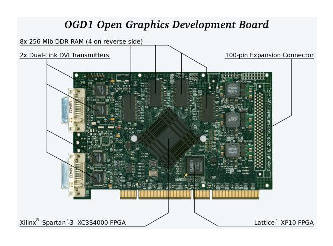
\includegraphics[width=\linewidth]{images/ogd1_showcase.eps}
\end{center}
\caption[OpenGraphics OGD1]{OpenGraphics OGD1 PCB and components. (Image
from~\cite{OpenGraphics}.)}
\label{INTRO_OGD1}
\end{figure}

Open Graphics Project\footnote{For more information see http://opengraphics.org/}
is a prominent open-source VGA project, which aims to develop a VGA compatible
display adapter with hardware 3D acceleration support, and OpenGL drivers.
Development is currently using an FPGA-based board, called OGD1 (See
Figure~\ref{INTRO_OGD1}), but the project's stated goal is to raise enough money
to have an ASIC fabricated.

OpenGraphics has an impressive feature list, allowing for a very capable graphics
adapter, and is significantly more complex than what was planned for OpenVGA, but
the cost of the development boards is around 1000 USD. Their plan is to emulate
VGA using a soft processor core. The OGP processor core is a 32-bit RISC design,
and the architecture is similar to a MIPS processor~\cite{OpenGraphics}.

The OpenGraphics source code is freely available and licensed under the GPL, but
all contributions back to the project require copyright be assigned to Traversal
Technologies Incorporated so they can dual-license the code to sell commercial
versions of it.

At the time of writing this, the development of OGP has reached the point where
they have OGD1 running as a simple non-VGA framebuffer device, and now can run
code on their soft-processor core too.


\subsection{Project VGA}

% \begin{figure}[h!]
% \begin{center}
% 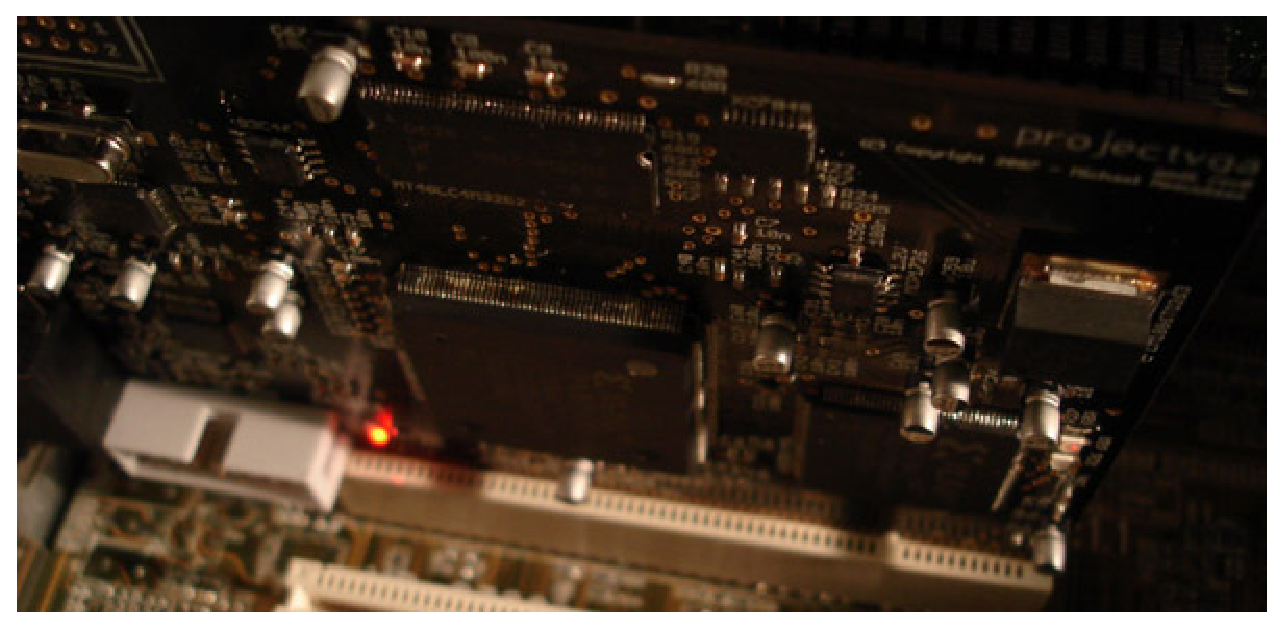
\includegraphics[width=\linewidth]{images/project_vga.eps}
% \end{center}
% \caption[Project VGA Photograph]{Project VGA promotional photograph.
% \textit{Image obtained from http://wacco.mveas.com/}}
% \label{INTRO_ProjectVGA}
% \end{figure}

This project has stated aims similar to OpenVGA, it aims to be low-cost, simple,
VGA compatible, open-source graphics adapter (see http://wacco.mveas.com/).
Unfortunately though, the status of this project does not appear to have been
updated since 28/02/08 .


\subsection{Manticore}
The goal of this project was to develop a non-VGA, 3D graphics accelerator, and
once this stage was complete, add 2D support to it. The project uses an older model
Altera FPGA and does not seem to have been updated in the last three years.

\chapter{OpenVGA Outline}
\label{OPENVGA}

This chapter presents an introduction to the architecture of the OpenVGA graphics
adapter that was developed for this thesis. OpenVGA has 8 MB of local memory
which stores pixel colour information, firmware code, and state information. This
memory is accessible to the host computer so it can modify the contents of the
framebuffer and firmware. OpenVGA continuously encodes and transmits frames of
pixel data to the computer monitor that is connected to it, typically at 60
frames per second.

An outline of the OpenVGA hardware, HDL logic-cores, firmware, and software
drivers are covered here. Figure~\ref{OPENVGA_OpenVGA} introduces OpenVGA
hardware and Figure~\ref{OPENVGA_Arch} is an architecture-overview block diagram
that contains the components which will be discussed within this chapter. Many of
these components will be further elaborated on in the following chapters.

\begin{figure}[h!]
\begin{center}
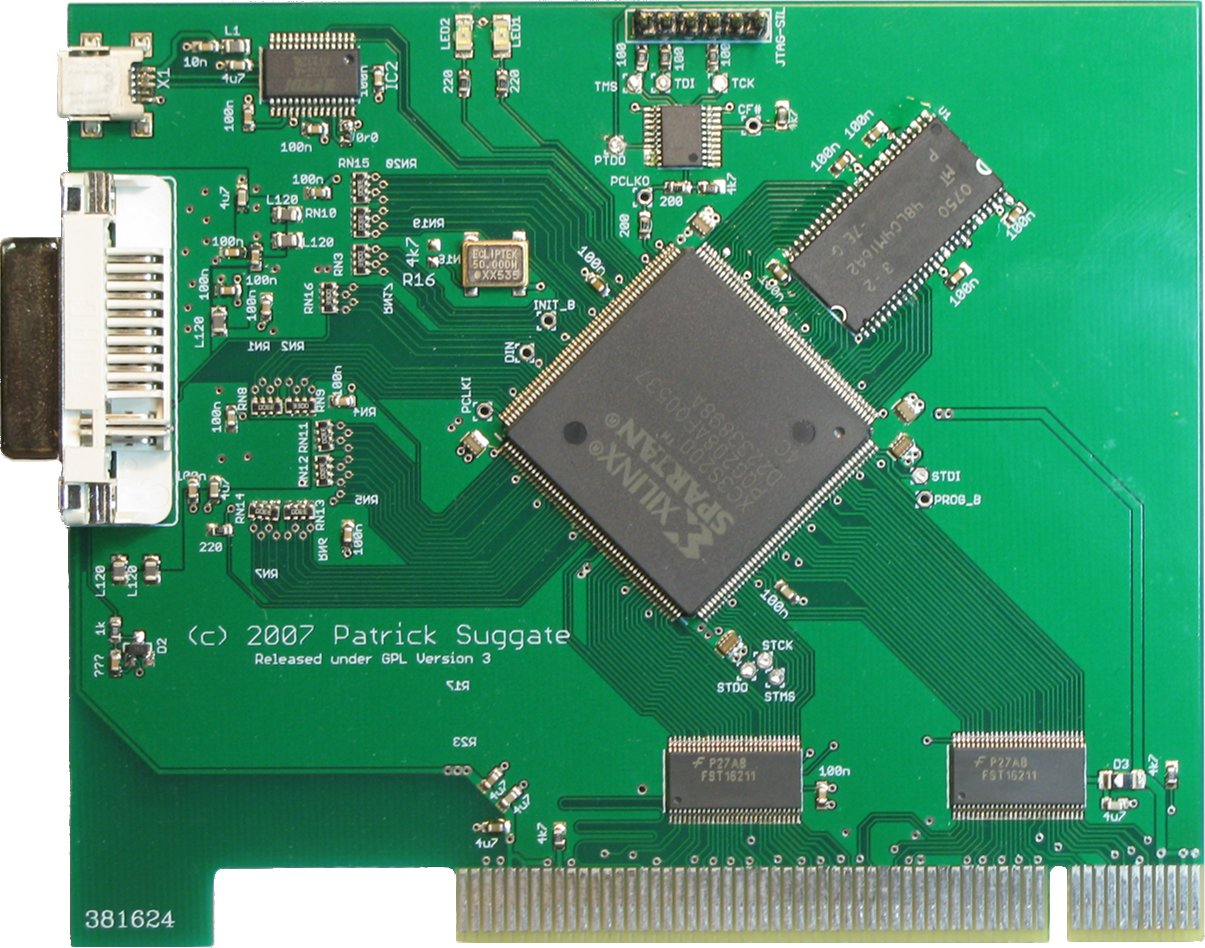
\includegraphics[width=\linewidth]{images/freega_overview.eps}
\caption[OpenVGA Hardware Features]{OpenVGA Hardware Features.}
\label{OPENVGA_OpenVGA}
\end{center}
\end{figure}


\section{Hardware Development}
\label{OPENVGA_Hardware}

Most of the significant hardware components of OpenVGA are shown in
Figure~\ref{OPENVGA_OpenVGA}. Components not shown in this image are the VGA
video DAC\glossary{name={DAC}, description={Digital to Analogue Converter}} and
the DVI TMDS encoder, as these components are soldered to the reverse side of the
PCB (see Figure~\ref{HARD_Bot}). The PCB only has two copper layers to meet two
of the design goals of OpenVGA, simplicity and low-cost. A full list of all of
OpenVGA's electronic components and where to obtain the PCB artwork is found in
Appendix~\ref{HARDWARE}.

Logic cores were developed which interface to many of these hardware components.
There are logic cores implementing functionality for PCI, controlling the Video
RAM, sending and receiving via the USB UART, and encoding video data for either
DVI or VGA displays. These logic cores are introduced later in this chapter in
Section~\ref{OPENVGA_Logic_Cores}.

\begin{figure}[h]
\begin{center}
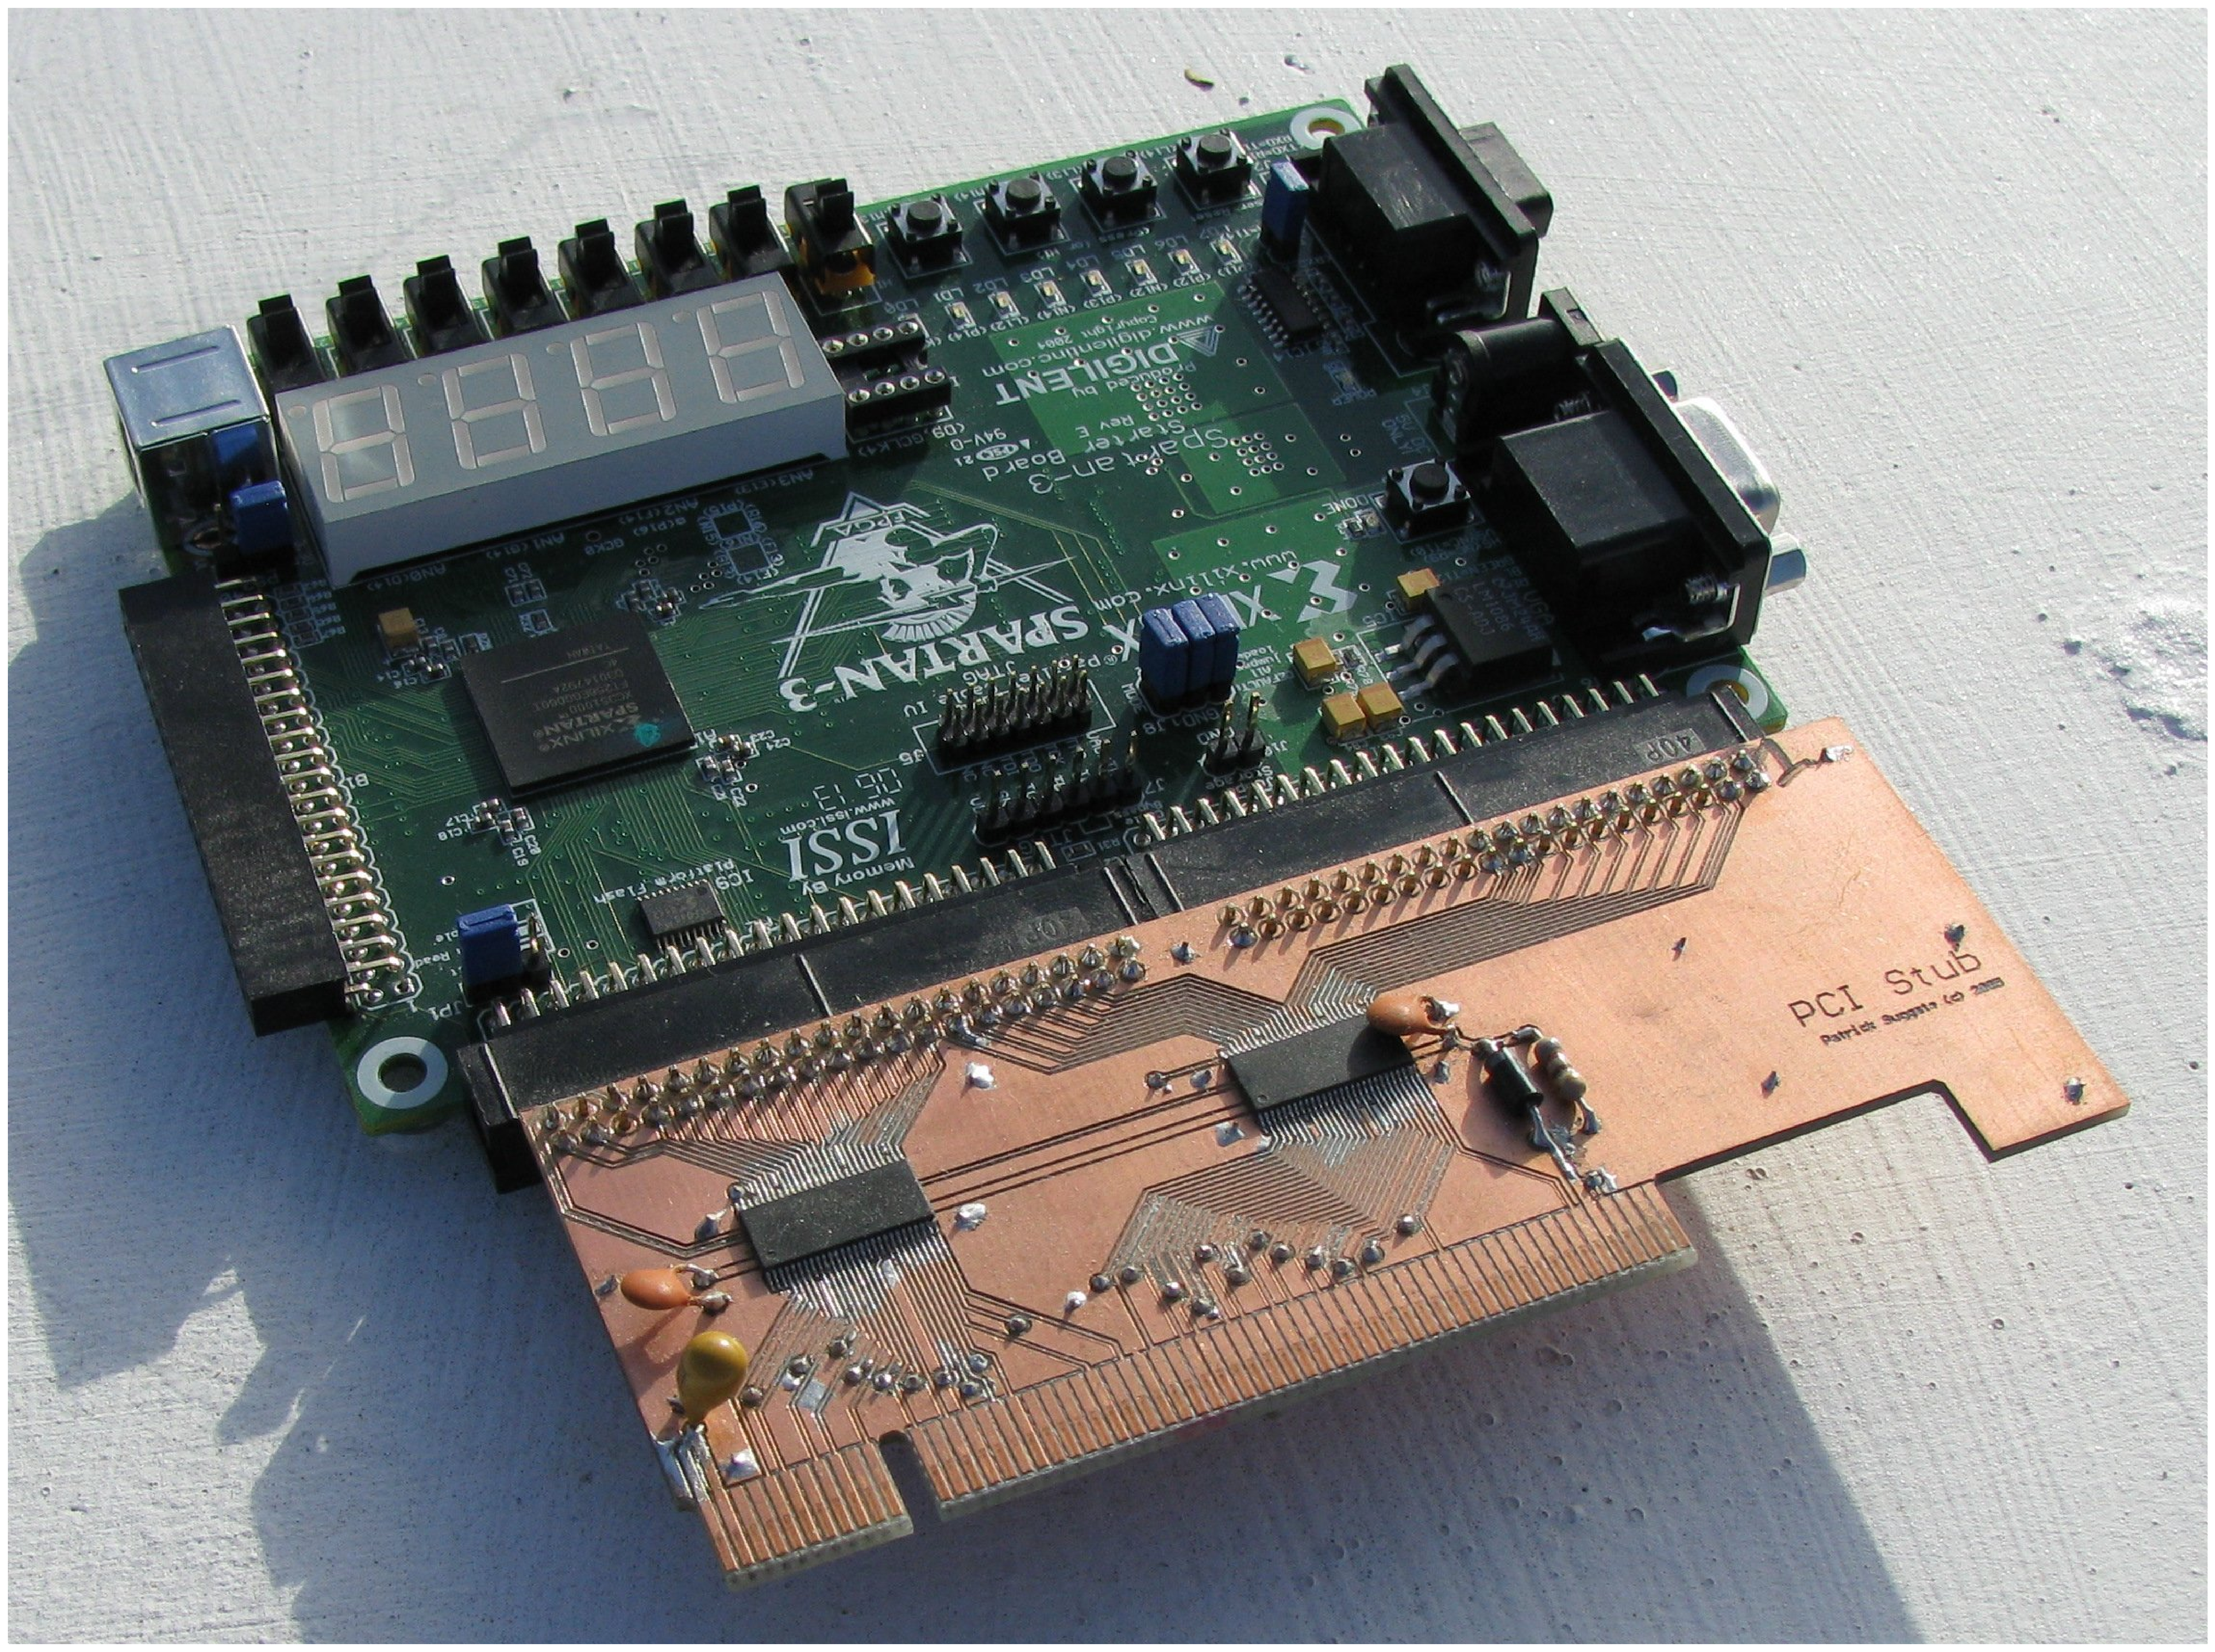
\includegraphics[width=\linewidth]{images/pci_stub.eps}
\caption[PCI development stub board]{PCI development stub board. The
bus-switches, which are visible in the middle of the copper coloured PCB,
translate the PCI's 5 V signals to the 3.3 V required by the Spartan-3 FPGA.}
\label{OPENVGA_PCI_Stub}
\end{center}
\end{figure}

Initial hardware development concentrated on adding PCI support to an existing
Spartan-3 development board, as shown in Figure~\ref{OPENVGA_PCI_Stub}. The PCI
logic core needed to be developed first as this allowed the host PC to run
testbenches on the logic cores which were developed later. A simple PCI stub PCB
had to be constructed (the copper-coloured board shown in the photograph). This
board contains only two ICs, just simple bus-switches to translate between the
3.3 V signalling of the Spartan-3 development board and the 5 V PCI signalling
used in many PCs.

The stub board was then connected to a commercial Spartan-3 Starter Kit
development board (the green circuit board shown in the photograph) to develop
the PCI-to-Wishbone-bridge logic core (see Sections~\ref{OPENVGA_PCI}
and~\ref{PCI}). An additional advantage of this arrangement was that the
connectors between the stub board and the development board allowed digital
oscilloscope probes to be attached. This made debugging of the PCI logic core
easier since the electrical signals of the PCI bus could be monitored during
testing (see Figure~\ref{PCI_CFG_Cap}).

\begin{figure}[h]
\begin{center}
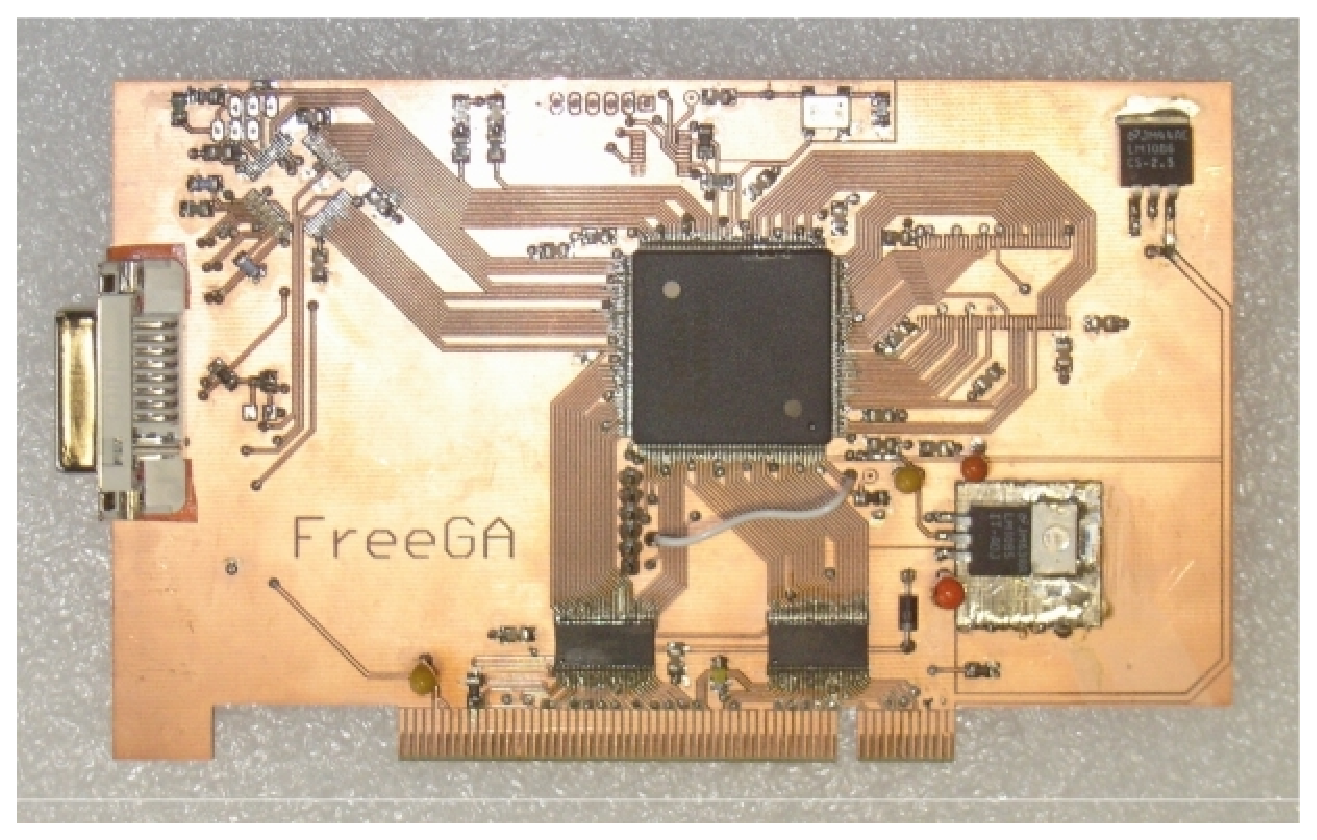
\includegraphics[width=\linewidth]{images/FreeGA_orig.eps}
\caption[OpenVGA PCB version 2 with DDR SDRAM]{Prototype PCB featuring DDR
SDRAM, DVI, and only eight colour VGA (via the DVI analogue outputs).}
\label{OPENVGA_Version2}
\end{center}
\end{figure}

Following this, an initial prototype board for OpenVGA was milled in-house, on a
LPKF\texttrademark~PCB milling machine, and is shown in
Figure~\ref{OPENVGA_Version2}. This board was an attempt to use Double Data
Rate\glossary{name={DDR}, description={Double Data Rate}} (DDR) SDRAM with
OpenVGA to provide greater memory bandwidth\footnote{The DDR SDRAM specification
requires that signal traces be terminated, since DDR SDRAM was designed to
operate at frequencies up to 200 MHz. The OpenVGA DDR version of the PCB did not
allow for these resistors since satisfactory placement would be extremely
difficult with the two-layer PCB used, since there are no ground-planes. It was
decided to attempt DDR support without termination resistors, since the
trace-lengths were very short, but DDR SDRAM could not be made to operate.}.
Though the DDR SDRAM controller was successfully simulated with the Icarus
Verilog simulator, using the Micron-provided DDR SDRAM Verilog module, the
synthesised design did not work\footnote{The DDR signals showed significant
overshoot and undershoot when monitored on an oscilloscope, and the DDR IC
produced a lot of heat.}. Due to the problems with DDR SDRAM, the final version
of the OpenVGA PCB was designed to use standard, single data-rate SDRAM (labelled
as ``Video RAM'' in Figure~\ref{OPENVGA_OpenVGA}).


\section{Important Design Elements within the FPGA}
\label{OPENVGA_Logic_Cores}
Implemented within OpenVGA's Spartan-3 FPGA are many logic cores and the
necessary bus and clocking logic. Figure~\ref{OPENVGA_Arch} shows the significant
features of the digital-logic design, and the FPGA's connectivity with the other
on-board components of OpenVGA. All logic was described using the Verilog HDL,
simulated using Icarus Verilog, and synthesised using tools which Xilinx freely
provides for use with their FPGAs.

The design contains a processor core for data processing, initialisation, and
mode-managing tasks. OpenVGA can be configured to be use either one of the two
processors that were developed for this project, TTA16 or RISC16. Additional
cores are a small data cache since memory latency is high, a SDRAM controller, a
PCI-to-Wishbone bridge, logic to read the SPROM\glossary{name={SPROM},
description={Serial Programmable Read Only Memory}} (Serial Programmable ROM),
and numerous other support modules.

\begin{figure}[h!]
\begin{center}
\includegraphics[width=\linewidth]{images/freega_arch.eps}
\caption[OpenVGA Architecture Block Diagram]{OpenVGA Architecture Block Diagram.}
\label{OPENVGA_Arch}
\end{center}
\end{figure}


\subsection{Logic Core Interconnection}
The Wishbone interconnect standard\footnote{Wishbone is called an
``interconnect'', instead of a ``bus'', standard as it allows for numerous
circuit topologies: buses, crossbar switches, point-to-point, and many others.}
was used as the standard interface for communication between logic cores. This
standard was designed for System-on-a-Chip\glossary{name={SoC},
description={System-on-a-Chip}} (SoC) applications, is very flexible, is commonly
used with other open-source hardware projects, and requires very little logic to
implement. Appendix~\ref{APP_Wishbone} gives a brief introduction to Wishbone,
covering the core signals and providing a simple example implementation.


\subsection{FPGA-Optimised Processor Cores}
The OpenVGA initialisation, state-management, and data-processing tasks were to
be performed using a processor logic core. Existing processor logic cores were
considered but, due to performance, capability, and size requirements, two new
processors were developed for OpenVGA instead. OpenVGA requires a processor that
is be able to address at least 8 MB of memory, so this ruled out existing 8-bit
processors. The evaluated 32-bit processors were too large, so a fast 16-bit
processor was needed, but nothing suitable was found.

The first processor developed was a novel TTA processor. Significant research has
been done with this class of architecture~\cite{corporaal1993maa,
jaaskelainen2007cta}, but there are very few commercial processors of this type.
The second is a more traditional Reduced Instruction Set
Computer\glossary{name={RISC}, description={Reduced Instruction Set Computer}}
(RISC) architecture processor design. It was developed to compare with TTA16, the
first OpenVGA processor. Optimised for the same tasks, both processors used the
similar functional units. This provides a good platform for the comparison of
these two architectures.


\subsubsection{TTA16}
TTA16 is a 16-bit, Wishbone-compatible, TTA processor that can operate at up to
190 MHz, and has a very small footprint\footnote{These results are for synthesis
on a Spartan-3 FPGA, and depend on the build configuration and synthesiser
optimisation settings.}. It has a fixed, 32-bit instruction word and can perform
four data transports every clock cycle. This processor is covered in detail in
Section~\ref{TTA16}, and Appendix~\ref{TTA_Programming} is a programming guide
for TTA16.


\subsubsection{RISC16}
Due to the difficulty of writing assembly code for TTA16, RISC16 was developed
and is of a more traditional design. While not as fast as TTA16, operating at up
to 140 MHz, instruction width is only 16-bits so code density is better. The
external interface is Wishbone-compatible too, and is therefore identical to
TTA16, so that this logic core can be a drop-in replacement. More detail of
RISC16 is within Section~\ref{RISC16}, and Appendix~\ref{RISCPROG} is a simple
programming guide.


\subsection{Processor Data Cache}
A low-latency, Wishbone-compatible, data cache was needed for adequate processor
memory-access performance. The 8 MB of on board memory is shared amongst multiple
logic cores, and the latency is several Wishbone cycles, so any processor access
would lead to stalls of many cycles. Both interfaces to this cache are Wishbone,
and the number of width memory-address bus is parameterisable.

Other cache features are a fast-hit path with a latency of zero cycles, a slower
hit path of one cycle of latency, operating frequency of 150 MHz, two-way
set-associativity, a line-size of 64 bytes, and a capacity of 2 kB. A full
explanation of the cache's features and design decisions is within
Section~\ref{MEM_Cache}).


\subsection{Clock Domains and Domain Crossing}
OpenVGA has multiple external interfaces and several different and asynchronous
clocks. OpenVGA has three clock domains, these are the 50~MHz Wishbone bus
domain, the 33~MHz PCI Local Bus domain, and the dot-clock domain. While the PCI
bus typically operates at a frequency of 33 MHz, though this is not guaranteed,
and this clock signal is driven by the system host. The dot-clock of display
circuitry depends upon the video mode, as higher resolutions require more pixels
be drawn, therefore requiring a higher pixel rate. Currently the dot-clock can be
selected as either 25 MHz or 40 MHz (see Section~\ref{VIDEO_Modes}).

As well as asynchronous clock domains, some components of OpenVGA run at integer
multiples of the Wishbone domain's 50 MHz clock rate, the SDRAM and RISC16
operate at 100 MHz, and TTA16 operates at 150 MHz. These clocks are synchronous
with the Wishbone clock and present fewer problems. A further explanation and
solutions are covered in Section~\ref{CLOCK_Sync}.

When logic cores have different clocks, data must be synchronised when passing
from one core to the other. When the clocks are asynchronous this becomes even
more difficult due to metastability issues. A D-type
Flip-Flop\glossary{name={DFF}, description={D-type Flip-Flop}} (DFF) can enter a
metastable state\footnote{This metastable state means that the output of the DFF
is essentially random, but it oscillates for a significant time before it settles
back into a stable state~\cite{Async_FIFO2}.} when setup and/or hold times are
violated. Section~\ref{CLOCK} presents the OpenVGA clock architecture and
domains, examines the problems with domain crossing, and presents the solutions
used to solve these. Asynchronous First-In, First-Out
queues\glossary{name={FIFO}, description={First-In, First-Out queue}} FIFOs allow
signals that are multiple bits wide to be synchronised across clock domains and
are presented in Section~\ref{CLOCK_Async_FIFO}.


\subsection{Memory Controller}
\label{OPENVGA_Mem_Ctrl}
A high performance, small logic foot-print, Wishbone-compatible memory controller
was needed for OpenVGA. Tasks the controller has to perform include refreshing
the DRAM, support burst reads and writes, and atomic reads and writes. To
minimise the size of the controller it has to operate within the Wishbone clock
domain so that asynchronous FIFOs are not needed.

The SDRAM data transfers occur at 100 MHz while the controller's state machine
operates at 50 MHz, the Wishbone memory bus frequency. This was achieved by using
the DDR input and output primitives within the Spartan-3 I/O
Blocks\glossary{name={IOB}, description={Input/Output Block}} (IOBs).
Section~\ref{MEM_SDRAM} provides more detail on the controller, including the
design of the state machine and data path implementations.


\subsection{PCI-to-Wishbone Bridge}
\label{OPENVGA_PCI}
A small PCI-to-Wishbone-bridge logic core was developed so that the system host
can communicate with OpenVGA. This bridge supports the ``Plug and Play'' standard
and Memory-mapped I/O\glossary{name={MMIO}, description={Memory-Mapped
Input/Output}} (MMIO), which maps the OpenVGA SDRAM into the host PC's memory
address space. Only the PCI Local Bus features that were needed for OpenVGA are
implemented and resulted in a design about one-tenth the size of another
available open-source PCI bridge\footnote{There is a very capable, FPGA-tested,
PCI bridge available over the Internet from OpenCores site.}. The design of the
bridge, descriptions of its state-machines, and domain crossing issues are
explained Section~\ref{PCI}, and more details of the clock domain issues are
covered in Section~\ref{CLOCK}.

So that the host OS can access OpenVGA, a simple Linux kernel module was written.
Linux kernel modules are written using the C programming language\footnote{A
comprehensive guide to developing Linux kernel modules is available
from~\cite{salzman:lkm}.} and OpenVGA is accessed from the GNU/Linux OS by
opening the device file which represents the MMIO of OpenVGA. Using read, write,
and seek operations, any location within the OpenVGA SDRAM can be read and
written.


\subsection{VGA/LCD Display Controller}
This logic core prefetches image data from the memory controller, using the
system's memory Wishbone bus, and generates the timing signals and bit-streams
necessary for driving VGA and LCD displays (see Section~\ref{VIDEO}). The
Wishbone bus can be in a different clock domain to the dot-clock since an
asynchronous FIFO is used for the prefetch logic. This has a 2 kB prefetch
capability and is discussed in more detail in Section~\ref{VID_Prefetch}.

Within the display controller is a CRT controller which has registers that can be
accessed using a Wishbone interface. This allows the timing parameters to be set
allowing the display mode to be changed (see Section~\ref{VID_CRTC}).


\subsection{Additional Logic Cores}
Other smaller logic cores were developed for OpenVGA. Detailed explanations of
these can be found within Chapters~\ref{MEM} (Memory) and~\ref{IO_Chapter}
(I/O), and a summary of these is:

\begin{itemize}
  \item USB UART: A Wishbone-compatible interface to a 9600 baud UART which
  communicates with the on-board FTDI FT232R USB UART IC. More detail can be
  found in Section~\ref{USB_Sport}.
  \item LED driver: There are two Wishbone-mapped LEDs that can be set and
  cleared using this module, covered further in Section~\ref{LED_Driver}.
  \item DMA controller: A simple Direct Memory Access controller is used to
  improve the memory write performance of OpenVGA's processor. This logic core
  is detailed in~\ref{MEM_DMA} and a programming guide for it is in
  Appendix~\ref{TTAPROG_DMA}.
  \item Serial PROM reader: Spartan-3 FPGAs require configuration upon
  power-on. The on-board serial PROM contains this configuration data but also
  has enough capacity to store some extra data. This module can read this data
  from the SPROM when requested via its Wishbone interface.
  Section~\ref{Serial_PROM} presents more information on this module.
\end{itemize}


% Three chapters on the internal architecture.
\chapter{The TTA16 and RISC16 Processor Cores}
\label{CPU}

OpenVGA is designed to use a processor logic core for initialisation, mode
setting, and data processing tasks. Two processors were developed for these
tasks, the first was TTA16, a novel, 16-bit, transport-triggered processor. The
second processor that was developed, RISC16, a 16-bit, RISC processor
architecture, was for comparison with TTA16, and for its relative ease of
programming in assembly language.


\section{Processor Architectures}
An aim for OpenVGA's processor was to be fast enough to emulate VGA text-mode.
After evaluating existing FPGA-based, processor logic cores (see
Table~\ref{SUMMARY_CPU_Table}), it was decided to develop a new processor to meet
this speed and size criteria. Popular Instruction Set
Architectures\glossary{name={ISA}, description={Instruction Set Architecture}}
(ISAs) were considered for the OpenVGA processor. These included Complex
Instruction Set Computer\glossary{name={CISC}, description={Complex Instruction
Set Computer}} (CISC), RISC, and Very Long Instruction Word\glossary{name={VLIW},
description={VHSIC (Very Long Instruction Word}} (VLIW) architectures.

Figure~\ref{CPU_Sched} gives a breakdown of the tasks that a compiler and
processor must perform, and the division of these tasks for differing processor
architectures. Modern superscalar CISC and RISC processors use a lot of die area
for functionality other than transporting and processing data. This often
includes hardware for instruction decoding, out-of-order execution, speculative
execution, and branch prediction~\cite{parhami2005cam}. TTA processors typically
do not have these features~\cite{corporaal:tta}, with most of the logic gates
used for data transports and Functional Units\glossary{name={FU},
description={Functional Unit}} (FUs), resulting in smaller processor designs.

\begin{figure}[h!]
\begin{center}
\includegraphics[width=\linewidth]{images/hardware_sched.pdf}
\caption[The division of responsibilities between hardware and compiler]{The
division of responsibilities between hardware and compiler. (Image
from~\cite{corporaal1999tmi})}
\label{CPU_Sched}
\end{center}
\end{figure}

An efficient architecture would operate at a high frequency, have a high FU
utilisation rate, and use minimal logic resources. FPGAs have reduced frequency
and fewer logic gates than similar generation ASICs so a smaller, faster
processor architecture is arguably even more important. This is why a TTA
processor was chosen for OpenVGA. But the complexity of generating efficient
firmware code for TTA16 is why a second processor, RISC16, was developed.

TTA processors were investigated (designed, built, programmed, and characterised)
at the Technical University of Delft by Henk Corporaal et.
al.~\cite{corporaal1999tmi, corporaal:tta, corporaal1993maa} during the 1990s.
Additional TTA research has focused on the automatic generation of the HDL
source-code for TTA processor logic cores~\cite{hoogerbrugge1995ast,
jaaskelainen2007cta}. The goal has been to develop application-specific
processors for certain tasks, like image processing
applications~\cite{corporaal1999tmi}.

Xilinx Spartan-3 FPGA logic resources, and their latencies, also affect the
choice of processor architecture, and which features can be implemented
efficiently as well. The Spartan-3 has 18-bit embedded multipliers, fast
carry-chain logic, 16-entry and 2~kB RAM primitives, DCMs (Digital Clock
Modules), and some additional multiplexing primitives\footnote{The high
combinatorial logic delays of multiplexers synthesised for Spartan-3 FPGAs
influenced many design decisions. Even with some hardware support for wide
multiplexers these were still quite slow~\cite{Xilinx_SP3_DS}.}. These available
FPGA resources influenced the architectures evaluated, and the design choices
made.

Both of the processor logic cores developed for OpenVGA, TTA16 and RISC16,
feature a data word-size of 16-bits for two main reasons:
\begin{itemize}
  \item Functional units are typically half the size of those for 32-bit
  processors so the resulting processor will be a lot smaller.
  \item Wider signal paths use more routing resources, and are more difficult
  for the Xilinx PAR tool to route, usually resulting in lower frequencies.
\end{itemize}


\section{Shift Registers as Program Counters}
Rather than use a standard, base-2 incrementer for each processor's Program
Counter\glossary{name={PC}, description={Program Counter}} (PC), a Multiple
Feedback Shift Register\glossary{name={MFSR}, description={Multiple Feedback
Shift Register}} (MFSR)~\cite{MFSR_List} is used as the PC incrementer for both
TTA16 and RISC16. The count order of an MFSR is very different to standard base-2
incrementers. To illustrate this different increment sequence, an application of
MFSRs is for use as pseudo-random sequence generators. For a maximal-cycle MFSR
having $n$-bits, the cycle length is $2^n-1$, and can be implemented with a
maximum of just one layer of logic gates (see Figure~\ref{CPU_MFSR8}).

The reason for using MFSRs as PCs is due to the extremely small combinatorial
logic delay, just the propagation delay through one FPGA Look-Up
Table\glossary{name={LUT}, description={Look-Up Table}} (LUT) and some routing
fabric. This allows the PC increment and branch logic to have very low latency,
avoiding the requirement pipeline registers, or becoming the processor's critical
path and limiting maximum frequency.

\begin{figure}[h!]
\begin{center}
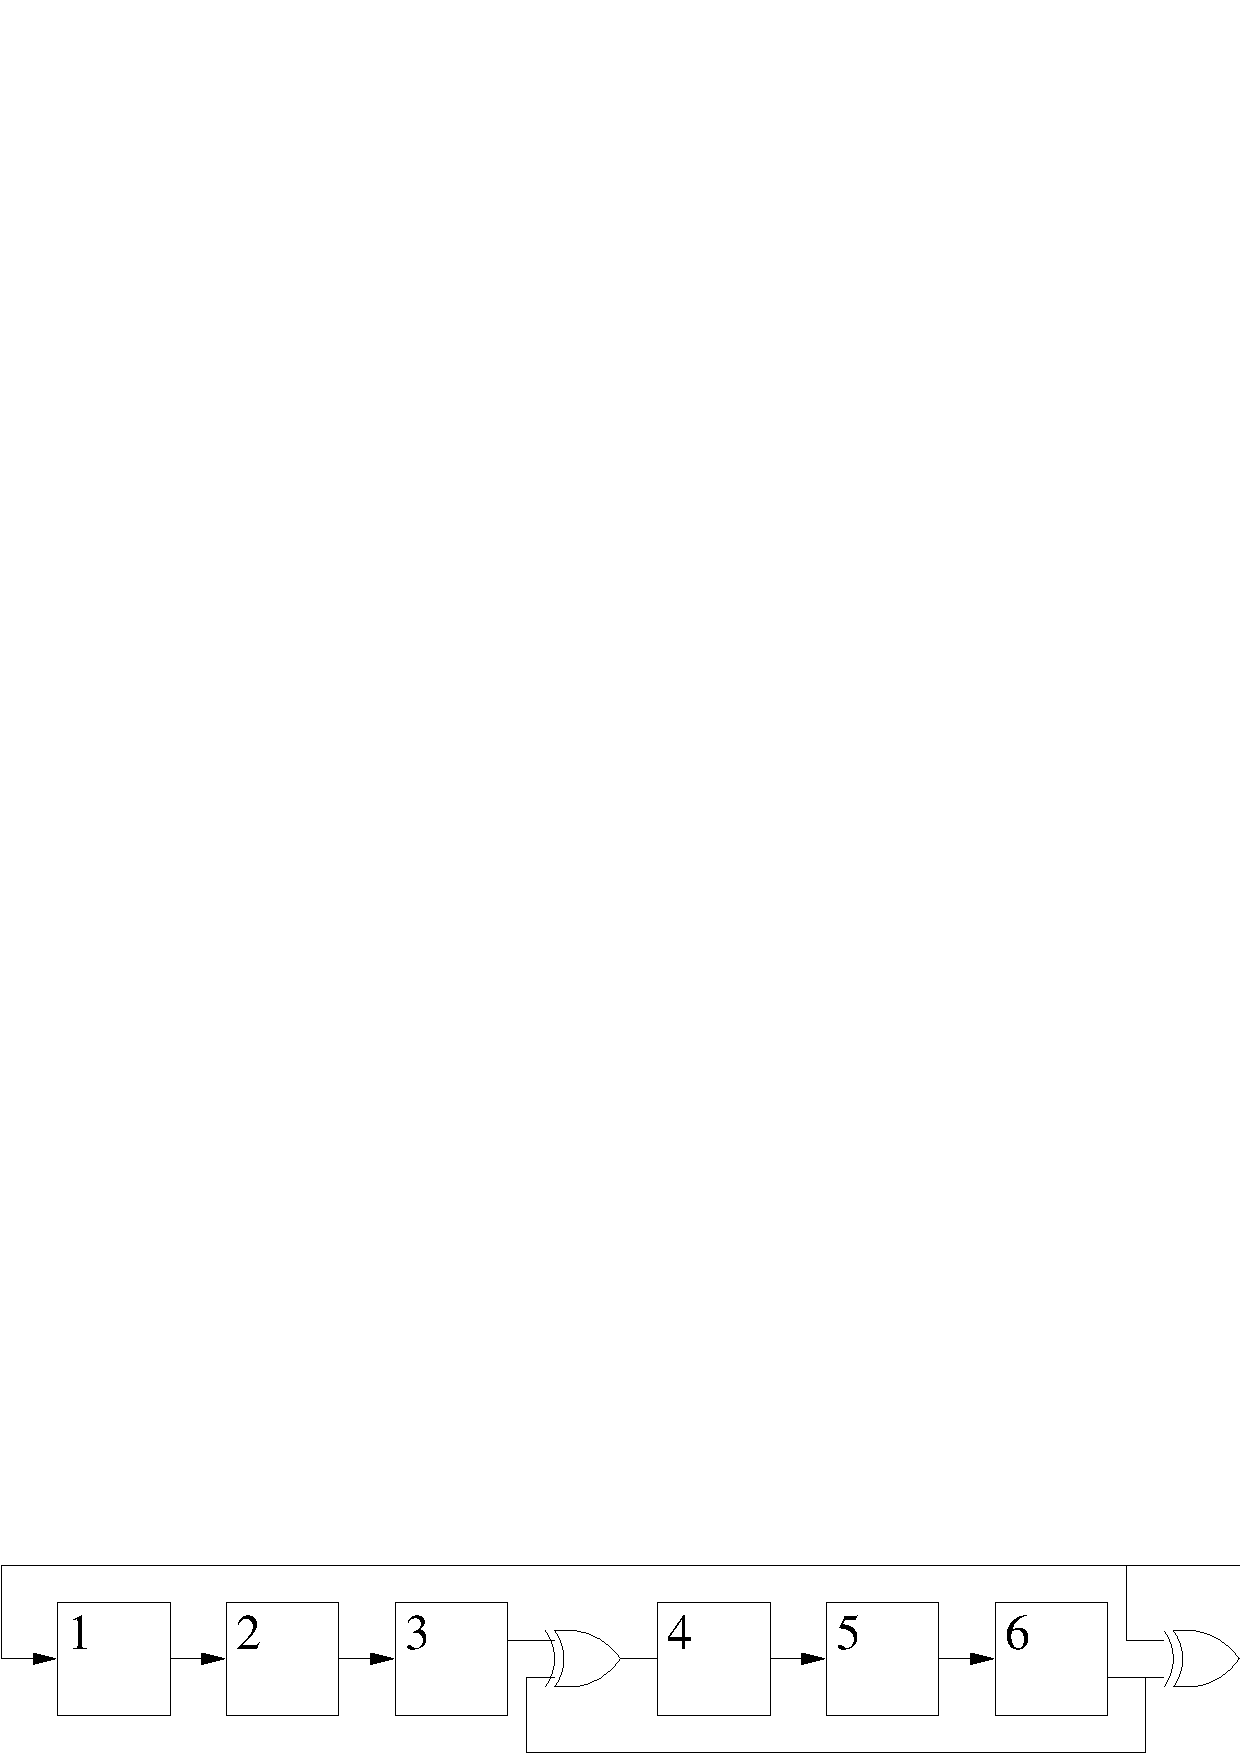
\includegraphics[width=\linewidth]{images/mfsr8.pdf}
\caption[An 8-bit MFSR with a cycle size of 255]{An 8-bit MFSR (Multiple
Feedback Shift Register) with a cycle size of 255. The total logic required is
only eight D-type flip-flops and two XOR logic gates. \textit{Image courtesy
of R. Ward}~\cite{MFSR_List}}
\label{CPU_MFSR8}
\end{center}
\end{figure}


\section{Processor Performance}
To improve the performance of a processor, the biggest gains are made by making
the common operations fast~\cite{Comp_Arch}. The primary computational task of
OpenVGA's processor is to convert data sent to OpenVGA into the framebuffer's
data format. This consists of mainly arithmetic, bit-wise logic, and memory
operations. Arithmetic and logical operations take just one clock cycle. Memory
operations are far slower but a fast data-cache has been developed (see
Section~\ref{MEM_Cache}), reducing the average delay to only about five processor
clock cycles.


% \subsection{Amdahl's Law}
Amdahl's law defines the speedup obtained from a given enhancement made to a
machine~\cite{Comp_Arch}. This speedup is based on the performance for the entire
task, with and without the enhancement, $\tau_E$ and $\tau_O$ respectively. For a
given enhancement to a CPU, the speedup is the ratio defined as

\[
\mathrm{Speedup} = \frac{\tau_O}{\tau_E}
\]

Amdahl's Law allows the effect of enhancements to the CPU to be objectively
evaluated. For example, consider the question: ``How much of a performance effect
does doubling the number of processor data-transports and FUs give?''

\begin{flushleft}\textbf{Answer:} A memory operation for the text-mode conversion
algorithm typically takes about 5 clock cycles, due to the benefit of
data-caching. If about one third of the instructions contain memory operations
(see Section~\ref{CACHE_Justification}), and all other operations complete in one
clock cycle, and about two million memory accesses are required to redraw one
frame, then the time in cycles to redraw one frame is

\begin{eqnarray*}
\tau_O	& = & 5 \times 2\times10^6 + 4\times10^6 \\
		& = & 14\times10^6
\end{eqnarray*}

If the number of transports and functional units are doubled, giving a perfect
speedup of two for non-memory instructions, then the total speedup would be

\begin{eqnarray*}
\mathrm{Speedup}	& = & \frac{\tau_O}{\tau_E}	\\
					& = & \frac{14\times10^6}{12\times10^6}	\\
					& \approx & 1.17	\\
\end{eqnarray*}
\end{flushleft}

The resulting CPU would nearly be twice as large though. The actual speed-up
factor will be less than two because of scheduling difficulties. And the Xilinx
PAR tool would find the design harder to route, likely reducing processor
operating frequency too. So doubling the number of transports would not be an
efficient modification in this case since the FPGA logic resources are limited
and the speedup minimal.


\section{Tools \& Testing}
One of the processors designed and implemented within OpenVGA, TTA16, has an
unsual architecture, and it would be a non-trivial task to adapt an existing open
source assembler, and especially a compiler, to this architecture. It would have
been extremely tedious to generate large quantities of object code too. Therefore
an assembler was needed for both TTA16 and RISC16.

Testing the two processors was initially done with the Icarus Verilog simulator,
and later with hardware testbenches. Simple TTA16 and RISC16 programs were
written for processor testing to verify correct operation of the FUs. The CPU of
the host PC can access all of OpenVGA's memory using a Linux kernel module.

\subsection{Object Code Generation}
Processors execute instructions in the form of object code, which is a binary
representation of an instruction. Typically, assemblers, interpreters, and
compilers are used to generate object code. There are currently no interpreters
or compilers that have TTA16 or RISC16 as an output target since these processors
have custom instruction sets. There is an assembler for each of these processors
though.

\subsubsection{TTA16 Assembler}
\filedescript{Roy Ward, Patrick Suggate}{assemble}{A general-purpose TTA
assembler which loads an XML processor description from a
file prior to assembly.}{/data/tta16.xml}{/src/fw\_tta16/*.S}{GPL}

An assembler was created by R. Ward~\cite{XML_Assembler} for another project, and
additional features were added by him to assist this project. This assembler
reads in a processor definition file, which is stored as an XML file, and then
assembles the assembly language source file in accordance to the definition in
the XML file. This assembler was designed for TTA applications and it supports
explicit Instruction Level Parallelism\glossary{name={ILP},
description={Instruction Level Parallelism}} (ILP) (see the TTA16 programming
guide in Appendix~\ref{TTAPROG_TTA16_memcpy} for an example of this).

Below is an excerpt from \texttt{tta16.xml}, the file defining the TTA16
instruction set. This fragment encodes the available destination registers for
transport-0 of TTA16\footnote{This bit-field is called $DST0$ in the instruction
format diagram, see Figure~\ref{TTA_Instruction_Format}} , and has been included
to demonstrate the syntax. The XML encoding is very general purpose, and has been
used for other TTA processors as well~\cite{TTA_Ray_Trace}.

\begin{center}
\begin{minipage}{0.8\linewidth}
\footnotesize
\verbatiminput{source/tta16_excerpt.tex}
\normalsize
\end{minipage}
\end{center}

\noindent The first line in a TTA16 assembly source file is typically:
\begin{center}
\begin{minipage}{0.5\linewidth}
\begin{verbatim}
architecture:tta16
\end{verbatim}
\end{minipage}
\end{center}

This line specifies the name of XML file to use when assembling this file and
this line has to precede any assembly language. Comments may precede this line,
and since the \texttt{m4} macro processor was used as a preprocessor with this
assembler, to allow the use of constants and macros for common tasks, macro
definitions will often be at the start of TTA16 assembly files too.

A TTA16 instruction encodes the move operations for each of its four transports.
Each of these four \texttt{move} fields are separated by commas, and an empty
field indicates no-operation for that transport within the current instruction.

Arrows (a minus and a greater-than, \texttt{->}) are a required part of the
assembly syntax and they graphically indicate the direction of data flow. Curly
braces surround all instructions, and instructions can be preceded by an optional
label, before the braces. More information on TTA16 assembly and programming is
in Appendix~\ref{TTA_Programming}, but here is an example of the TTA16 assembly
syntax:
% \footnotesize
\begin{center}
\begin{tabular}{l l l l l l l l l}
\tt loop: & \tt \{r1 & \tt ->rad, & \tt 2 & \tt ->sub, & & & \tt ,r2 \tt
\}
\end{tabular}
\end{center}
Shown above is a label, \texttt{loop:}, two general-purpose registers
(\texttt{r1} and \texttt{r2}), and two special-purpose registers
(\texttt{rad} and \texttt{sub}). The third \texttt{move} field is empty,
indicating no-operation, and the fourth transport has only one argument,
\texttt{r2}. This is the source for the data-move, the destination is always the
common ALU operand register \texttt{com}, and is therefore excluded from the
syntax.


\subsubsection{RISC16 Assembler}

\filedescript{Patrick Suggate}{r16asm.py}{A simple RISC16
assembler.}{/src/r16asm.py, /src/CodeCleaner.py, /src/AsmParse.py,
/src/Emit.py}{/src/fw\_risc16/*.S}{GPL}

RISC16 uses a custom assembler, written in Python specifically for this
processor. Example code written for this assembler is shown in
Appendix~\ref{RISCPROG_Memcpy}. RISC architectures are not explicit-ILP
processors, and the syntax used with the TTA assembler is somewhat cumbersome for
RISC16. Additionally, RISC16 had some instructions that were hard to define
within the XML processor definition file (especially the immediate constant field
of the \texttt{i12} instruction prefix). This justified the creation of yet
another assembler.

\noindent The general form of a valid line of assembly code that is accepted by
this assembler is:

\begin{center}
\tt		[label:] mnemonic [arguments]
\end{center}

The \texttt{label:} field is used to label the destination of branches, and to
label constants so they can be referenced within the code. The \texttt{mnemonic}
field is a keyword identifying the desired instruction, which is translated into
an opcode (condensed form of operation-code\glossary{name={opcode},
description={Condensed form of operation-code}}) in the final phase of the
assembler. Fields surrounded by square braces indicate that the field can be
optional. All constants are required to have a label, and most instruction
require arguments.

An overview of the algorithm the assembler uses to generate an output file is:

\begin{enumerate}
  \item Parse command-line options for the input file name, the optional output
  file name, and the assembler options.
  \item Read in assembly file, line-by-line. Line numbers are
  stored, with each line, at this point. This is needed so useful error
  messages can be generated later.
  \item Remove comments and extra white-spaces, throwing away lines containing
  no code or no assembler directives.
  \item Tokenise each of the remaining lines according to the simple format
  discussed above.
  \item The parser takes the stream of tokens, builds a table of constants, and
  then a table of branch destination labels. The next parse step is
  evaluating the instruction arguments, which involves substituting any
  labels, in the arguments, for its corresponding constant or address value.
  The final parse step is to evaluate any argument that represents a numerical
  value, the set arithmetic and bit-wise logical operations used in the C
  language is accepted.
  \item Since both TTA16 and RISC16 use an MFSR instead of a standard PC
  incrementer, the generated object code needs to be reordered according to
  the MFSR count order. Since the count order is pseudo-random, it will span
  the entire instruction RAM block(s), so before reordering the instruction
  stream, it is padded with \texttt{nop} (no-operation) instructions so that it
  contains the same number of instructions as the block RAMs can hold.
  \item The parsed and reordered instruction mnemonics and arguments are
  matched against valid instruction formats, and upon match, the hexadecimal
  representations of the object code is then emitted to the output file.
\end{enumerate}


\subsection{Processor Testing and Testbenches}
Initially, each FU was developed and tested using the FOSS (Free and Open-Source
Software) simulator Icarus Verilog\footnote{Icarus Verilog is available on the
Internet from http://www.icarus.com/eda/verilog/}. Processors can be very
difficult to debug, especially RISC16 with its many hazard detection flags and
states, so it was important that the components were well tested first. Another
FOSS Electronic Design Automation\glossary{name={EDA}, description={Electronic
Design Automation}} (EDA) application, GtkWave\footnote{GtkWave is available on
the Internet from http://gtkwave.sourceforge.net/} was used to display the timing
diagrams of the simulated signals, which were saved to a VCD\glossary{name={VCD},
description={Value Change Dump}} output file by Icarus.

When a processor had been developed to the point where it simulated as expected,
larger quantities of test code were written, with a disassembler coded within
the processors HDL source displaying the instructions (with input and output
values) being executed. The MMIO functionality and correct data cache operation
could then be verified.

Once a design was believed to operate correctly, hardware testbenches were
synthesised and uploaded to OpenVGA, at first just running code for a trivial
task like flashing some LEDs. Figure~\ref{TTA16_Synthesis} shows the synthesiser
output for one of the TTA16 hardware testbenches. As can be seen, TTA16 is very
fast for a processor implemented on Spartan-3\footnote{It is often estimated that
an FPGA has about one-tenth the performance of an ASIC made with the same
manufacturing process, in this case 90 nm.}.

The Verilog synthesiser used was ISE WebPack$^{TM}$ 9.1 developed by Xilinx,
since it is free of charge, though proprietary, and available for both the Windows and
GNU/Linux operating systems. Being free, it keeps with the goal of OpenVGA being
a low-cost platform for development.


\begin{figure}[h!]
\begin{center}
\Ovalbox{%
	\begin{minipage}{0.9\linewidth}
		\begin{center}
		\begin{minipage}{0.8\linewidth}
\begin{verbatim}

Timing summary:
---------------

Timing errors: 0  Score: 0

Constraints cover 2115 paths, 0 nets, and 1452 connections

Design statistics:
   Minimum period:   5.249ns (Maximum frequency: 190.512MHz)
   Minimum input required time before clock:   6.874ns
   Maximum output delay after clock:   9.816ns


Analysis completed Wed Dec 24 08:08:07 2008
-------------------------------------------
\end{verbatim}
		\end{minipage}
		\end{center}
	\end{minipage}}
\caption[TTA16 synthesis timing report]{Xilinx Place and Route (PAR) report
showing the synthesised TTA16 hardware testbench timing and routing information.}
\label{TTA16_Synthesis}
\end{center}
\end{figure}





%%%%%%%%%%%%%%%%%%%%%%%%%%%%%%%%%%%%%%%%%%%%%%%%%%%%%%%%%%%%%%%%%%%%%%%%%%%%%
%%%%%%%%%%%%%%%%%%%%%%%%%%%%%%%%%%%%%%%%%%%%%%%%%%%%%%%%%%%%%%%%%%%%%%%%%%%%%
\section{TTA16}
\label{TTA16}

\mmodule{Patrick Suggate}{tta16}
{A 16-bit, TTA processor logic core designed for use with FPGAs.}
{/rtl/cpu/tta16/tta16.v, /rtl/cpu/tta16/tta16.xml,
/rtl/cpu/tta16/tta\_stream4to4.v, /rtl/cpu/tta16/tta\_stream4to8.v,
/rtl/cpu/tta16/tta\_stream8to8.v, /rtl/cpu/fastbits.v}
{/sim/cpu/tta16\_tb.v}{GPL}

TTA16, is a small, fast, 16-bit, transport-triggered, processor logic core
designed for OpenVGA initialisation, state management, and the data processing
tasks for emulating VGA functionality. TTA16 features a three-stage pipeline,
four data transports, explicit ILP, 16 general purpose registers, up to 32-bit
memory address support, logic and arithmetic operations, a multiplier, a fast
local instruction store, and a fast Wishbone bus interface to access OpenVGA
Wishbone bus peripherals, including the system memory.

TTA16 is a partially-connected TTA, each FU can only get data from, and place
data on, a subset of the processor transports. The FU and data-transport
connectivity of TTA16 is shown in Figure~\ref{TTA16_Tranport_View}. Partially
connected TTAs allow the use of smaller multiplexers for connecting FUs to
transports, resulting in smaller and faster designs~\cite{arnold1997dtr}.

\begin{figure}[h!]
\begin{center}
\includegraphics[width=\linewidth]{diagrams/tta16_henk.pdf}
\caption[TTA16 transports and functional units overview]{TTA16 transport-based
diagram which shows the connections between transports and FUs.}
\end{center}
\label{TTA16_Tranport_View}
\end{figure}

Even though TTA16 is a very capable processor, when synthesised for the Spartan-3
architecture TTA16 uses only approximately 220 logic slices\footnote{This is when
XST is set to optimise for speed, when optimising for size it uses even less.}
which is very small for the feature set. Additionally, the maximum clock rate at
which it will run is up to 190 MHz (see Figure~\ref{TTA16_Synthesis}), very fast
for a processor implemented within the Spartan-3 FPGA family. A comparison with
other Spartan-3 based processors is shown in Table~\ref{SUMMARY_CPU_Table}.


\subsection{Introduction to TTA Processors}
A TTA processor is different from more common processors, like RISC and CISC
based processors such as ARM, SPARC, x86, Power, and MIPS. TTA instructions are
simply a list of data moves for each transport that the processor has to perform.
For comparison, instructions of more traditional architectures typically specify
the desired operation and the data to use for that operation.

To perform useful work, processors need FUs (Functional Units) that carry out
some operation, like branching, memory load and store, and subtraction and other
calculations. Work is performed within a TTA processor by transporting values to
special purpose registers, some of which can trigger side-effects, like
computations. There are three main classes of registers

\begin{itemize}
  \item Trigger Registers: These trigger the start of operations within FUs.
  The operations which are initiated depend on the FU, they can be an
  operation like a memory write, or a subtract, or whatever computations the FU
  supports.
  \item Operand Registers: These supply additional values for an operation, a
  subtract requires both a subtrahend and a minuend, for example. Unlike
  trigger registers, writing to an operand register has no side-effects. The
  number of operand registers required by a FU varies, and can even be zero.
  \item Result Registers: These are the results of computations by FUs, they
  can have a latency of zero or more cycles, and FUs can have more than one
  result register, like the multiplier (see Section~\ref{TTA_Multiply}) for
  example.
\end{itemize}

Figure~\ref{TTA_Simple_Add} demonstrates how to perform a calculation in a TTA
processor, in this case an addition. RISC-type assembly code is given for
comparison. The simple addition example looks to be a clear win to the RISC
processor, even if it is assumed that a TTA can be made to operate at a 50\%
higher clock rate (see Table~\ref{SUMMARY_CPU_Table}).

Also note that the RISC instruction reads two values from the Register
File\glossary{name={RF}, description={Register File}} (RF, \texttt{r0} and
\texttt{r1}), and writes back one (\texttt{r0}) This requires the RF to have a
bandwidth of three operations per clock cycle, or else it will take longer than a
single cycle to complete, or maybe affect/restrict other instructions.

\begin{table}[h!]
\begin{center}
\Ovalbox{
	\begin{tabular}{l l}
	\begin{minipage}{0.4\linewidth}
    	\begin{center}
		\begin{tabular}{l l}
        	\multicolumn{2}{c}{RISC-type instructions}	\\
        	\\
	    	\texttt{add} & \texttt{r0, r0, r1}	\\
	    		&				\\
	    		&				\\
	    \end{tabular}
        \end{center}
	\end{minipage} &
	\begin{minipage}{0.4\linewidth}
    	\begin{center}
		\begin{tabular}{l l l l}
        	\multicolumn{4}{c}{TTA-type instructions}	\\
        	\\
			\tt	\{\tt r0 & \tt -> & \tt add & \} \\
			\tt	\{\tt r1 & \tt -> & \tt add$_t$ & \}\\
			\tt	\{\tt sum & \tt -> & \tt r0 & \} \\
    	\end{tabular}
        \end{center}
	\end{minipage}	\\
\\
	\end{tabular}
}
\caption[A simple addition operation to demonstrate the TTA concept]{A simple
addition operation to demonstrate the TTA concept. The addition is only
initiated once a write is made to the addition-trigger register (add$_t$).}
\label{TTA_Simple_Add}
\end{center}
\end{table}


For the second example, lets say the task is to sum four numbers, stored in
\texttt{r0-3}, and the example TTA now has an ILP of two\footnote{An ILP of
four~\cite{corporaal1993maa} is common but much higher than this was experimented
with by Henk Corporaal\cite{corporaal1993maa}}. As Figure~\ref{TTA_Accumulate}
shows, the new TTA code now fares a little better, it can even be considered to
win if it can operate at a 50\% percent higher clock rate. The TTA still requires
less register-file bandwidth as well, five accesses compared to nine of the RISC.

\begin{table}[h!]
\begin{center}
\Ovalbox{
	\begin{tabular}{l l}
	\begin{minipage}{0.4\linewidth}
    	\begin{center}
		\begin{tabular}{l l}
        	\multicolumn{2}{c}{RISC-type instructions}	\\
        	\\
	    	\texttt{add} & \texttt{r0, r0, r1}	\\
	    	\texttt{add} & \texttt{r0, r0, r2}	\\
	    	\texttt{add} & \texttt{r0, r0, r3}	\\
	    		&				\\
	    \end{tabular}
    	\end{center}
	\end{minipage} &
	\begin{minipage}{0.5\linewidth}
	\begin{tabular}{l l l l l l l}
        	\multicolumn{7}{c}{TTA-type instructions}	\\
        	\\
	\tt	\{\tt r0 & \tt -> & \tt add, & \tt r1 & \tt -> & \tt add$_t$ & \} \\
	\tt	\{\tt r2 & \tt -> & \tt add, & \tt sum & \tt -> & \tt add$_t$ & \}\\
	\tt	\{\tt r3 & \tt -> & \tt add, & \tt sum & \tt -> & \tt add$_t$ &	\}\\
	\tt	\{		 &		  &			 & \tt sum & \tt -> & \tt r0 & \} \\
    \end{tabular}
	\end{minipage}	\\
\\
	\end{tabular}
}
\end{center}
\caption[TTA Accumulate Example]{TTA Accumulate Example. Accumulate four
numbers and store the result in \texttt{r0}. This TTA has an ILP of
two, meaning two data moves are performed every clock cycle.}
\label{TTA_Accumulate}
\end{table}

Due to TTA16's explicit ILP, four data moves occur per instruction. TTA16 is not
fully connected though, each execution stream cannot access all of the processors
registers, just a smaller subset. This approach makes the transports simpler, and
therefore faster, and if the connections are chosen well, the net effect is a
performance increase~\cite{arnold1997dtr} due to allowing a higher clock rate.

Even with four moves per clock, TTA16 still required less RF bandwidth than
RISC16 (a general feature of TTAs~\cite{hoogerbrugge1994rfp}), so the RF is only
half the size of RISC16 (see Section~\ref{RISC16_RF}), 16 Spartan-3 slices (32
LUTs) versus 32 of RISC16. Within OpenVGA, the total RF bandwidth of TTA16 is
identical to RISC16 since a two port RF operating at 150~MHz has the same
bandwidth as three ports at the 100~MHz of RISC16\footnote{The operating
frequencies of TTA16 and RISC16 are lower than their absolute maximum values due
to routing factors, the data cache frequency, and the Wishbone bus clocks.}.


\subsection{Internal Tri-States vs. Multiplexers}
Multiple FUs are connected to the four transports of TTA16, but since only one FU
result register can place its value onto a transport during any given clock
cycle, there needs to be hardware that selects the register to be placed on the
transport. Typically, multiplexers and internal tri-states are used, but the
Spartan-3 family does not include internal tri-states, unlike previous FPGA
families from Xilinx~\cite{Xilinx_SP3_DS}\footnote{Internal tri-states were
implemented within the Virtex II Family via primitives called TBUFs. This was
often of limited value since the number was relatively scarce and the locations
fixed. The Spartan-3 does not have any TBUFs.}.

The Spartan-3 does support internal pull-up networks though~\cite{Xilinx_SP3_DS}.
Internal pull-ups are implemented using the general-purpose, four-input LUTs, but
using them as internal pull-ups often requires adding one extra layer of LUTs.
This extra layer of LUTs, and the routing cost, lead to a large performance
penalty as shown in Table~\ref{TTA_Routing_Network}. Multiplexers are a clear win
in this situation, so they were used for TTA16.

\begin{table}[h!]
\begin{center}
\begin{tabular}{l c c}
Routing Method	& Speed & Size \\
				& (MHz) & (Slices) \\
\hline
Internal Pull-ups & 147 & 245 \\
Multiplexers & 190 & 203 \\
\end{tabular}
%\normalsize{}
\caption[Synthesis results comparing multiplexers and internal
pull-ups]{Synthesis results comparing multiplexers and internal pull-ups.}
\label{TTA_Routing_Network}
\end{center}
\end{table}



\subsection{The TTA16 Pipeline}
TTA16 is pipelined so that the work of executing a single instruction is spread
over multiple clock cycles. Instructions are first fetched, data are then moved
via transports, and then the specified functional units are triggered.

\begin{figure}[h!]
\begin{center}
\includegraphics[width=8cm]{diagrams/tta16_pipeline.pdf}
\caption[TTA16 pipeline overview]{TTA16 pipeline overview showing a three-stage
pipeline.}
\end{center}
\label{TTA16_Pipeline}
\end{figure}

A new instruction is fetched every clock cycle, except during a memory read/write
interlock. There are up to three instructions ``in-flight'' within the pipeline
(see Figure~\ref{TTA16_Pipeline}. The purpose of pipelining is to allow more
instructions to be issued per unit time, but each instruction will probably take
longer to execute than a the same instruction in non-pipelined, but otherwise
similar, processor\footnote{This is due to two main reasons, the first being that
the pipeline registers each add a small combinatorial component. The second
reason being that the total work required to execute one instruction will not be
uniformly divided amongst each pipeline stage, a critical path will limit the
maximum frequency, other paths will be slightly quicker.}. It is a form of ILP
since there are three instructions being processed simultaneously within the
TTA16 pipeline, though each in a different stage.


\subsection{Functional Units}
\label{TTA16_FUs}
The basic design of a TTA processor is several transports connecting multiple
FUs together. This is essentially true for all processors but the concept of
using transports to move data between FUs is very explicit with TTA processors.


\subsubsection{Program Counter and Flow Control}

\regdescript{Program Counter}{bra, jb, jnb, jz, jnz}{N/A}{pc}

There is only one trigger register but the aliases determine the condition
that is required to be met in order to follow the branch. Branches not followed
are treated as NOPs.

All branch destinations are determined by absolute addresses, there is no
support for relative branches. This is due to the Program Counter (PC) using an
MFSR as its increment operator~\cite{MFSR_List}. MFSR propagation delays are
lower since there is no carry logic and the logic depth is one.

The PC is only 10-bits wide, and the immediate field of a TTA16 instruction is
up to 11-bits wide, so loading the PC with the value from the immediate
field of the instruction allows all locations in instruction memory to be
reached. Registers can also be used as sources for branch instructions, since
the PC is treated as just another FU register, any value can be written to it.

\begin{figure}[h]
\begin{center}
\includegraphics[width=9cm]{diagrams/pc_unit.pdf}
\caption[The PC increment and branch unit]{The PC increment and branch unit. \\
The incrementer (labelled ``+1'') is actually implemented as an MFSR to
reduce PC calculation latency~\cite{MFSR_List}.}
\label{CPU_PC_Unit}
\end{center}
\end{figure}

There is an instruction fetch delay (due to pipelining) of one clock cycle.
This delay causes an extra cycle of latency between the branch instruction being
executed and the instruction at the branch address fetched and ready to
execute. The gap of one cycle, between the branch being executed and the
instruction fetched from the branch destination, there are a couple of options
as to what the CPU can do:
\begin{itemize}
  \item It can either stall (or issue a NOP).
  \item It can execute the instruction following the branch anyway, since it has
already been fetched.
\end{itemize}

The instruction(s) immediately following a branch, which are executed, are called
branch delay slot instructions. Processors that support the execution of
instructions in branch delay slots include SPARC~\cite{SPARC_Arch},
MIPS~\cite{britton2004mal}, PA-RISC, ETRAX CRIS, and SuperH~\cite{SuperH}. This
is also the approach that TTA16 uses. This means that the instruction following a
conditional branch is always executed, irregardless of whether the branch is
taken or not. It is often possible to fill this slot with a useful instruction
(see Figure~\ref{TTAPROG_TTA16_memcpy}, but if it is not possible to do something
useful, this slot must be filled with a NOP.


\subsubsection{Register File}

\regdescript{Register File}{r0-r15}{N/A}{r0-r15}
% Register Descriptions:
% 
% \begin{flushleft}
% \begin{tabular}{l l}
% \textbf{Trigger Register(s) and Aliases:} & R0-15 \\
% \textbf{Operand Registes(s) and Aliases:} & none \\
% \textbf{Result Register(s)}: & R0-15 \\
% \end{tabular}
% \end{flushleft}

These are 16, 16-bit, general-purpose registers, and function in the same way as
general-purpose registers in RISC architectures. Up to two of these register can
be read per clock cycle, and up to one write. All transports can read from the
RF, but only transport three can write results back to the RF. (See
Appendix~\ref{TTA_Programming} to obtain more details on the quirks and
restrictions on RF use.)

The TTA16 Register File (RF) was implemented using Spartan-3 distributed RAM
resources. There is hardware support for using this distributed RAM in
dual-port mode allowing a read and a write to occur within each processor clock
cycle (though reads are actually asynchronous with this primitive, but they
were pipelined anyway to increase performance).


\subsubsection{Bitwise Operations}
\label{TTA_Bitwise}

\regdescript{Bitwise Unit}{and, nand, or, xor, cmp}{com}{bits, zf}

The bitwise FU can perform one of four logic operations on the 16-bit input
values, and these are selected by the two-bit mode input, which is set
depending on the alias used. These modes are shown below:

\begin{center}
\begin{tabular}{l c}
\multicolumn{1}{l}{Logical} & Mode \\
Operation & Bits \\
\hline
AND		& 00 \\
NAND	& 01 \\
OR		& 10 \\
XOR		& 11 \\
\end{tabular}
\end{center}

The CMP (CoMPare) alias performs an XOR within this FU, but also simultaneously
triggers a subtract operation. The intended side-effect is that both the CPU
flags, the ZF and BF, are set at once, which can be useful for conditional
branches.

The bitwise FU also asserts/deasserts the ZF, depending on whether the result
of a bitwise operation contains all zeroes, or not. To calculate the value of
the ZF, the carry-chain is used (see Figure~\ref{CPU_Bitwise_Unit}), saving an
additional cycle by not needing a separate zero test unit.

The actual output of the bitwise FU is the inverse of the desired result, due to
the carry-chain's MUX requiring a ``1'' input to propagate the carry signal. But
there is no performance penalty when inverting the bitwise result to get the
desired value though, since the TTA transport multiplexers perform this without
penalty. This is because these multiplexers are implemented using the same
arbitrary function LUT4s (four-input Look-Up Tables) as used in this FU.

\begin{figure}[h!]
\begin{center}
\includegraphics[width=8cm]{diagrams/bitwise_unit.pdf}
\caption[3-Bit, Bitwise Operations Unit]{3-Bit, Bitwise Operations Unit. \\
This shows how a 3-bit, bitwise operations FU implementation would look when
synthesised for the Spartan-3 architecture. The inputs are a[2:0], b[2:0],
and the mode m[1:0]. The bitwise operations FU takes advantage of the fast
carry chain logic to compute the value of the ZF (Zero Flag) simultaneously
with the bitwise result, and so implementing the ZF uses only one additional
DFF (See the accompanying text for a full description).}
\label{CPU_Bitwise_Unit}
\end{center}
\end{figure}

The latency once synthesised is about 4.5 ns, depending on the optimisations used
and how complex the overall design is. The total logic cost, including the zero
flag is only 17 LEs, less than nine slices. The Verilog source for this FU uses a
Xilinx specific primitive, MUXCY, which means that this FU will only synthesise
when targeting a subset of Xilinx FPGA architectures. The MUXCY primitive had to
be explicitly instantiated since the Xilinx optimiser failed to pack the design
using this primitive automatically.

The carry chain within the Spartan-3 FPGA runs vertically so all elements of the
bitwise FU are placed vertically adjacent, but the Xilinx Synthesis
Tool\glossary{name={XST}, description={Xilinx Synthesis Tool}} (XST) handles this
automatically, explicit use of the MUXCY primitive ensures this.

\subsubsection{Subtractor}

\regdescript{Subtractor}{sub, sbb, cmp}{com}{diff, bf}
% Register Descriptions:
% 
% \begin{flushleft}
% \begin{tabular}{l l}
% \textbf{Trigger Register(s) and Aliases:} & SUB, SBB, CMP \\
% \textbf{Operand Registes(s) and Aliases:} & COM \\
% \textbf{Result Register(s)}: & DIFF, BF \\
% \end{tabular}
% \end{flushleft}

The Spartan-3 has fast carry chain logic which is designed to increase the
speed of arithmetic operations (typically additions, subtractions, and
multiplications) that are implemented using general-purpose logic resources.
This carry chain also supports the borrow functionality needed for subtraction.
Consequently, subtract operations take about 5 ns for a 16-bit addition in a
synthesised design, but only an extra 0.064 ns for each extra bit width of the
input numbers, as long as PAR does a good job (see
Figure~\ref{CPU_Bitwise_Unit} for an example of the fast carry/borrow chain).

The borrow chain implementation uses the MUXCY primitive (like with the
bitwise FU shown in Section~\ref{TTA_Bitwise}) but also uses an
XORCY\footnote{The CY suffix of XORCY denoting that its intended use is to be
part of the carry chain, like with the MUXCY primitive, but they can be freely
instantiated for any purpose the designer can think of. They have a more
restrictive connection scheme than LUT4s though, so often they are only useful
as carry/borrow logic.} primitive and a different connection scheme.
Fortunately the XST places these automatically for additions and subtractions,
since this is a common use-case, so implementation of subtractors only takes as
many LEs as there are bits in the widest input number.

The subtractor FU also supports the subtract-with-borrow operation which
allows subtract operations with numbers longer than 16-bits to be implemented
quite efficiently. This is achieved by having a processor Borrow Flag (BF)
which is set by any subtract operation, but only used for SBB and conditional
branch operations. This BF requires an additional LE which brings the total for
TTA16's subtract FU to 17 LEs.

As explained above, the CMP alias simultaneously triggers an XOR in the bitwise
FU and a SUB within this FU.


\subsubsection{Multiplier}
\label{TTA_Multiply}

\regdescript{Multiplier}{mul}{com}{plo, phi}

Within every Spartan-3 FPGA there are embedded multipliers capable of operating
at about 200 MHz~\cite{Xilinx_SP3_DS}. These embedded multipliers take two 18-bit
(or less), signed integers and calculate a 36-bit, signed product. Both the upper
(PHI) and lower (PLO) halves of the 36-bit product can be selected, so supporting
multiplications on numbers wider than 18-bits is fairly easy and
efficient\footnote{It is still quite complicated since the processor does not
have an adder for adding partial products. Negations and the subtractor has to be
used.}.

Within each embedded multiplier there exists a pipeline register, use of which
is optional, so a registered multiplier can be implemented using no additional
general-purpose logic elements.

Due to the way Xilinx chose to implement these multipliers, there exists a
combinatorial delay component on either side of the pipeline register. When
synthesising TTA16, this combinatorial component causes the path from the
multiplier output to transport register to be the critical path. This is the
path which limits TTA16 performance to about 190 MHz.

There exists a synthesis flag for TTA16 to optionally use an extra pipeline
stage to hide this combinatorial component, but this also increases the size
of TTA16 which, due to the extra routing costs, does not actually increase
clock rate either, and adds an extra cycle of latency penalty on multiply
operations too, so this option was left disabled.


\subsubsection{Wishbone Bus Interface}

\regdescript{Load-Store Unit}{rad, wad}{mem, rseg, wseg}{mem}

To support large addresses, with a native CPU data size of 16-bits, a memory
segment model is used. Each segment consists of $2^{16}$ (65536), 16-bit words,
or 131072 bytes. There can be up to $2^{16}$ of these segments to give a total
addressable memory limit of 8 GB.

The registers \texttt{rseg} and \texttt{wseg} are (respectively) the segments for
memory read and write accesses, and these are set via writes to the special
function registers FU. These segment values are concatenated with the lower
16-bit addresses, \texttt{rad} and \texttt{wad}, for reads and writes
respectively, to produce the full 32-bit, word-aligned address.

The contents of the \texttt{mem} register are written to the Wishbone bus when
WAD is triggered, and the contents of \texttt{mem} are set after the Wishbone bus
read transaction, triggered by a write to \texttt{rad}, completes. Both the
registers called \texttt{mem} are actually different registers too, so a
\texttt{mem} to \texttt{mem} transport is needed when performing a memory copy.

Memory access, for example, has an undeterminable latency, it depends on Wishbone
bus activity and whether the SDRAM is refreshing. When a Wishbone access it
triggered, TTA16 asserts the interlock signal to stall the CPU until the Wishbone
bus operation completes. Due to this stalling, Wishbone access is the slowest CPU
operation, but interlocking ensures correctness.


\subsubsection{Special Function Registers}

% Register Descriptions:

\regdescript{System Registers}{msr}{com}{N/A}

There are currently five special registers implemented, two are the segment
registers, \texttt{wseg} and \texttt{rseg}, as detailed above. The other three are used for
modifying the contents of the instruction memory.

\begin{center}
\begin{tabular}{c l}
MSR		& Register	\\
Index	& Name	\\
\hline
0	& RSEG	\\
1	& WSEG	\\
2	& IADR	\\
4	& IDAT$_{LO}$	\\
5	& IDAT$_{HI}$	\\
\end{tabular}
\end{center}

IADR is the 10-bit address of the instruction to overwrite, and since
instructions are 32-bits wide, it takes two 16-bit writes, the LSW of the
instruction is written to IDAT$_{LO}$, while the MSW is written to IDAT$_{HI}$.

The primary purpose is to allow new pages of instructions to be fetched from main
memory, though it would be possible to use this mechanism for self-modifying
code, like setting the value of a constant before entering in a tight-loop.


\subsection{Instruction Format}
TTA16 has just one instruction format (see Figure~\ref{TTA_Instruction_Format}),
a list of data moves between registers and a some immediate data fields. The
immediate is used for specifying constants used in a program, like a count
value or an address offset, or for specifying a register index when performing
a RF read or write.

\begin{figure}[h!]
\begin{center}
\includegraphics[width=\linewidth]{diagrams/tta16_instr.pdf}
\caption[TTA16 instruction format]{TTA16 instruction format. More details are
available in the TTA16 programming guide (see Appendix~\ref{TTA_Programming})}
\label{TTA_Instruction_Format}
\end{center}
\end{figure}

For performance reasons, TTA16 features overlapping instruction RF index
bit-fields. The RF read-index bit-fields, for the current instruction, are stored
in the previous instruction so that the processor will have fetched them already
when the current instruction is fetched. The reason this design decision was
taken is because it saves one pipeline stage for the targeted processor
frequency, which was $>150$ MHz. One less pipeline stage means fewer pipeline
registers resulting in a smaller processor.

From a programming point of view, this increases complexity slightly, but is not
a significant problem and is supported by the assembler. Example code is listed
in Appendix~\ref{TTA_Programming}.


\subsection{Instruction Memory}
\label{TTA_Instr_Mem}
With a 32-bit instruction being issued nearly every clock cycle, instruction
fetch bandwidth must be high, at 150 MHz, about 600 MB/s. Also, since branches
need to have a penalty as small as possible, instruction fetch latency must be
minimised too. Modern high-performance processors use instruction caches to
solve these problems but there exist some additional issues which is why a Xilinx
Block RAM\glossary{name={BRAM}, description={Xilinx Block RAM}} was used
as instruction memory.

Below is a list of arguments against a traditional instruction cache, and in
favour of a BRAM storing instructions.
\begin{itemize}
  \item The added logic of an instruction cache, more specifically its sense
  logic, running at the CPU frequency, will make timing closure even more
  difficult.
  \item The pseudo-random count order of the MFSR means poor cache behaviour,
  along with poor memory addressing behaviour in general\footnote{Solutions to
  the cache coherency problem of MFSR PCs were examined, the most promising
  being a hybrid PC, part standard counter, part MFSR, but was not implemented.
  It could be a future area of research.}.
  \item The processor needs code to run at power-on, a boot-loader, and this
  will need to be stored in a BRAM, so using two BRAMs as instruction memory
  saves one BRAM for a boot-loader ROM. (It would be quite complex to do this
  using the BRAM built into the instruction cache.)
  \item Since a cache requires sense logic (see Section~\ref{CACHE_Pipeline}),
  total latency is higher, either increasing the cost of branches, or reducing
  maximum frequency, relative to a simple fetch from a BRAM.
\end{itemize}

The obvious disadvantage of using BRAMs is that the number of 32-bit
instructions that can be stored in the 4 kB of BRAMs is only 1024 . There
is a mechanism for fetching instructions from memory and storing them in the
BRAMs. New instructions can be fetched from the SDRAM and written into the
local BRAMs by writing to the appropriate MSRs. More information is available
in Section~\ref{TTAPROG_MSR} of the TTA16 programming guide.



\section{RISC16}
\label{RISC16}

\mmodule{Patrick Suggate}{risc16}
{A 16-bit, RISC architecture, processor logic core designed for use with FPGAs.}
{/rtl/cpu/risc16/risc16.v, /rtl/cpu/risc16/risc16.xml, /rtl/cpu/risc16/risc16.v,
/rtl/cpu/risc16/defines.v, /rtl/cpu/risc16/fetch.v, /rtl/cpu/risc16/branch.v,
/rtl/cpu/risc16/decode.v, /rtl/cpu/risc16/execute.v, /rtl/cpu/risc16/memory.v,
/rtl/cpu/risc16/risc\_alu.v, /rtl/cpu/risc16/risc\_rf.v, /rtl/cpu/fastbits.v}
{/sim/cpu/tta16\_tb.v}{GPL}

RISC16 has been designed to be easier to program in assembly language than TTA16.
It also has a similar instruction set to other RISC processors~\cite{FPGACPU,
SuperH} which have C compiler ports available. It should therefore be possible to
port the LCC~\cite{FPGACPU}, or maybe GNU Compiler
Collection\glossary{name={GCC}, description={GNU Compiler Collection}} (GCC), C
compiler to this processor, but this was beyond the scope of this work. The
trade-off for this easier-to-program approach is a larger and slower processor
than TTA16. It is still faster and smaller than other similar processors which
were evaluated though (see Table~\ref{SUMMARY_CPU_Table}).


\subsection{General RISC16 Characteristics}
The RISC16 processor architecture has the following features, which are typical
of many RISC architectures:
\begin{itemize}
  \item RISC16 has a fixed-width instruction word format\footnote{Both ARM and
  MIPS have had 16-bit instruction word support for processors targeted at embedded
  applications. Typically, they mix 16-bit and 32-bit instructions within
  the same program and claim a 40\% reduction in code size~\cite{Comp_Arch}}
  and therefore simpler instruction encoding when compared to CISC designs.
  Early RISCs used 32-bit data and instruction words, but some later RISC
  processors have used other instruction word widths. Like RISC16, some have
  used 16-bit wide instruction words~\cite{FPGACPU, SuperH, ARM_Cortex_M3}.
  \item Simple memory addressing modes. RISC16 only supports memory access
  using load and store instructions, as is typical with RISC
  architectures~\cite{Comp_Arch, Comp_Arch2}.
  \item RISC16 has 16, 16-bit, general-purpose registers. A large number of
  general-purpose registers is typical of RISC processors. These registers can
  all be used interchangeably, because they function identically\footnote{The
  Intel 8086, for example, had special registers for accessing memory, like a
  dedicated stack pointer, a dedicated stack base-pointer, several memory
  segment registers, and a couple of memory index registers that some
  instructions could only be used with~\cite{mcfarland2003md}.}.
  \item RISC architectures are typically heavily pipelined and RISC16
  features a five-stage pipeline. The RISC16 pipeline is considered a classic
  RISC pipeline~\cite{smith1994paa}.
\end{itemize}


\subsection{Design Choices}
A five-stage pipeline was chosen because a greater number of pipeline stages
usually allows a processor to run at higher clock rates~\cite{Comp_Arch,
parhami2005cam}. A disadvantage to highly pipelined processors is often a greater
silicon area usage due to the extra control logic and pipelining registers. The
extra register usage penalty was minimal with RISC16 since every logic element
within the Spartan-3 family contains a DFF~\cite{Xilinx_SP3_DS}, so there was
little area increase due to extra registers alone.

The greatest increase in logic usage, as a result of more pipeline stages, was
due to the data forwarding mechanism. Data forwarding is typically more complex,
therefore using more logic gates, when there are more pipeline stages. More
specifically, when there are more pipeline stages between the register-read stage
and the register write-back stages, more logic is needed for either interlocking
and/or data-forwarding. There are processors with fewer pipeline stages than
RISC16, so their forwarding mechanisms are simpler~\cite{ARM_Book}, or not even
present~\cite{FPGACPU}.

Another significant design choice with the RISC16 processor was the omission of
an \texttt{ADD} instruction. This decision allows the Arithmetic Logic
Unit\glossary{name={ALU}, description={Arithmetic Logic Unit}} (ALU) to be
faster, resulting in shorter processor cycle times, but does not cause a
significant programming penalty. This is because even in the worst cases, an
addition operation can be completed by issuing two subtract instructions instead
(see Table~\ref{RISC16_Addition}). Additionally, many algorithms can be modified
to use subtract operations instead of additions. A simple example is that many
iteration operations, like the common \texttt{for-loop}, can be rewritten to
decrement the counter instead\footnote{This trick is a common optimisation
technique with some processors anyway, like the 8086, since the compare with zero
operation is typically faster than than the compare to count-limit operation.} so
that there is no extra penalty.

\begin{table}[h!]
\begin{center}
\Ovalbox{
	\begin{tabular}{l l l l}
	& & Traditional RISC & Subtract-Only RISC \\
% 	\hline
\\
	& & \begin{minipage}{0.4\linewidth}
		\begin{tabular}{l l}
	    	\texttt{add} & \texttt{r0, r0, r1}	\\
	    		&				\\
	    \end{tabular}
	\end{minipage} &
	\begin{minipage}{0.4\linewidth}
		\begin{tabular}{l l}
			\texttt{sub}	& \texttt{r1, \#0, r1} \\
			\texttt{sub}	& \texttt{r0, r0, r1} \\
	    \end{tabular}
	\end{minipage}	\\
	\end{tabular}
}
\end{center}
\caption[RISC16 addition operation]{RISC16 does not have an addition
instruction, but the same operation can be completed with two subtract
instructions.}
\label{RISC16_Addition}
\end{table}

To have both an ADD and a SUB instruction would have required using a different
instruction encoding resulting in a more complex, therefore slower, instruction
decoder\footnote{The current instruction function field is encoded with just a
3-bit value, adding both an addition and an addition-with-carry would have
required a 4-bit field.}. Additionally: either more logic would have been
required to include an adder, and the necessary multiplexers; or would have
required using a single ADD/SUB functional unit, which due to how they are
implemented within a Spartan-3 FPGA, would have added about 1 ns to the cycle
period.

Unconditional branching to a constant address typically requires two
instructions, one to set the upper 12-bits (the \texttt{i12} instruction), and
then the actual branch instruction, since this only contains a 4-bit immediate
constant. Since only a small percentage of program flow control instructions have
this form~\cite{mcfarland2003md}, it does not cause a significant performance
penalty.


\subsection{The RISC16 Pipeline}
RISC processors are typically pipelined, meaning that the work of executing an
instruction is spread over multiple clock cycles. Typically, new instructions are
fetched and enter the pipeline every clock cycle. Pipelining is also form of ILP,
as multiple instruction are executed at simultaneously, although each is in a
different stage of the execution pipeline.

The classic RISC pipeline~\cite{smith1994paa} has five stages\footnote{Other RISC
processors that had the classic, five-stage, RISC pipeline were the original
MIPS, SPARC, Motorola 88000, and later versions of the DLX\cite{smith1994paa}},
as does the pipeline of RISC16 (see Figure~\ref{RISC16_Pipeline}). These five
stages are~\cite{Comp_Arch}\footnote{Different sources give different names for
these stages, but they are actually the same.}:
\begin{itemize}
  \item F: instruction Fetch. Fetches an instruction, pointed to by the PC, from
  the instruction memory.
  \item D: instruction Decode. Decodes the instruction and fetches the operands.
  \item X: eXecute. Performs an ALU operation on the operands.
  \item A: memory Access. Loads/stores data from/to the system memory.
  \item W: Writeback. Updates the RF.
\end{itemize}

\begin{figure}[h!]
\begin{center}
\includegraphics[width=11cm]{diagrams/risc16_pipeline2.pdf}
\caption[RISC16 pipeline]{RISC16 has five pipeline stages.}
\label{RISC16_Pipeline}
\end{center}
\end{figure}

The design target for performance was an 8 ns cycle time, corresponding to 125
MHz\footnote{The goal is 125 MHz since designs get slower as more logic is
added when using automatic placement when synthesising using the Xilinx PAR
tool. The final OpenVGA design uses a large percentage of the device so
conservative constraints for individual components allows the final timing
constraints to be more easily met.}, and this limit was determined by the two
slowest paths:
\begin{itemize}
  \item The ALU subtract operation: hindered by a long borrow-chain propagation
  delay.
  \item The calculation of the next PC value: which is either an
  increment operation performed on the current PC value, or if a branch
  instruction has been issued, can depend on the evaluation of conditions codes
  to choose a branch location.
\end{itemize}

With the typical propagation delay for a single layer of Spartan-3 logic taking
3-4 ns, depending on the situation, including expected routing and registering
delays, a design using just one layer of logic will easily meet the design
target. This was the goal for most of the design since it would allow plenty of
timing ``slack''. The purpose of so much slack was to allow the Xilinx automatic
Place And Route (PAR) tool to have more flexibility when placing and routing the
logic. This is to allow the optimiser to expend more effort achieving the timing
constraints for the two critical paths.


\subsection{RISC16 Instruction Set}
RISC16 supports five different instruction formats. Writing instructions with
these different formats are covered in the RISC16 programming guide in
Appendix~\ref{RISCPROG}. This section describes the bit-fields of these formats,
which are shown in Figure~\ref{RISC16_Instructions}.

\begin{figure}[h!]
\begin{center}
\includegraphics[width=12cm]{diagrams/risc16_instr.pdf}
\caption[RISC16 instruction formats]{RISC16 instruction formats.}
\label{RISC16_Instructions}
\end{center}
\end{figure}

The three most-significant bits (\texttt{OP}, for OPeration-code) encode either
the instruction format, or the instruction operation if the instruction is of
the three-operand \texttt{rri} format. The set of \texttt{rri} instructions are
load-word, store-word, and subtract with immediate (\texttt{lw}, \texttt{sw}, and
\texttt{subi} respectively).

For ALU operations, except multiply, the \texttt{SF} bit determines whether the
condition code flags are updated by the current instruction. The condition code
flags are evaluated for conditional jumps. With load and store operations, the SF
flag selects one of two segment registers to use for the upper word of the memory
address. These segment register values are set using \texttt{msr} instruction.
The multiply instruction uses the \texttt{SF} bit to determine whether the upper
or lower half of the 32-bit product will be stored.

The \texttt{FN} bit-field selects either the ALU operation, or an unconditional
branch. This bit-field is only present within \texttt{rr} or \texttt{ri} format
instructions. The position of this bit-field is different for each format as
well. The related \texttt{CR} bit selects whether the current instruction is to
write back to the register file. Some instructions like bit-test (\texttt{test})
are non-destructive, so this bit is zero, but for most instructions, it is set.

The \texttt{RD} and \texttt{RS} bit-fields choose destination and source
registers to be used for the current instruction. When used with the \texttt{rr}
and \texttt{ri} instruction formats, \texttt{RD} is used as both a source and
destination register. For \texttt{rri} instructions \texttt{RD} is only used as a
destination. Register \texttt{RS} is always selects a source register when
present.

The \texttt{rri} and \texttt{ri} instruction formats have a 4-bit signed
immediate constant field, \texttt{IMM4}. The 4-bit is sign extended, when used
without the \texttt{i12} instruction, and can therefore have a value from -8 to
7. When an immediate constant of more than 4-bits is required, the immediate
overide instruction prefix must be used (format \texttt{i12}). This sets the
upper 12-bits for just the following instruction. The \texttt{IMM12} bit-field
becomes the upper 12-bits of the immediate constant of the following instruction.

There are 1024 instructions within the RISC16 instruction memory, so a 10-bit
absolute address can reach all locations. This is encoded as \texttt{IMM10}
within the \texttt{bx} instruction format. The \texttt{CMD} bit-field selects one
of eight branch conditions. The processor condition code flags are evaluated and
if the branch condition code matches the processor flags, the branch is taken.


\subsection{Instruction Memory}
A 2 kB BRAM is used for instruction memory, and this has space for 1024
instructions. The rationale for using a simple BRAM as instruction memory for
RISC16 was the same as with TTA16 (see Section~\ref{TTA_Instr_Mem}). The key
difference between RISC16 and TTA16 instruction memory is that firstly, RISC16
instructions are only 16-bits wide, so just one BRAM can store as many
instructions as TTA16 can with two. Secondly, TTA16 has a mechanism for fetching
instructions from memory and storing them in the BRAM, but it has yet to be
implemented within RISC16, this is future work. This is because RISC16 was
created primarily to compare with TTA16 and was not needed during testing and
evaluating RISC16.


\subsection{Functional Units}
A minimal set of FUs was chosen so that the processor is as small and fast as
possible. The units chosen allow most typical CPU operations to be performed, but
some operations can be slower, and requiring more instructions, than typical RISC
processors. Most of the FUs are exactly the same as used with TTA16 (see
Section~\ref{TTA16_FUs}), so only the FUs that differ from TTA16 will be covered
in detail here.

\subsubsection{Register File}
\label{RISC16_RF}
This is a 16 entry, 16-bit wide, RF implemented using what Xilinx calls
distributed RAMs. Two of these RAMs can be connected together to yield a
dual-port RAM. Since a RISC CPU typically has two RF read ports and a write port,
RISC16 required two parallel banks of dual-port memory to support two reads and a
write every clock cycle. The write-ports of both banks are written to
simultaneously, and with the same data, so that they remain coherent. The result
of having two banks of distributed RAM is that the RF is quite a large component
of RISC16, 4 LUTs per bit-width, resulting in 64 LUTs.

\subsubsection{Machine Special Registers}
These are currently just the memory segment registers of RISC16, they contain
less functionality than their TTA16 equivalent (see Section~\ref{TTA16_FUs}),
though it would be straight-forward enough to make them the same.

\subsubsection{Subtract Unit}
The only difference compared with the TTA16 subtractor is that there is one extra
output flag, indicating whether the difference is negative or positive. This is
called the Negative Flag (NF), and indicates a negative number when asserted. The
subtract unit only updates the processor's condition codes when the instruction's
\texttt{SF} bit is set. The NF is used by the branch unit when evaluating
condition codes for jumps.

\subsubsection{Branch Unit}
The branch unit is similar to that used with TTA16 except that there is one extra
condition code, the NF. There are also eight conditional jump instructions (see
Section~\ref{RISCPROG_Jumps}) compared to the four that TTA16 has.

RISC16 does not use branch delay slots (see Section~\ref{TTA16_FUs}), the
processor stalls for two cycles while the branch destination instruction is
fetched. Since it is not always possible to do something useful with the
instruction within the branch delay slot, eliminating it improves code density
slightly, which was a goal of RISC16.

\subsubsection{Multiplier}
The RISC16 multiply is also implemented using a Spartan-3 embedded multiplier.
This allows a multiply to take just one processor cycle, which is less than
many simple RISC processors~\cite{xilinx2008mpr, britton2004mal}.


\subsection{Data Forwarding}
In a pipelined processor, a data dependency occurs when an instruction depends on
a result, which is still within the pipeline, calculated by a preceding
instruction\footnote{For heavily pipelined processors, data dependencies can be
caused by instructions dispatched many cycles earlier than the current
instruction.}. Since the result is still within the pipeline, and has not been
written back to the RF yet, the processor needs to either wait until the
writeback has been completed, or have a mechanism for transferring the result
back into the ALU. The latter approach is known as data forwarding (or data
bypassing). If the processor does not handle data dependencies correctly, data
hazards will result, causing erroneous computations.

% Example
Consider the RISC16 assembly fragment in Figure~\ref{Data_Hazard_ASM}, the
register \texttt{r0} is used as a destination in the first instruction and a
source in the second. RISC16 has a five-stage pipeline so the result of the first
instruction (\texttt{r0}) is present on the outputs of the ALU when the second
instruction is ready to be evaluated within the ALU. This creates a data
dependency as the result of the first instruction is needed before it has been
written back to the register file.

\begin{figure}[h]
\begin{center}
\begin{tabular}{ c  c  c }
		& \tt sub	& \tt r0, r1, -3 \\
		& \tt sub	& \tt r3, r0, -2 \\
\end{tabular}
\caption{Data Dependency.}
\label{Data_Hazard_ASM}
\end{center}
\end{figure}

Figure~\ref{RISC16_Bypass} shows the bypassing mechanisms used within RISC16.
Results from preceding instructions, that are still within the pipeline, can be
forwarded back to the ALU's input registers. This is to avoid hazards caused by
data dependencies. The RISC16 control logic is used to select the data source for
the ALU input registers (\texttt{ID$_a$} and \texttt{ID$_b$}). This is achieved
by examining destination register fields from previous instructions with the
register sources for the current instruction.

\begin{figure}[h!]
\begin{center}
\includegraphics[width=\linewidth]{diagrams/risc16_bypass.pdf}
\caption[Data Bypassing Scheme Used by RISC16]{This shows the bypassing scheme
used by RISC16.}
\label{RISC16_Bypass}
\end{center}
\end{figure}

%Implementation
Due to the cost (logic and latency) of multiplexers, data forwarding was only
implemented for data hazards caused by instructions with a gap of one or two
cycles. For data hazards caused by immediately following instructions, the
processor stalls for one cycle, and then forwards the data.

The exception to this is a memory load. If the result of a memory load is used
immediately after the load instruction there is no bypassing issues since the
processor stalls for a minimum of three cycles automatically, therefore no
bypassing is needed.

The data hazard prevention logic consisted of bypassing and stalling logic, with
the data hazard stall logic needing only an extra comparator, and the bypassing
logic using a two 16-bit wide multiplexers and some comparison logic. The
complete cost in logic was about 30 logic slices, and there was very little
effect on processor cycle times. This was because neither the comparison logic or
the multiplexers were within critical timing paths. Without this logic, data
hazards would have to be avoided by the programmer, or by a compiler, and the
code produced would potentially be slower and less compact too.


\section{Processor Logic Cores Summary}
\label{CPU_Summary}

The objectives of the TTA16 and RISC16 designs were high data-conversion
throughput, low logic usage, and a large address space. These were achieved, with
the results of TTA16 and RISC16 processor logic cores, when synthesised for a
Spartan-3, are shown in Table~\ref{CPU_Table}. TTA16 also has the highest
performance of all evaluated processors. The processors evaluated are listed in
Table~\ref{SUMMARY_CPU_Table} and TTA16 has the highest operating frequency and
the second smallest size.

\begin{table}[h!]
\begin{center}
\begin{tabular}{l c c}
Property					& TTA16	& RISC16	\\
\hline
Speed (MHz)					&	190	&	140		\\
Size (Slices)				&	200	&	320		\\
Has Assembler?				&	Yes	&	Yes		\\
Has C Compiler?				&	No	&	No		\\
Wishbone					&	Yes	&	Yes		\\
Bus Width (bits)			&	16	&	16		\\
Instruction Width (bits)	&	32	&	16		\\
Instruction SRAM Size (kB)	&	4	&	2		\\
Data Forwarding				&	No	&	Yes		\\
Data-Hazard Detection		&	No	&	Yes		\\
\end{tabular}
\end{center}
\caption[Processor properties]{Processor properties.}
\label{CPU_Table}
\end{table}

TTA16 has very good performance but it unfortunately comes at a cost. It is very
time consuming to write small and fast assembly routines for TTA16. This is
mostly due to the explicit ILP, the limited connectivity between the transports
and the FUs, the interleaved instructions, and that this particular TTA processor
performs no hardware checks for data dependency hazards, this must be done by the
programmer or unexpected results will occur.

TTA16 has a three-stage pipeline and no data-dependency checking hardware. Data
dependencies must be manually checked because there are typically three
instructions being executed simultaneously. The results of previous instructions
take two cycles to become available to the data-transports. Transporting a value
from a FU result register before two clock cycles have elapsed will simply move
an earlier value than the one currently being calculated. Consequently, efficient
TTA16 assembly code is hard to write and also difficult to read and gain an
understanding of (see Section~\ref{TTAPROG_TTA16_memcpy}).

Also worth noting is that the TTA16 instruction word is 32-bits wide, twice as
wide as the instruction word of RISC16. Even highly optimised TTA16 assembly is
typically much larger than the equivalent RISC16 assembly routines. The memory
copy routines for each processor are listed in their own programming guides
(Appendix~\ref{TTA_Programming} for TTA16 and Appendix~\ref{RISCPROG} for
RISC16). A similar number of instructions are required for each processor, giving
TTA16 a performance advantage due to the higher clock frequency. But RISC16
instructions are half the size so RISC16 significant has a code density
advantage.

\chapter{Local Memory and Caching}
\label{MEM}

OpenVGA features two on-board memory ICs, a SDRAM and a Serial PROM, and to
improve processor-to-memory performance, there is a data cache logic core too.
The SDRAM IC has a capacity of 8~MB and is used for storing frame buffer data and
as a general-purpose local memory. The memory and controller were successfully
tested at 120~MHz, giving a peak transfer rate of 240~MB/s, but the read latency
is a minimum of eight Wishbone clock cycles. Memory latency can be considerably
higher than this because the memory is shared by multiple devices. There is
therefore the potential for congestion. And since DRAMs need to be periodically
refreshed, the memory is also not available during these refresh cycles either.

The Serial PROM stores the Spartan-3 configuration information which is read by
the FPGA at power on\footnote{Xilinx refers to these types of ICs as Platform
Flash}. Since not all of the capacity is used by the configuration information,
OpenVGA can store processor firmware and other data in this ROM too. At
initialisation, the processor (either TTA16 or RISC16) transfers this extra data
to the local memory, the SDRAM. All processor accesses to local memory pass
through the processor's data cache. This data cache significantly improves
processor performance due to decreased memory access latencies. To further
improve performance, the data cache operates at the processor frequency, up to
150~MHz, and has a fast-hit calculation path with a latency of zero clock cycles.

\begin{figure}[h!]
\begin{center}
\includegraphics[width=\linewidth]{diagrams/mem_hierarchy.pdf}
\caption[OpenVGA memory hierarchy]{OpenVGA memory overview presented as a
directed graph.}
\end{center}
\end{figure}

The two principal demands on system memory throughput are due to the processor -
converting display data between formats, and the display redraw logic. The redraw
logic requires a lot of memory bandwidth, but has a 2 kB prefetch buffer to
maximise throughput. This allows the use of large burst sizes to reduce the
cycles spent initiating a transfer (see Section~\ref{VID_Prefetch}).

The processor's memory accesses are all single-word (atomic) transfers. Without a
cache the full memory access latency penalty would apply to each read or write,
which due to congestion averages at about 45 processor clock cycles in 640x480,
16-bit colour mode. By using a cache, and a Direct Memory
Access\glossary{name={DMA}, description={Direct Memory Access}} (DMA) controller,
the average memory access latency was reduced to about 5 processor cycles (see
Section~\ref{MEM_Cache}).


\section{SDRAM Controller}
\label{MEM_SDRAM}

\mmodule{Patrick Suggate}{wb\_sdram\_ctrl}
{A parameterisable, Wishbone-compatible, SDRAM controller which supports burst
and atomic reads and writes.} {/rtl/mem/wb\_sdram\_ctrl.v, /rtl/mem/ddr\_datapath.v}
{/sim/mem/wb\_sdram\_ctrl\_tb.v}{GPL}

Single Data Rate\glossary{name={SDR}, description={Single Data Rate}} (SDR) SDRAM
was chosen over DDR1/2 SDRAM because it is less difficult to implement,
especially when considering that OpenVGA uses a two-layer PCB (see
Section~\ref{OPENVGA_Hardware}). OpenVGA uses a standard Micron SDRAM IC, part
number: MT48LC4M16A2-75 (which is an 8 MB, 16-bit data bus, 133 MHz capable
device\cite{Micron_SDRAM_DS}).

The theoretical peak data throughput is significantly less for SDR vs. DDR, fewer
FPGA I/O pins are needed and PCB complexity is lower. Additionally, signal
integrity issues were assumed to limit throughput to below the maximum rate of
the specification anyway, and they did. During OpenVGA's SDRAM testing, maximum
error-free throughput of the SDRAM was at 120 MHz.


\subsection{Controller Overview}
\label{SDRAM_Crtl}

The controller's major functional components are: the state machine logic for
initialising and issuing commands to the SDRAM; the data path that sends data to,
and latches data from, the SDRAM, via tri-state drivers; the Wishbone bus
interface; and timers to ensure that the SDRAM is regularly refreshed and that
SDRAM timing specifications are not violated. The SDRAM controller is a Wishbone
slave device, it is a target of Wishbone transactions but it does not initiate
them.


\subsubsection{State Machine and Other Control Logic}
The SDRAM control logic clock is driven by the Wishbone bus clock so asynchronous
FIFOs are not needed to cross clock domains. The controller state machine (see
Figure~\ref{MEM_SDRAM_SM}) and other control logic is more complex than the
data-path logic, therefore requiring more layers of logic, so the control clock
has half the rate of the data clock. Since the Wishbone bus clock is 50 MHz, the
control clock is 50 MHz, but the data clock is 100 MHz, though higher frequencies
were used during testing.

To achieve the maximum theoretical transfer rate, 200 MB/s at 100 MHz, the data
burst size is two cycles (four bytes), so read and write commands are only
required to be issued at the Wishbone clock rate of 50 MHz to keep the data path
saturated.

\begin{figure}[h!]
\begin{center}
\includegraphics[width=\linewidth]{diagrams/wb_sdram_state_machine.pdf}
\caption[Wishbone Clock Domain State Machine]{Wishbone clock domain state
machine.}
\end{center}
\label{MEM_SDRAM_SM}
\end{figure}

The following is a brief description of the operation of the SDRAM controller
state machine and the effect each state has on the SDRAM and the Wishbone bus. A
complete datasheet which details all of the SDRAM commands, and the meanings of
the symbols used below, is available from Micron~\cite{Micron_SDRAM_DS}.

\begin{itemize}
  \item INITIALISE: Upon reset or power-on this is the state entered. The
  controller remains in this state until the initialisation sequence is
  complete:
  \begin{enumerate}
    \item Wait 100 $\mu$s after clocks stabilise, issuing either COMMAND
    INHIBITs or NOPs.
    \item Perform a PRECHARGE ALL and issue NOPs or DESELECT until
    $^{\mathrm{t}}$RP is met.
    \item Issue AUTO REFRESH followed by NOPs until $^{\mathrm{t}}$RFC is met.
    Do this twice.
    \item LOAD MODE REGISTER with the operating parameters, CL = 2, burst size
    = 2 . Issue NOPs until $^{\mathrm{t}}$MRD is met.
    \item Initialisation is now complete, change state to IDLE.
  \end{enumerate}
  \item IDLE: Accepts memory requests from the Wishbone bus, which causes a
  change in state to ACTIVE, or enters the REFRESH state if requested by the
  refresh timer.
  \item REFRESH: Issues an AUTO REFRESH command and waits until
  $^{\mathrm{t}}$RFC is met before returning to the IDLE state. AUTO REFRESHes
  are issued every 15.625 $\mu$s on average (this is because the device
  requires 4096 refresh commands, one for each row, to be issued every 64
  ms~\cite{Micron_SDRAM_DS}).
  
  If the controller is busy, when the refresh request signal asserts, it stays
  asserted until serviced. The refresh counter will keep track of up to eight
  missed refreshes to help ensure that the average refresh rate requirement is
  met.
  \item ACTIVE: Issue an ACTIVE command, which activates the SDRAM bank and row
  selected by the upper address bits provided by the Wishbone bus. If the
  Wishbone bus request is for a memory write then the next state is WRITE, if
  it is a read request, then the next state is READ. If the read or write has
  completed then the next state is PRECHARGE.
  \item WRITE: The lower Wishbone bus address bits select the SDRAM column,
  and 32-bit data from the Wishbone bus is written to the device, 16-bits at a
  time, and can masked using the Wishbone data select signals. If the Wishbone
  bus transaction is a burst operation, stay in the WRITE state until either: the
  transaction completes; or a column boundary is reached, and then return back
  to the ACTIVE state.
  \item READ: The lower Wishbone bus address bits select the SDRAM column,
  and two 16-bit words are read from the SDRAM and assembled into a
  32-bit word and placed onto the Wishbone bus. If the Wishbone bus transaction
  is a burst operation, stay in the READ state until either: the transaction
  completes; or a column boundary is reached, and then return back to the
  ACTIVE state.
  \item PRECHARGE: Once a read or write Wishbone transaction completes, the
  PRECHARGE command is issued. This command deactivates the selected bank
  and row. This is done since the SDRAM only allows one row in each bank to be
  activated at once, and the row must be precharged after an elapsed period
  as well. The simplest solution is to deactivate a row after each Wishbone bus
  transaction is complete.
\end{itemize}


\subsubsection{Datapath}
\label{MEM_Datapath}
The memory controller datapath transfers data during both read and write
transactions. Read data is latched from the IOBs and transferred onto the
Wishbone Bus, and write data is transferred from the Wishbone bus to the IOBs.
The datapath also implements byte masking so that single bytes (or none at all)
can be transferred, rather than requiring the size all data transfers be
multiples of 16-bits.

SDRAM, and therefore the SDRAM controller, uses the same data pins for both read
and write data. The Spartan-3 FPGA has sophisticated IOBs which support
bidirectional data transfer (see Figure~\ref{MEM_DDR_IOB}). When the IOB
\texttt{T} (Tri-state) signal is de-asserted the IOBs drive the data lines, when
asserted the IOBs can receive data.

\begin{figure}[h!]
\begin{center}
\includegraphics[width=8cm]{diagrams/ddr_primitive.pdf}
\caption[Spartan-3 DDR IOB Primitive]{A simplified schematic of the DDR output
primitive within a Spartan-3 IOB\cite{Xilinx_SP3_DS}.}
\label{MEM_DDR_IOB}
\end{center}
\end{figure}

The Wishbone interface is 32-bits wide while the SDRAM has only 16 data lines.
This is because the datapath makes use of the Spartan-3 IOB's DDR driver
primitive. This allows transferring the lower half of the 32-bit data during the
first half of the clock cycle and the upper half during the second half of a
clock cycle\footnote{Since SDRAM is not a DDR device, the SDRAM system clock
still has to be driven at the same frequency as the data rate, in this case
100~MHz. Using the IOB DDR primitive simply allows the controller to run at half
the frequency of the datapath, and remain synchronised to the Wishbone bus clock.
Another benefit it that this trick also makes timing constraints easier to
acheive.}.


\subsection{Testing and Synthesis}
Testbenches were created at various stages of development, a simple Verilog
testbench was used initially. Micron provides a Verilog behavioural description
file of an SDRAM IC, and this was used with simulations.

Once the controller passed the tests with this file, the controller was simulated
as part of OpenVGA. Display redraw and processor memory accesses were simulated,
with the output redirected to a CRT simulator, developed as part of OpenVGA and
written in Python, for displaying pixel data (see Figure~\ref{CRT_Sim}).

\begin{figure}[h!]
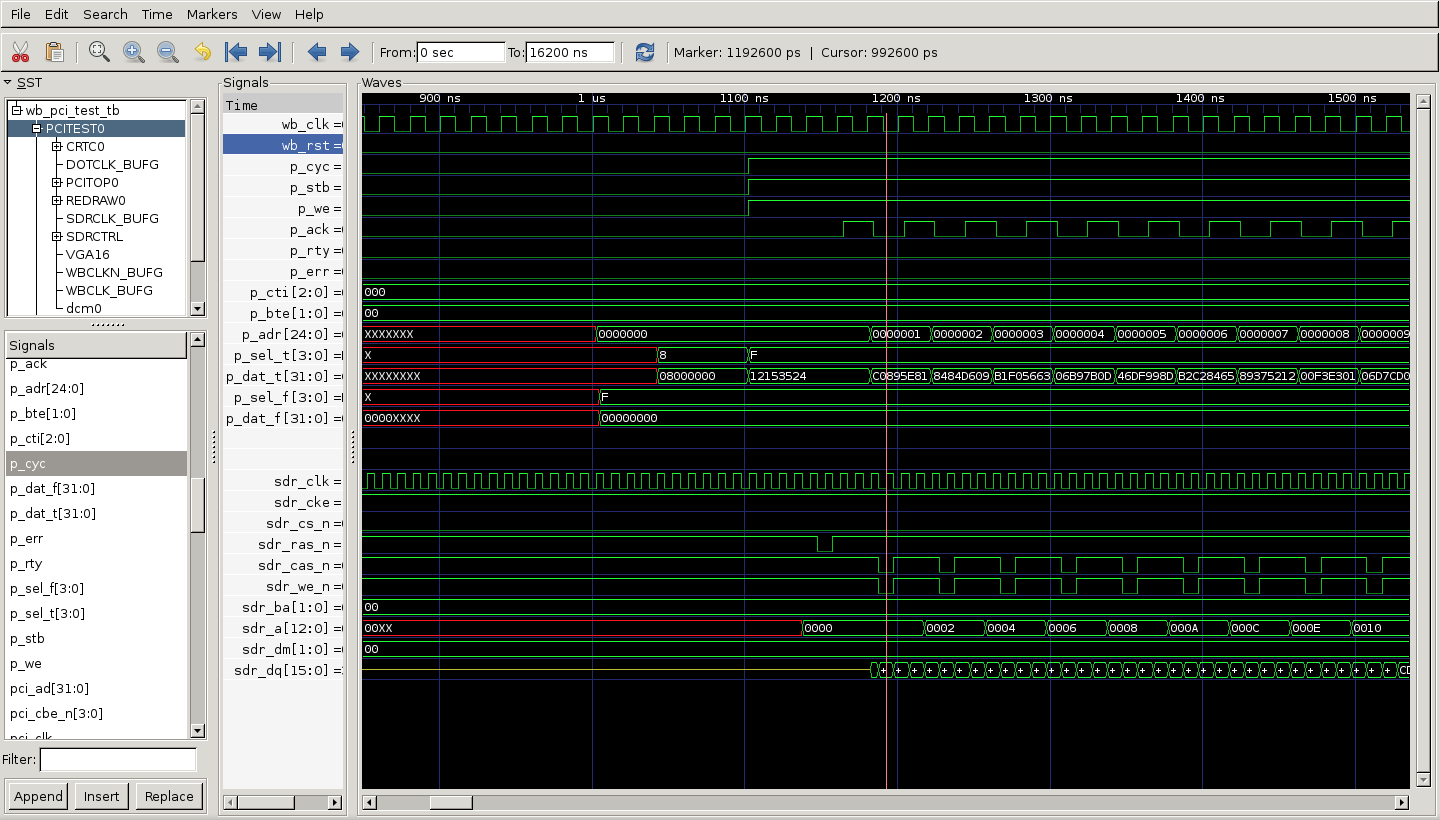
\includegraphics[width=\linewidth]{images/pci_to_sdram_xfer.pdf}
\caption[A simulation of a PCI to SDRAM data transfer]{A simulation of a PCI to
SDRAM data transfer.}
\label{MEM_GtkWave_SDRAM}
\end{figure}

Figure~\ref{MEM_GtkWave_SDRAM} is a GtkWave\footnote{GtkWave is free software and
is available from http://www.geda.seul.org/tools/gtkwave/index.html} screen
capture showing the simulation waveforms of a write-to-SDRAM transaction. The
transaction is initiated by the PCI bridge, transferred over the Wishbone bus to
the SDRAM controller. The SDRAM controller then writes this data to the SDRAM
device. This Wishbone bus transaction is a non-burst transfer (as determined by
the Wishbone signals \texttt{CTI} and \texttt{BTE}).

\begin{figure}[h!]
\begin{center}
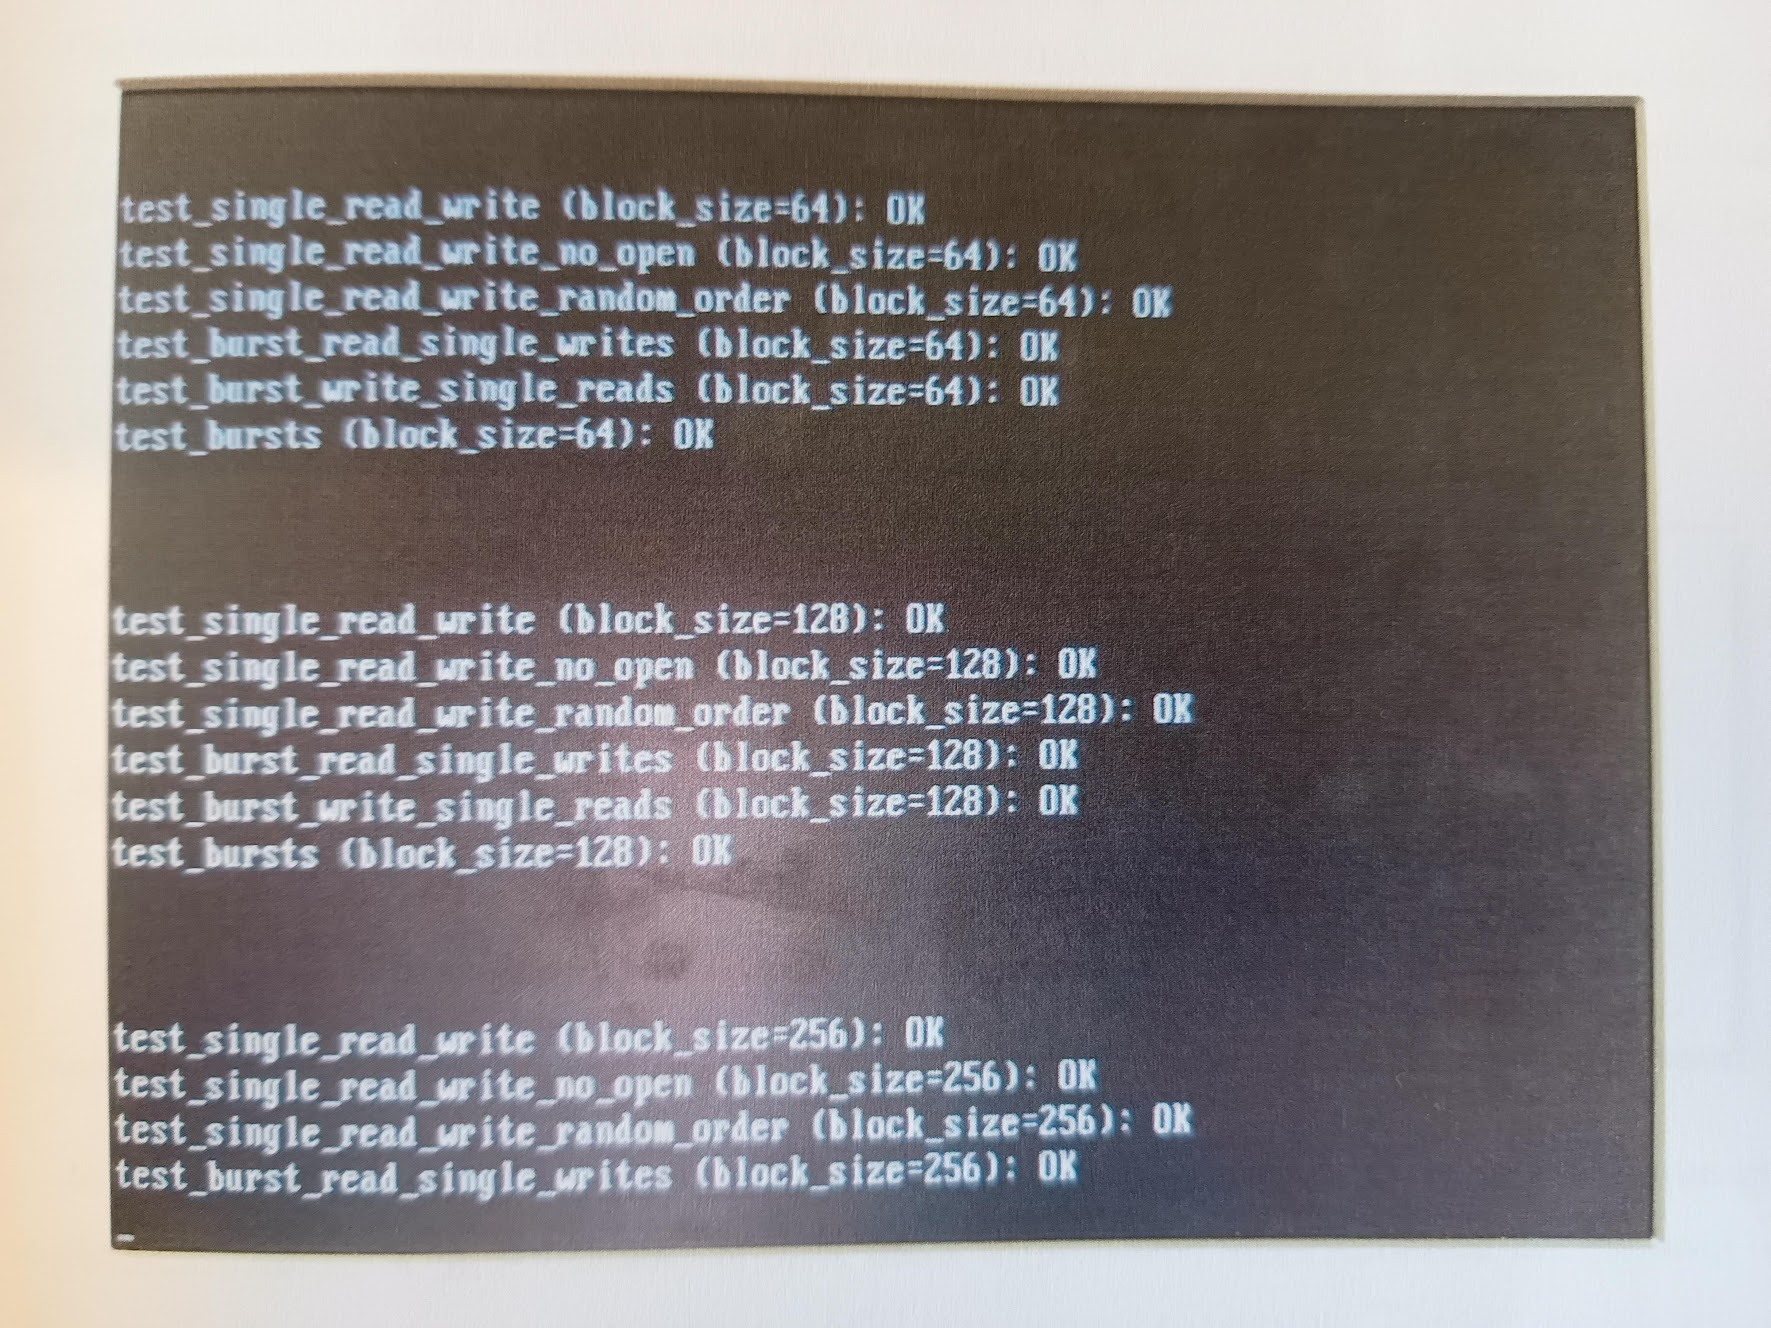
\includegraphics[width=\linewidth]{images/mem_test.jpeg}
\caption[SDRAM Memory Test Results]{OpenVGA passing memory tests
while running at 120 MHz.}
\label{MEM_Testing}
\end{center}
\end{figure}

A hardware testbench which only contained a subset of OpenVGA logic cores was
used when developing the SDRAM controller. A Linux kernel module for this
hardware testbench so that it could be accessed for testing using system API
calls. This module later became the OpenVGA kernel module.

The testing procedure consisted of writing blocks of data, of various block
sizes, and write orders, and with different transfer modes, and then reading back
and checking the data. The design passed memory tests without data corruption at
up to 120 MHz (see Figure~\ref{MEM_Testing}).


\subsubsection{Known Bugs}
\label{SDRAM_Bug}

There exists just one known bug with the SDRAM controller and this has been
narrowed down to a problem with write transactions. The system occasionally hangs
when performing large PCI burst-write transfers to OpenVGA. From the tests
performed, the following is known about this bug:

\begin{itemize}
  \item This bug is intermittent. There seems to be a small probability of it
  occurring for any PCI write transactions with a burst length of more than 256
  bytes.
  \item It occurred at all of the frequencies and memory timings tested, from
  25~MHz to 120~MHz, and with column address strobe latencies of 2, 2.5, and 3.
  \item Only occurs when the SDRAM controller logic core is used, other memory
  cores have not demonstrated this bug.
  \item It has only occurred during write operations, all reads seem unaffected.
  \item Changing the SDRAM refresh period seems to have no effect on the
  frequency of these hangs.
\end{itemize}

The system freeze does not occur when a Wishbone SRAM logic core is used instead,
indicating the problem is with the SDRAM controller, but all simulations have
failed to reproduce this bug, and hardware testing to date yields too little
information to locate the source of this bug. The current workaround is to use
many small burst transfers, rather than a few large ones.


\section{Data Cache}
\label{MEM_Cache}

\mmodule{Patrick Suggate}{wb\_simple\_cache}
{A Wishbone-compatible, 150 MHz, Spartan-3 optimised, 2 kB data cache which also
features a fast-hit lookup path.} {/rtl/cache/wb\_simple\_cache.v,
/rtl/cache/fetch\_wb.v, /rtl/cache/tag\_ram.v, /rtl/cache/cache\_bram.v}
{/sim/mem/wb\_sdram\_ctrl\_tb.v}{GPL}

A data cache for the OpenVGA processor was developed to significantly improve
memory access performance. A large quantity of data needs to processed when
updating the contents of the frame buffer, such as when performing ASCII text to
pixel conversion. The average latency of a single SDRAM memory access is high,
about 45 processor cycles per word read or written (see
Section~\ref{CACHE_Justification}), and the processor has to stall while waiting
for the memory controller.

So that the processor's memory access operations have a high throughput, low
average access latency is required. By using a data cache, average memory access
latency, and therefore performance, is improved by a factor of about eight for
the ASCII to pixel conversion algorithm (see Section~\ref{CACHE_Justification}).

The data cache has been designed to achieve a good compromise of the following
characteristics:
\begin{itemize}
  \item Logic resources used
  \item Clock frequency
  \item Design complexity
  \item Hit-time calculation
  \item Miss penalty
  \item Miss rate
\end{itemize}

For the sample workload, converting ASCII character data into pixel data, the
cache miss rate is extremely low (0.7\%), the clock rate high ($\approx$150
MHz), the average latency is only 5.1 clock cycles, and only about 80 Spartan-3
logic slices\footnote{Slice is the term Xilinx uses for its general purpose logic
resources, and within the Spartan-3 a slice contains a four-input Look-Up
Table\glossary{name={LUT}, description={Look-Up Table}} (LUT) and two DFFs}, and
a Block RAM, are used.


\subsection{Cache Justification}
\label{CACHE_Justification}
How much of an improvement in average Clock cycles required Per
Instruction\glossary{name={CPI}, description={Clocks Per Instruction}} (CPI) does
a data cache give? First, assuming OpenVGA is operating at screen resolution of
640x480, in 16-bit colour mode (2 bytes/pixel), and with a 60 Hz redraw, the data
rate ($r_\mathrm{RD}$) is given by

\[
r_\mathrm{RD} = 640 * 480 * 2 * 60 = 36864000~\mathrm{Bs}^{-1}
\]

The SDRAM controller operates at 50 MHz, the word size is 32-bits, the maximum
burst transfer size is 512 bytes, and the memory controller's fixed access
penalty (minimum memory access time, $t_\mathrm{MA}$) at 50 MHz is another eight
cycles for reads, or four cycles for writes. The parameter $t_\mathrm{MA}$ is
subsequently assumed to be six cycles per access for simplicity, though reads are
more frequent\footnote{Using six as the average penalty results in worse
statistics for the cache, so this is not an attempt to make the cache results
appear more impressive. Also, the DMA controller can be used for data writes with
ASCII text to pixel algorithm since it is well-behaved. This reduces memory bus
congestion.}.

The total redraw transaction rate ($r_\mathrm{RT}$) is given by

\[
r_\mathrm{RT} = \frac{r_\mathrm{RD}}{512} = \frac{36864000}{512} =
72000~\mathrm{Hz}.
\]

If a transaction requires $t_\mathrm{RD}$ cycles to complete, the sum of the
fixed and per-word transfer penalties, the total Wishbone bus cycles for 60
redraws, ($T_\mathrm{WB}$) is given by

\begin{eqnarray*}
T_\mathrm{WB} & = & r_\mathrm{RT} * t_\mathrm{RD} \\
  & = & 72000 * (128 + 8) = 9792000 \\
\end{eqnarray*}

Wishbone bus congestion ($c_\mathrm{WB}$), for the Wishbone bus frequency
($f_\mathrm{WB}$) of 50 MHz, is given by

\begin{eqnarray*}
c_\mathrm{WB} & = & \frac{T_\mathrm{WB}}{f_\mathrm{WB}} \\
 & = & \frac{9792000}{5\times10^7} \\
 & \approx & 20\%
\end{eqnarray*}

This result, $c_\mathrm{WB}$, is approximate because it does not have
prefetch-overshoot and refresh cycles factored in. Average memory access latency
is affected by ($c_\mathrm{WB}$). There is a probability of 0.2 that a memory
access will have to wait for a redraw prefetch transaction to complete. The
average wait is $\frac{1}{2}t_\mathrm{RD}$ cycles.

Average memory access latency ($l_\mathrm{WB}$) in Wishbone bus cycles is given
by

\begin{eqnarray*}
l_\mathrm{WB}	& = & \frac{1}{2}t_\mathrm{RD}\times 0.2 + t_\mathrm{MA} \times
0.8 \\
& = & 68 \times 0.2 + 6 \times 0.8 \\
& = & 18.4
\end{eqnarray*}

Additional parameters affecting the average memory access latency for the
processor ($l_\mathrm{CPU}$) are
\begin{itemize}
  \item $m_\mathrm{CPU}$: RISC16 has a CPU multiplier of two. This doubles
  the average memory latency seen by RISC16.
  \item $i_\mathrm{mem}$: RISC16 has a memory instruction latency cost of four
  additional cycles, due to the interlocking and flushing mechanism used.
  \item $t_\mathrm{sync}$: An additional synchronisation cost of four
  processor clock cycles because the processor and memory operate at different
  frequencies.
\end{itemize}
Giving $l_\mathrm{CPU}$ (in processor cycles)

\begin{eqnarray*}
l_\mathrm{CPU}	& = & l_\mathrm{WB} \times m_\mathrm{CPU} + i_\mathrm{mem} +
t_\mathrm{sync} \\
				& = & 18.4 \times 2 + 4 + 4 \\
				& \approx & 45
\end{eqnarray*}

Profiling the text-mode code shows that about 900,00 memory accesses (see
Figure~\ref{Mem_No_Cache}) which shows the total accesses for 50 such
conversions) are required for the conversion of a screen full of ASCII text data
to pixel data, (640x400 resolution, 16-bit colour).

If the desired display update rate, for the ASCII to pixel transformation, is 20
Hz, for smooth scrolling, and the cost for each of the memory accesses required
is 45 CPU cycles, then 720 million CPU clock cycles will be required per second.
The RISC16 processor will not be fast enough, it only operates at 100 MHz. If a
fast cache is used, which reduces average memory access time to about 5.1 cycles,
then the 100 MHz processor will be about fast enough.

% Additionally, since the average Wishbone transfer size will be larger, due to the
% DMA controller being used for memory writes, and also the number of transfers
% fewer, a data cache will result in reduced Wishbone bus congestion too. Using a
% DMA (see Section~\ref{MEM_DMA}) for writing to the SDRAM will only be more
% efficient when the write behaviour is well behaved. A large percentage of the
% entries within a cache line are modified, but since the text mode code is very
% sequential, this can safely assumed.
% 

\subsection{Implementation Considerations}
The Spartan-3 FPGA architecture has 2 kB BRAMs, which are built-in primitives,
and are suitable for implementing small caches. Each BRAM has two independent
ports and supports several different data widths. Due to the locations of the
BRAMs within the Spartan-3, aligned in two vertical columns on either side of the
FPGA, half in each column, two or more BRAMs can be connected in parallel to give
greater capacity, data transfer rates, and widths.

To design an efficient cache, the performance effects of set associativity, write
policy, capacity, data widths, line size, and replacement policy were examined.
The processor within OpenVGA has the primary purpose of converting data into a
format suitable for displaying, and for this particular application, memory
access consists of reading blocks of data, applying a transformation, and writing
the output to the framebuffer.

This sequential, block-reading/writing behaviour was speculated to heavily
benefit from a cache, since there is a high probability the next datum to be
read/written will be from one of the blocks currently cached. Furthermore, such
sequential behaviour should mean that small cache sizes will not reduce
performance much.

Factors responsible for performance when designing caches are:
\begin{itemize}
	\item Reducing the miss penalty.
	\item Reducing the miss rate.
	\item Reducing hit calculation time.
\end{itemize}
A cache that excels at all of these may well be too large to fit within the
200k-gate Spartan-3 FPGA used. To design a cache that gives good performance
without being too large, some objective measure of cache performance is needed.

Since designing and implementing a fast cache can also be very time-consuming, a
parameterisable cache simulator was written in C++ (see
Appendix~\ref{CODE_Cache}). This allows cache design parameters to be chosen
before the cache is constructed. Simply modifying the simulator parameters and
(re)running a test allows a different cache design to be evaluated. By
methodically changing each of the parameters, a cache has been chosen that will
perform well for the simulated task.

If an unrealistic simulation model is used for evaluating cache performance, due
to poor understanding of the problem, then the chosen parameters may not be
suitable for final cache design. The simulation model used for evaluating cache
performance was the ASCII text to pixel conversion algorithm, this was
implemented in C++ too (see Appendix~\ref{Source_Code}. The C++
implementation of this algorithm closely matches the desired characteristics of
the assembly routines that need to be written for the RISC16 or TTA16 processors.


\begin{figure}[h!]
\begin{center}
% \shadowbox{%
\Ovalbox{%
	\begin{minipage}{0.9\linewidth}
		\begin{center}
		\begin{minipage}{0.8\linewidth}

\begin{verbatim}

		Memory Statistics:
		Reads:		19280100
		Writes:		25684152
		Total:			44964252

		Total CPU memory access cycles: 2113319844 (Av: 47.0/op)

\end{verbatim}
		\end{minipage}
		\end{center}
	\end{minipage}}
\caption[Text-mode simulator without a cache]{Text-mode simulator output without
using a cache.}
\label{Mem_No_Cache}
\end{center}
\end{figure}

\begin{figure}[h!]
\begin{center}
\Ovalbox{%
	\begin{minipage}{0.9\linewidth}
		\begin{center}
		\begin{minipage}{0.8\linewidth}
\begin{verbatim}

Cache Properties:
    Cache Size:           2048
    Tags per Bank:          16
    Set associativity:   2-way
    Line (Block) Size:      64
    Write Policy:         thru

Memory Statistics:
Reads:		7812096
Writes:		28882131
Total:			36694227

Cache Statistics:
Accesses:	67364279
Hits:		67120151 (99.6%)
Fast Hits:	61714821 (91.9%)
Misses:		244128	(evicts = 0)
Miss rate(per 1000):	3.6

Total CPU memory access cycles:	358827429 (Av: 5.3/op)

\end{verbatim}
		\end{minipage}
		\end{center}
	\end{minipage}}
\caption[Text-mode simulator with a cache]{Text-mode simulator output when using
a cache.}
\label{Mem_With_Cache}
\end{center}
\end{figure}


\subsection{Set Associativity}
\label{CACHE_Associativity}
The set-associativity cache parameter represents how many cache look-up indices
are hashed from an incoming address. These indices are used to retrieve
cache-line tags for comparison with the incoming address. A cache with higher
set-associativity has a higher hit-rate, but also has larger and more complicated
cache sense logic.

A cache look-up consists of:
\begin{itemize}
  \item Hashing the incoming address to generate an index into the tag memory.
  \item Retrieving the tag from the tag memory.
  \item Comparing the tag-field of the incoming address to the retrieved tag.
  \item Signalling a hit and retrieving the data from cache upon a match, or
  else signalling that a miss has occurred.
\end{itemize}

With a direct-mapped cache, the incoming address can be hashed to only one
cache memory location, so there is only one tag to check. If the incoming
address is hashed to produce two different indices into the cache memory,
which data (if any) chosen depends on if either retrieved tag matches. Such a
cache design is said to be a two-way set associative cache. With two tag
banks, these two tag comparisons typically happen in parallel\cite{Comp_Arch}.

A fully associative cache requires that every tag be checked for a match. This
requires a lot of parallel comparison logic and tag memory bandwidth, and is
quite rare\cite{Comp_Arch}. Caches can be designed to be direct-mapped, or fully
associative, or anywhere in between these two extremes.

Fully associative caches typically have the highest hit
rates\cite{parhami2005cam}, if all other parameters held constant, since data can
be stored anywhere within the cache and the cache is free to choose any line to
evict. Direct-mapped caches have the lowest hit performance, but also the lowest
implementation cost (complexity, logic, and latency)\cite{Comp_Arch,
parhami2005cam}.

A two-way set associative cache was chosen since this is typically a good
trade-off for a small caches. It requires only one extra $n$-bit comparator and a
few extra logic gates, compared to a direct-mapped cache, and results in lower
miss-rates\cite{parhami2005cam}. A four-way set-associative cache would require
two more comparators than a two-way cache, and extra tag memories, and have a
higher latency on a Spartan-3 FPGA\footnote{The extra tag memories would be
needed because the Spartan-3 FPGA family has distributed RAMs with 16 entries. To
store the 32 tag entries, as determined later in this section, would require a
exactly two banks of distributed RAM for either a direct-mapped or two-way set
associative cache, but moving to a four-way set associative cache would require
two more banks of distributed memory, if simply to provide the required number of
memory read ports.}.



\subsection{Cache Size}
The results from simulating the text-mode redraw algorithm (see
Table~\ref{Mem_Cache_Size}) show that performance is extremely good with even
relatively small cache sizes because the total size of the read-data is quite
small, 2 kB of font data, 4 kB of text-mode frame buffer data, and some stack
reads.

\begin{table}[h!]
\begin{center}
% \begin{tabular}{| c | c | c | c | c |}
\begin{tabular}{ r  r  r  r  r }
% \hline
Cache & Lines   & Misses  & Miss Rate  & Average \\
Size  & (total) & (total) & (per 1000) & Latency \\
\hline
1 kB  &  16 & 485065 & 25.2 & 5.9 \\
2 kB  &  32 &  14255 &  0.7 & 5.1 \\
4 kB  &  64 &   2633 &  0.1 & 5.1 \\
8 kB  & 128 &     97 &  0.0 & 5.1 \\
16 kB & 256 &     97 &  0.0 & 5.1 \\
% \hline
\end{tabular}
\caption[Cache size vs. performance]{Performance effects of different cache
sizes, with a two-way set associative, 64 byte line size, write-through cache.}
\label{Mem_Cache_Size}
\end{center}
\end{table}

Based off these results, 2 kB, the size of a Spartan-3 BRAM, appears to be a good
choice. There is little advantage, FPGA resource usage-wise, for going smaller.
With sizes greater than 2 kB there is no significant average latency improvement,
and the extra complexity and resource usage of larger caches is of minimal
benefit in this application.


\subsection{Cache Line Size}
Shorter lines for a given size of cache require more entries within the cache
lookup table. Longer cache-lines mean that more data has to be fetched from main
memory, but the hit rate for subsequent sequential accesses will be higher.

\begin{table}[h!]
\begin{center}
\begin{tabular}{r r r r}
Line Size & Lines   & Miss Rate  & Average \\
 (bytes)  & (total) & (per 1000) & Latency \\
\hline
8   & 256 & 1.9  & 5.2 \\
16  & 128 & 1.2  & 5.2 \\
32  & 64  & 0.8  & 5.1 \\
64  & 32  & 0.7  & 5.1 \\
128 & 16  & 1.1  & 5.2 \\
256 & 8   & 3.4  & 5.4 \\
\end{tabular}
\caption[Cache line-size vs. performance]{Performance effects of different
cache line sizes, with a two-way set associative, 2 kB, write-through cache.}
\label{MEM_Line_Size}
\end{center}
\end{table}

The 2 kB data cache demonstrates excellent performance with all tested line-sizes
(see Table~\ref{MEM_Line_Size}), but the number of tags to store doubles as the
line-size halves, for a given cache size. Since a single Spartan-3 distributed
RAM has 16 entries, and there are two tag banks within a two-way set associative
cache, this means that a line size of 64~bytes is the most efficient hardware
implementation, as well as having a slight performance edge. A line size of
64~bytes was chosen for the final cache.


\subsection{Replacement Policy}
To determine which cache line to evict on a data miss, three cache data
replacement policies were evaluated:
\begin{itemize}
 \item Least Recently Used (LRU)
 \item First In, First Out (FIFO, also called round-robin)
 \item Random
\end{itemize}

Results from the cache simulator (see Figure~\ref{Mem_OpenVGA_Evict_Policy})
agreed with published results for simulations done with an Alpha 21264
processor\cite{Comp_Arch} (see Table~\ref{Mem_Alpha_Evict_Policy}).

\begin{table}[h!]
\begin{center}
% \begin{tabular}{| c | c | c | c |}
\begin{tabular}{r r r r}
% \hline
Size & LRU & Random & FIFO \\
\hline
16 kB & 114.1 & 117.3 & 115.5 \\
64 kB & 103.4 & 104.3 & 103.9 \\
256 kB & 92.2 & 92.1 & 92.5 \\
% \hline
\end{tabular}
\caption[DEC Alpha 21264 cache eviction policy vs. performance]{Different
cache eviction policies, with a two-way set associative cache, and their effect
upon cache miss rate, per 1000 instructions, with a DEC Alpha 21264 processor
running the SPEC2000 benchmarks\cite{Comp_Arch}.}
\label{Mem_Alpha_Evict_Policy}
\end{center}
\end{table}

\begin{table}[h!]
\begin{center}
\begin{tabular}{l r r}
Replacement Policy & Miss Rate & Average \\
 & (per 1000) & Latency \\
\hline
Least Recently Used & 0.8 & 5.1 \\
Random & 0.7 & 5.1 \\
First-In, First-Out & 0.8 & 5.1 \\
\end{tabular}
\caption[Cache eviction policy vs. performance]{Different cache replacement
policies and the effect on miss-rates and average latencies when simulated
using the text-mode redraw algorithm and a 2 kB, two-way set associative, 64
byte line size, write-through, data cache.}
\label{Mem_OpenVGA_Evict_Policy}
\end{center}
\end{table}

Random replacement was therefore chosen since it is the easiest to implement. The
random replacement selector is a single bit of a seven bit LFSR, as LFSRs have
been shown to generate good approximations of random
sequences\cite{dufaza1991lbd}.


\subsection{Write Policy}
The two approaches with writes to the cache are to attempt to write it straight
away (the write through policy), or store incoming data in the cache so that it
can be written to the memory in bursts. The second approach, the write back
policy, was less efficient in this case (see Table~\ref{Write_Policy}), and is
more complex to implement, so the data cache uses write though instead.

Since the majority of data written with the cache simulator, and simulating the
text to pixel conversion algorithm, uses writes to the DMA controller, not direct
memory writes, the performance of each approach will not have a significant
effect in this case anyway.

\begin{table}[h]
\begin{center}
% \begin{tabular}{| c || c | c || c | c |}
\begin{tabular}{r | r r | r r }
% \hline
Line Size & Write Back & & Write Through & \\
(bytes) & Misses/1000 & Cycles/Op & Misses/1000 & Cycles/Op \\
\hline
8   &  75.0 &  8.7 & 1.9 & 5.2 \\
16  &  37.9 &  7.1 & 1.2 & 5.2 \\
32  &  19.3 &  6.3 & 0.8 & 5.1 \\
64  &  10.9 &  6.0 & 0.7 & 5.1 \\
128 &   9.5 &  6.2 & 1.1 & 5.2 \\
256 &  20.2 &  8.6 & 3.4 & 5.4 \\
% \hline
\end{tabular}
\caption[Cache Write Policies vs. Performance]{Different cache write policies
and line-sizes, with a 2 kB, two-way set associative cache, and their effect
upon average memory latency, and cache miss rate per 1000 instructions.}
\label{Write_Policy}
\end{center}
\end{table}


\subsection{Pipeline Length}
\label{CACHE_Pipeline}
The data cache interface to the processor needs to run at the processor frequency
to minimise latency but, since hit calculation (performed by the sense logic)
requires cache tag lookup and then address comparison, there is a large
combinatorial delay, so this logic was pipelined.

\begin{figure}[h!]
\begin{center}
\includegraphics[width=\linewidth]{diagrams/cache_sense_logic.pdf}
\caption[Simplified Schematic of the Cache Sense Logic]{Simplified schematic
showing the cache sense logic.}
\label{CACHE_Sense}
\end{center}
\end{figure}

The previous two tags used for a cache look-up operation are stored so if the
same cache tag index is subsequently used, the look-up operation will take one
less clock cycle. These are called ``Fast Hits'' in the cache simulator output,
and this was about 90\% of all hits with the cache simulations, so the average
latency saving from this optimisation is about 0.9 cycles per memory access. The
previous-tag registers have an additional purpose as well. Since tag retrieval
takes several nanoseconds, they are used as pipeline registers so the cache can
operate at a higher clock frequency.

Upon hit, the total latency is zero cycles for a fast hit and one cycle for a
normal cache hit. The miss latency is determined by the state of the SDRAM as
well as the overhead imposed by the cache, plus the signal synchronisation, in
each direction, since the memory access crosses from the processor domain
to the Wishbone bus domain and back. Minimum total latency for a read is 15
cycles plus an additional one quarter of the line size (and the processor
design adds another five), but average latency for a miss will be a lot higher
since the video redraw logic is competing for SDRAM access too.

Figure~\ref{CACHE_Sense} is a simplification the data cache sense logic. The
Wishbone signals used to initiate a cache look-up are shown on the left
(\texttt{CYC}, \texttt{STB}, \texttt{WE}, and \texttt{ADR}). The \texttt{Miss}
signal is used to initiate a fetch from memory and is only asserted by cache-read
misses, never for cache-writes. The \texttt{Hit} signal is used to complete a
cache look-up transaction.


\subsection{Testing}
The first part of testing the cache was building a software cache simulator. This
allowed evaluating changes to the design can be made quickly and the performance
implications simulated and evaluated. A text-mode conversion algorithm was
written in as well. This was used with the cache simulator to provide a realistic
test scenario, and the CRT simulator was used to verify correctness.

To hardware-test the synthesised cache, software writing to OpenVGA using
PCI-to-Wishbone bridge logic core provided a workload for the cache. All PCI
bridge transactions had to pass through the cache to access the SDRAM, and the
same memory-test applications that were written for the SDRAM controller (see
Section~\ref{MEM_Testing}) could be used.



\section{DMA Controller}
\label{MEM_DMA}

\mmodule{Patrick Suggate}{wb\_dma}
{A DMA controller for writing data in bursts to a memory controller.}
{/rtl/lib/wb\_dma.v} {/sim/lib/wb\_dma\_tb.v}{GPL}

The DMA allows a peripheral to queue up write data so that it can be written to
the memory controller as a burst transfer, improving total system memory
throughput. The DMA consists of a FIFO, using a 2 kB BRAM, to buffer data until
it is ready to be written. If the DMA has been filled with 2 kB of data, it can
optionally be re-written multiple times to any location in memory. This is useful
for clearing the OpenVGA display memory for example. Information on how to access
and program the DMA controller is contained in Section~\ref{TTAPROG_DMA} of the
TTA16 programming guide.


\section{Serial PROM}
\label{Serial_PROM}

\mmodule{Patrick Suggate}{wb\_sprom}
{A Wishbone-compatible, serial PROM read-back module designed to work with Xilinx
serial PROMs.} {/rtl/lib/wb\_sprom.v} {/sim/lib/wb\_sprom\_tb.v}{GPL}

Since the FPGA state is stored internally, using SRAM, it needs to be reloaded
every time the device is powered on. Xilinx sell a Serial Flash PROM to
accomplish this task. After the initial FPGA state is loaded from this PROM,
the user can then access the PROM and read out additional data.

When building the binary image file for the PROM contents, extra data can be
appended to the end of the PROM image file. This requires some padding
bytes and an ID pattern preceding the appended data. This can then be read back
once the FPGA performs its own initialisation.

The serial PROM is needed to store the VGABIOS ROM image and additional
processor instructions, which is transferred to SDRAM upon start-up. The VGABIOS
ROM image is 32 kB of 16-bit, x86 code which resides at address 0x0C8000 in the
OpenVGA host computer's memory address space\cite{SVGA_Book}. The purpose of
this ROM is too implement standard routines for communicating with the VGA hardware.


\subsection{Serial PROM Read-Back Considerations}
Since this is typically done only on power-on, since sequential access without
direct control of the address counter is very slow, the PROM read logic should
be small so to minimise logic usage for hardware that is used just once.

The simplest way to read data from this serial PROM is to clock the data out
into a shift register, searching first for the ID pattern to locate the
beginning of user data, then continue clocking while transferring the user data
onto the Wishbone bus and to the SDRAM.

\chapter{I/O Logic Cores and Data Synchronisation}
\label{IO_Chapter}

This chapter describes the logic cores used to communicate with the PCI Local
Bus, the video DAC, the DVI TMDS encoder, the USB UART, and the LEDs. Also
contained is the clocking and data synchronising issues that had to be solved so
that the previously mentioned logic cores can exchange data using the OpenVGA
Wishbone bus.


\section{Clock Architecture}
\label{CLOCK}
All OpenVGA clock signals are derived from either the 33~MHz PCI clock, or the
50~MHz on-board crystal oscillator (see Figure~\ref{OPENVGA_OpenVGA}). The
display dot-clock, while derived from the 50~MHz oscillator, has to be treated as a
separate clock domain since its frequency can be set to either 25~MHz or 40~MHz,
depending on the video mode.


\subsection{Spartan-3 Clocking Resources}

The Spartan-3 contains low-skew clock lines which can be connected to all the
logic resources within the FPGA. To drive these lines there are a couple of logic
primitives, \texttt{BUFGMUX} and \texttt{DCM}, that can be used.


\subsubsection{Global Clocks}

\mmodule{Patrick Suggate}{BUFGMUX, BUFG}
{Simulation modules which emulate the functionality of the Xilinx Spartan-3
primitives with the same name.} {/sim/xilinx/BUFGMUX.v, /sim/xilinx/BUFG.v}
{/sim/xilinx/BUFGMUX\_tb.v, /sim/xilinx/BUFG\_tb.v}{GPL}

The 200k-gate Xilinx Spartan-3 FPGA has eight dedicated, low-skew, global clock
lines~\cite{Xilinx_SP3_DS}. These are routed throughout the FPGA and designed
primarily for use as clock and reset signals. Skew on the clock or reset signals
can cause metastability so it is essential that skew on these lines is low, or at
least known. XST automatically calculates the skew of a synthesised design, and
generates a timing report for the clock signals. These reports also include
warnings when a design uses clock signals in a way that may cause unpredictable
skew.

Clock signals can be explicitly routed into global clock lines using the Xilinx
\texttt{BUFGMUX} primitive, though this is normally performed automatically by
XST. A \texttt{BUFGMUX} is a two input multiplexer and the output is a global
clock line. This primitive allows one of two different clock signal inputs to be
selected as the source. This primitive contains logic to avoid clock glitches so
the input source clock can be dynamically switched.


\subsubsection{Digital Clock Managers}
\label{CLOCK_DCM}

\mmodule{Patrick Suggate}{DCM}
{Simulation modules which emulate the functionality of the Xilinx Spartan-3
primitives with the same name.} {/sim/xilinx/DCM.v} {/sim/xilinx/DCM\_tb.v}{GPL}

The Spartan-3 family of FPGAs typically contain four DCM (Digital Clock Manager)
primitives, except for the smallest device which only has
two~\cite{Xilinx_SP3_DS}. DCMs use DLLs (Delay-Locked Loops) to condition clock
input signals, and optionally phase-shift and derive new clocks as well.
Conditioning the input clock signals ensures a clean clock output, corrects the
duty-cycle (optional), and allows XST to more accurately assess and control
clock-skew. Additionally, the input clock period can be multiplied and divided to
generate new clocks, and this feature was used to generate processor, SDRAM, and
VGA clocks from the on-board 50~MHz oscillator.

\begin{figure}[h!]
\begin{center}
\includegraphics[width=0.65\linewidth]{diagrams/bufgmux.eps}
\caption[OpenVGA pixel clock generation]{BUFGMUX and DCM example showing the
OpenVGA pixel clock generation.}
\label{CLOCK_BUFGMUX}
\end{center}
\end{figure}

%  using a BUFGMUX. The pixel clock can be selected as one of two DCM outputs. The DCM has
% an optional divide-by-two parameter to halve the input clock if needed, so the
% CLK0 output is 25 MHz, and the CLKFX signal is set to output 40 MHz for use with
% the 800x600 resolution video mode

\subsection{Clock Domains}

The operating frequency of the PCI Local Bus is nominally~33 MHz~\cite{PCI_Book},
but this is not certain. There are PCI power saving modes in which the bus
frequency can be lowered, possibly even to zero\footnote{In addition,
off-the-shelf motherboard's PCI system clock can differ significantly from the
specification as the PCI clock is often derived from the Front Side Bus (FSB)
clock, which can be adjusted by the user, or differ due to manufacturing
tolerances.\cite{PCI_Book}}, for example. The video DAC and TMDS encoder ICs
operate at the dot-clock frequency, 25~MHz for the 640x480 resolution VGA. Since
these clocks differ, and also differ from the 50~MHz Wishbone bus clock, data
crossing these separate domains need to be synchronised.

The Spartan-3 FPGA has clocking resources which support clock generation and
conditioning, and multiple clock signals~\cite{SP3_DCM}. The is also logic
primitives suitable for constructing asynchronous FIFOs, a logic core used to
transfer data between clock domains.


\begin{table}[h!]
\begin{center}
\begin{tabular}{l | c c r c | c}
Clock Name & \multicolumn{4}{c|}{Clock Frequency} & Domain	\\
& \multicolumn{4}{c|}{(MHz)} & Name	\\
\hline
Wishbone Clock			& & & 50	& & Wishbone \\
CPU Clock (RISC16)		& & & 100	& & \\
CPU Clock (TTA16)		& & & 150	& & \\
SDRAM Controller Clock	& & & 50	& & \\
SDRAM Datapath Clock	& & & 100	& & \\
\hline
Video Clock 0 (640x480)	& & & 25	& & Dot Clock\\
Video Clock 1 (800x600)	& & & 40	& & \\
\hline
PCI Local Bus Clock		& & & 33	& & PCI \\
\end{tabular}
\end{center}
\label{CLOCK_Frequencies}
\caption[OpenVGA clock frequencies]{OpenVGA's clock domains and
frequencies.}
\end{table}

OpenVGA has multiple, asynchronous clock domains (see
Section~\ref{CLOCK_Async_Domains}, and data needs to be transferred between clock
domains. To prevent problems due to metastability\footnote{A full discussion of
metastability is beyond the scope of this work but a D flip-flop can enter a
metastable state if setup and/or hold times are violated. Its data output can
become essentially random.}, data crossing asynchronous clock domains needs to be
synchronised. A single-bit synchroniser is shown in Figure~\ref{CLOCK_Synchro},
and for signals many bits wide, asynchronous FIFOs (see
Section~\ref{CLOCK_Async_FIFO}) are used for synchronisation.


\subsubsection{Synchronous Clock Domains}
\label{CLOCK_Sync}

\mmodule{Patrick Suggate}{wb\_sync}
{Synchronises Wishbone transactions between two Wishbone buses with synchronous,
but different frequency, clocks.} {/rtl/lib/wb\_sync.v}
{/sim/lib/wb\_sync\_tb.v}{GPL}

Data is transported between separate OpenVGA functional units, internal to the
Spartan-3, via a Wishbone compatible bus (see Appendix~\ref{APP_Wishbone}). The
Wishbone bus clock is 50 MHz and is the DCM conditioned output generated by the
50 MHz on-board oscillator.

The CPU, SDRAM datapath, and the pixel clock, all share a common
root clock, the 50 MHz Wishbone bus clock. Though different frequencies are
used for each, the CPU (see Chapter~\ref{CPU}) and SDRAM controller (see
Section~\ref{MEM_SDRAM}) clocks are synchronous with the Wishbone bus clock,
and with frequencies that are integer multiples of the Wishbone bus clock
frequency (see Table~\ref{CLOCK_Frequencies}).

\begin{figure}[h!]
\begin{center}
\fbox{
\begin{minipage}{0.9\linewidth}
\begin{center}

\begin{tabular}{c c}
\multicolumn{2}{c}{Synchronisers for single-bit signals crossing between
different clock domains}\\
\\
Synchronous & Asynchronous	\\
\includegraphics[width=0.33\linewidth]{diagrams/synchroniser.eps}	&
\includegraphics[width=0.44\linewidth]{diagrams/sync2.eps}
\end{tabular}
\end{center}
\end{minipage}
}
\end{center}

\caption[Single-bit synchronisers]{A synchronisers for crossing clock domains.}
\label{CLOCK_Synchro}
\end{figure}

Transitions between these synchronous clock domains requires two DFFs (see
Figure~\ref{CLOCK_Synchro}) for each signal that crosses a domain boundary.
Additionally, signals multiple bits wide retain the same relative phase when
crossing synchronous domains using simple synchronisers, which is not the case
for crossing asynchronous domains using simple synchronisers\cite{Async_FIFO}.


There are three additional problems when crossing synchronous clock domains:
\begin{enumerate}
\item A signal crossing from the higher-frequency domain, to the slower domain, needs
to be asserted for at least one cycle of the slower clock so it is registered
correctly.
\item  When a signal crosses from the slower clock domain, to the higher frequency
clock domain, the higher frequency domain needs to correctly handle that the
signal might remain asserted for more than one cycle of the faster clock, but
should only trigger once.
\item At the boundary of two synchronous signals, the setup and hold times must
be met for both D flip-flops, which means that the smallest period of the two
timing constraints has to be applied to both DFFs.
\end{enumerate}

To solve the first two of these issues, an acknowledge (ACK) signal was used
when crossing synchronous clock domains. This indicates that a signal has been
correctly registered. The signal source then de-asserts the signal at the end of
the cycle which the ACK was received. For the final problem, XST automatically
applies the correct constraint but the designer still needs to be aware that
the tightest of the two constraints will apply to any combinatorial logic.


\subsubsection{Asynchronous Clock Domains}
\label{CLOCK_Async_Domains}
To cross asynchronous clock domains there are two common methods: a simple two
flip-flop synchroniser (see Figure~\ref{CLOCK_Synchro}), which is useful for
single bit flags like an interrupt signal; and asynchronous FIFOs, which are
useful for multiple bit-width signals, like buses, where a phase relationship
has to be maintained for all signals, across the entire width~\cite{Async_FIFO}.

\subsection{Asynchronous FIFOs}
\label{CLOCK_Async_FIFO}

\mmodule{Patrick Suggate}{afifo16, afifo2k}
{Parameterisable, asynchronous FIFOs, with either 16 or 2048 entries, which
synchronise and queue data which has to cross asynchronous clock domains.}
{/rtl/lib/fifo/afifo16.v, /rtl/lib/fifo/afifo2k.v, /rtl/lib/counter/bin2gray.v}
{/sim/lib/wb\_sync\_tb.v}{GPL}

% \begin{tabular}{l l}
% \textbf{Modules:}		& afifo16, afifo2k	\\
% \textbf{Related Files:}	& /rtl/lib/fifo/afifo16.v, /rtl/lib/fifo/afifo16.v, 	\\
% 						& /rtl/lib/counter/bin2gray.v	\\
% \textbf{Testing Files:}	& /sim/lib/fifo/afifo\_tb.v	\\
% \end{tabular}

An asynchronous FIFO takes write data from one clock domain and stores it
internally within a queue, implemented using SRAM, and the data can then be read
out to the other clock domain. The FIFO generates control signals to indicate its
state (empty, full, etc.) so that data is not written to a full FIFO, or
requested from an empty FIFO. To avoid metastability, even these control signals
are valid in just one domain. Typically the empty signal is valid in the FIFO's
read clock domain, and the FIFO's full signal is typically valid within the
FIFO's write clock domain.

The penalty due to having to use an asynchronous FIFO is both a latency penalty
and extra logic usage (approximately 60 Spartan-3 logic slices per 32-bit wide
FIFO, see Section~\ref{CLOCK_FIFO_Synth}). Asynchronous FIFOs are only used for
the PCI and the video redraw circuits since each are within separate asynchronous
clock domains.

There are two logical divisions of the design for an asynchronous FIFO: the logic
for adding data to the FIFO, and removing data from the FIFO; and the logic for
comparing the read and write pointer values across clock domains to allow the
setting of FIFO state flags.

\begin{figure}[h!]
\begin{center}
\includegraphics[width=\linewidth]{diagrams/afifo.eps}
\caption[Simplified Asynchronous FIFO Schematic]{Simplified schematic showing
the basic components of an asynchronous FIFO.}
\label{FIFO_Logic}
\end{center}
\end{figure}

The logic for adding (and removing) data is straightforward, simply increment the
write pointer every time data is added, and increment the read pointer whenever
data is removed. Figure~\ref{FIFO_Logic} is a simplified diagram of a FIFO, the
Gray-encoders are not shown, and neither is a faster \texttt{full} and
\texttt{empty} assertion path. These are covered in detail in~\cite{Async_FIFO2}.

Comparing these pointers across clock domains, as is needed to set the
full and empty flags, is more difficult due to the possibility of
metastability. Standard base-2, ripple-carry incrementers can have multiple,
even all, bits change during an increment operation. This could potentially
cause every bit to become non-deterministic within the post-synchronised,
pointer representation.

The first step for the control signal generation is to convert the pointers into
a unit-distance representation\footnote{A unit distance encoding means that only one
bit changes between successive values in a sequence, but arithmetic in this
encoding is more complex which is why a standard representation is used for the
pointers.}, like Gray encoding, and this was used here (see
Table~\ref{CLOCK_Gray_Codes}. Even with metastability the desired pointer value
has a maximum difference of one from any generated post-synchronised pointer.
The only two values that the post-synchronised pointer can have is the previous
value or the desired value, and this will become the correct value the
following clock cycle anyway~\cite{Async_FIFO, Async_FIFO2}.

\begin{table}
\begin{center}
\begin{tabular}{| r || r | r |}
\hline
Decimal & Binary & Gray Code \\
\hline
0 & 0000 & 0000 \\
1 & 0001 & 0001 \\
2 & 0010 & 0011 \\
3 & 0011 & 0010 \\
4 & 0100 & 0110 \\
5 & 0101 & 0111 \\
6 & 0110 & 0101 \\
7 & 0111 & 0100 \\
8 & 1000 & 1100 \\
9 & 1001 & 1101 \\
10 & 1010 & 1111 \\
11 & 1011 & 1110 \\
12 & 1100 & 1010 \\
13 & 1101 & 1011 \\
14 & 1110 & 1001 \\
15 & 1111 & 1000 \\
\hline
\end{tabular}
\caption[Comparison of Decimal, Binary, and Gray Encoding.]{Gray codes with the
standard binary and decimal equivalents.}
\label{CLOCK_Gray_Codes}
\end{center}
\end{table}


\subsubsection{Control Signals}
Either the \texttt{full} or \texttt{empty} signals are asserted when the two
Gray-encoded counters match. Depending whether the the match was caused by the
FIFO going full, or going empty, determines which of the two flags is asserted.

The count order of the two Most Significant Bits\glossary{name={MSB},
description={Most Significant Bit}} (MSBs) of a Gray code counter are identical
to the two MSBs of the standard binary encoding. By sampling the two MSBs of the
Gray codes we can determine which quadrant the value is in. Using this quadrant
detection, and by comparing the current pointer values with the previous pointer
values, it can be determined whether the FIFO was going full, or going empty,
immediately before the pointers matched.


\subsubsection{Half-Full Detection}
In some applications, as with the video redraw circuit, it is useful to prefetch
multiple words, since this makes more efficient use of the Wishbone bus. Before a
prefetch is issued the prefetch control logic needs to know whether there is
space in the FIFO for the entire data transfer. An extra FIFO control signal,
calculated by comparing pointer quadrants, was added for this purpose.

By comparing the two MSBs of the FIFO read and write pointers, since these
quadrant bits have the same value as the standard binary encoding, the FIFO can
calcualte the difference in quadrants between the two pointers. If the quadrant
bits are equal then both pointers are within the same quadrant so the FIFO is
less than $25\%$, or more than $75\%$ full. If there are more than two quadrants
between the write and the read pointer, then the FIFO can also more than three
quarters full. The result is a control signal that detects whether the FIFO is
between $25\%$ and $75\%$ full (or not), and has been labelled \texttt{halfish}.


\subsubsection{Performance and Size}
\label{CLOCK_FIFO_Synth}

The size of a synthesised asynchronous FIFO, with a data width of 32-bits, and
with the target a Xilinx Spartan-3 FPGA was 59 slices\footnote{The 200k gate
Spartan-3 device that was used for OpenVGA contains 1920 logic slices}. With high
optimisation settings, the maximum speed at which the FIFO clocks is 144~MHz,
with the data write clock domain being the slowest (clock period of 6.9~ns). The
read clock domain achieved a clock period 3.8~ns, but since the logic for both
domains is very similar, this difference was speculated to be due to how XST
optimised the design.


\section{PCI-to-Wishbone Bridge}
\label{PCI}

\mmodule{Patrick Suggate}{pci\_mem\_top}
{A \textit{Plug and Play} compliant PCI-to-Wishbone-bridge logic core.}
{/rtl/pci/pci\_mem\_top.v, /rtl/pci/pci\_mem.v, /rtl/pci/cfgspace.v}
{/rtl/pci/pci\_mem\_top\_tb.v}{GPL}

OpenVGA connects to the host computer using the Peripheral Component Interconnect
(PCI) Local Bus. All data exchanged between OpenVGA and the host is through the
PCI-to-Wishbone bridge logic core. PCI was developed by Intel in 1991 as a
replacement for the aging Industry Standard Architecture (ISA)
Bus~\cite{PCI_Book, PCI_Spec}. PCI features data widths of 32 or 64 bits and has
nominal operating frequencies of 33 or 66 MHz (but can be reduced by power saving
modes).

\begin{figure}[h!]
\begin{center}
\includegraphics[width=\linewidth]{images/pci_bridge.eps}
\end{center}
\caption[PCI-to-Wishbone bridge block diagram]{PCI-to-Wishbone bridge block
diagram.}
\label{PCI_Block_Diagram}
\end{figure}


\subsection{PCI-to-Wishbone Bridge Logic Core}
This logic core maps OpenVGA's local memory into the host-system's address space,
and this bridge allows data to pass between the host and OpenVGA.
Figure~\ref{PCI_Block_Diagram} represents a simplified diagram of this logic
core. The OpenVGA PCI bus interface is in a separate clock domain to the system
Wishbone bus. PCI typically operates at 33 MHz, with the clock signal provided by
the host system, and the Wishbone bus domain operates at 50 MHz. This clock is
generated using an on-board crystal oscillator.

The PCI bridge logic core consists of two state machines, two asynchronous FIFOs,
and some additional control and pipelining logic. Asynchronous FIFOs were used so
that data can be transferred from one clock domain to another (see
Figure~\ref{PCI_Block_Diagram}). When synchronising signals across clock domains,
these FIFOs typically add a latency penalty of two clock cycles. Domain crossing
therefore adds two cycles of latency for a PCI write and four cycles of latency
for a PCI read request.


\subsubsection{PCI-Domain State Machine}
This state machine queues PCI read and write requests, and write data, in the
PCI-to-Wishbone asynchronous FIFO. PCI read transactions require that data be
fetched from the Wishbone bus domain and placed in the Wishbone-to-PCI FIFO. The
contents of this FIFO can then be read from the PCI domain, with the data being
placed on the PCI bus. The states of this state-machine, and the signals that
cause transitions between these states, are shown in Figure~\ref{PCI_SMs}.

To prevent the PCI bridge from being overwhelmed by many back-to-back PCI write
transactions, the bridge will generate \texttt{TARGET ABORT} responses when the
bridge is already busy. Multiple PCI read requests cause no problems though. This
is because they must wait for data retrieved from the Wishbone domain before
the transaction is completed.

\begin{figure}[h!]
\begin{center}
\includegraphics[width=\linewidth]{images/pci_state_machines.eps}
\end{center}
\caption[The PCI bridge state machines]{The PCI bridge state machines.}
\label{PCI_SMs}
\end{figure}

% The \texttt{wb{\_}busy} signal indicates there are pending writes, stored in the
% FIFO, so a PCI \texttt{TARGET ABORT} command is issued to terminate the current
% transaction, to be retried later. While in the \texttt{IDLE} state, if a PCI
% transaction is intiated by a PCI master, the address is stored in the
% PCI-to-Wishbone FIFO. \\
% In the \texttt{READ} state, any 32-bit words in the Wishbone-to-PCI FIFO are
% transferred to the PCI bus, and asserting the \texttt{TARGET READY} signal to
% indicate valid data. \\
% In the \texttt{WRITE} state, data is retreived from the PCI bus and stored in the
% PCI to Wishbone FIFO, as space allows. For every 32-bit word transfered to the
% FIFO \texttt{TARGET READY} is asserted.


% \begin{figure}[h!]
% \begin{center}
% \includegraphics[width=\linewidth]{diagrams/pci_pci_state_machine.eps}
% \end{center}
% \caption[PCI clock domain state machine]{PCI clock domain state machine.}
% \label{PCI_PCI_SM}
% \end{figure}


\subsubsection{Wishbone-Domain State Machine}
The PCI-to-Wishbone FIFO's \texttt{empty} signal de-asserting indicates that
there is a PCI request pending. The Wishbone-side state machine decodes this
request and issues a corresponding Wishbone transaction. Reads result in data
being transferred to the PCI domain using the Wishbone-to-PCI asynchronous FIFO,
writes use the PCI-to-Wishbone FIFO to transfer data to the Wishbone domain.

Summary of this state's machines signals:
\begin{itemize}
  \item \texttt{empty}: Indicates the PCI-to-Wishbone FIFO is empty. When this
  signal de-asserts, there are pending PCI transactions to process, causing the
  state-machine to transition to the \texttt{ADDR} state. When this signal
  asserts in the \texttt{WRITE} state all data have been transferred, ending
  the write transaction.
  \item \texttt{cmd\_rd}: When in the \texttt{ADDR} state, this signal causes a
  transition to the \texttt{READ} state, causing a Wishbone read transaction to
  be issued.
  \item \texttt{cmd\_wr}: When in the \texttt{ADDR} state, this signal causes a
  transition to the \texttt{WRITE} state, causing a Wishbone write transaction
  to be issued.
  \item \texttt{wb\_end}: Indicates the end of a Wishbone transaction,
  triggering a return to the \texttt{IDLE} state when in the \texttt{READ}
  state.
\end{itemize}
% When the PCI-to-Wishbone asynchronous FIFO is not empty there are pending PCI
% requests (see Figure~\ref{PCI_WB_SM}). The first step is to read the command and
% address out of the FIFO, and fetch data if the command is a  read, placing read
% data it into the Read Data FIFO (RDF), or keep reading data from the
% PCI-to-Wishbone FIFO, and sending the data out over the Wishbone bus.

% Within the Wishbone clock domain, for the PCI module. The first item to be read
% from the PCI to Wishbone FIFO contains the command and the address information.
% The state machine transitions to the \texttt{ADDR} state to latch the address and
% determine the next state, either \texttt{WRITE} or
% \texttt{READ}. \\
% The \texttt{WRITE} state transfers data from the PCI bus to the
% Wishbone bus. PCI burst transfers are supported but all Wishbone operation are atomic. \\
% The \texttt{READ} state fetches a single 32-bit word from main memory, via the
% Wishbone bus, placing it upon the PCI bus, then returning to the \texttt{IDLE}
% state upon completion.

% \begin{figure}[h!]
% \begin{center}
% \includegraphics[width=\linewidth]{diagrams/pci_wb_state_machine.eps}
% \end{center}
% \caption[Wishbone clock domain state machine for the PCI module]{The
% Wishbone clock domain state machine of the PCI bridge.}
% \label{PCI_WB_SM}
% \end{figure}


\subsubsection{PCI Configuration Space}
Upon system start-up, each PCI function and device has its configuration space
registers read to determine its capabilities. The host (BIOS or operating system)
can choose to write to configuration space registers to map the PCI device's
registers and memories into the system's memory or I/O address
spaces\footnote{I/O space is a legacy feature from early IBM-compatible x86
architectures. The PCI specification encourages the use of memory address space
instead\cite{PCI_Spec, PCI_Book}}. Figure~\ref{PCI_CFG_Cap} shows a configuration
space \texttt{WRITE} access generated by a \textit{Plug and Play} BIOS.

It is this configuration space information that informs a \textit{Plug and Play}
BIOS as to whether a device is a VGA-compatible video controller, a network
interface card, or any other category of device listed in~\cite{PCI_Spec}. To be
VGA-compatible, OpenVGA can be synthesised with VGA configuration space settings.


\subsection{PCI Testing and Summary}
The PCI specifications expect a device to respond within 25 clock
cycles~\cite{PCI_Spec}, and since four PCI cycles will be consumed for data to
cross clock domains and resynchronise, this means that the OpenVGA has only 630
ns to complete the request and signal \texttt{TARGET READY}\footnote{There is a
PCI command \texttt{TARGET ABORT} which is effectively ``try again later''. This
command is issued whenever there is still write data within the PCI to Wishbone
asynchronous FIFO. The rest of the time all PCI accesses are routed to the SDRAM
controller via the Wishbone bus and are expected to complete within this 630
ns.}.

\begin{figure}[h!]
\begin{center}
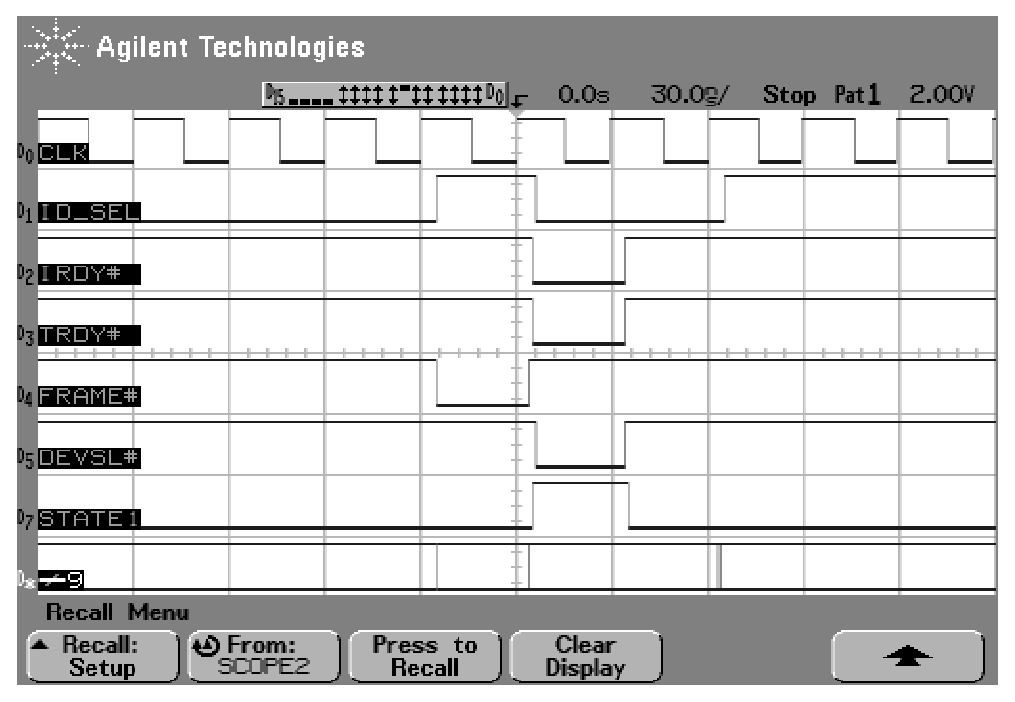
\includegraphics[width=\linewidth]{images/cfg_space_cap.eps}
\end{center}
\caption[PCI configuration space write transaction]{Screen capture of a PCI
configuration space write transaction.}
\label{PCI_CFG_Cap}
\end{figure}


\section{VGA and DVI Controller}
\label{VIDEO}

\mmodule{Patrick Suggate}{wb\_video\_top}
{This logic core reads 16-bit pixel data from the framebuffer and converts it to
24-bit colour, outputing this to the video DAC and TMDS encoder, as well as
generating all of the other signals necessary for redrawing the display.}
{/rtl/video/wb\_video\_top.v, /rtl/video/wb\_vga\_ctrl.v,
/rtl/video/wb\_redraw.v, /rtl/video/wb\_crtc.v, /rtl/video/crtc.v,
/rtl/video/vga16.v, /rtl/lib/fifo/afifo2k.v, /rtl/video/dvi\_ctrl.v}
{/sim/video/vga\_tb.v, /sim/video/crtc\_tb.v, /sim/xilinx/DCM.v,
/sim/xilinx/BUFGMUX.v}{GPL}

OpenVGA outputs image data, made up of multiple picture elements (called
``pixels''), to a standard computer display, typically a VGA connected CRT
monitor or a VGA or DVI connected LCD monitor. The VGA standard is analogue, so a
video DAC is used, the Philips TDA8777 IC -- since the Spartan-3 has no analogue
output pins, and DVI is a serial digital interface -- encoded using a TMDS
transmitter IC, via the Texas Instruments TFP410.

VGA and DVI display formats are 2D (2-Dimensional) and multicolour, and both the
VGA and DVI use similar control and synchronisation pulses\footnote{This was
intentional to accelerate the adoption of the newer DVI
specification\cite{VESA_DVI}.}. The display data, in graphical modes, is laid out
in memory as a flattened 2D array of pixel colours. To draw a complete screen of
data, this pixel colour information is sent, one pixel at a time, to the display,
using either a VGA or DVI connection. Display update rate is typically 60~Hz,
meaning that the display is completely redrawn 60 times per second.

The block of memory that stores the pixels for a 2D display is called a
frame-buffer. The size of this memory depends on the screen resolution and the
colour depth (and can be from 1-bit to 32-bits per pixel).

\begin{figure}[h!]
\begin{center}
\includegraphics[width=\linewidth]{images/video_controller.eps}
\end{center}
\caption[Video controller block diagram]{Video controller block diagram.}
\label{VIDEO_Ctrl}
\end{figure}


\subsection{Display Modes}

\subsubsection{Text Mode}
The original IBM VGA had hardware accelerated text modes that converted ASCII
characters, and an additional attribute byte, into pixel data as the screen was
being redrawn. This allowed a very small block of memory to represent the pixels
of an entire screen of text data. Additionally, the ASCII to pixel conversion is
quite slow on a general purpose CPU, and would have been prohibitively so in
1981~\cite{VGA_Programmers}, which is why the original IBM Monochrome Display
Adapter (MDA), and subsequent display adapters, used dedicated logic for the
task.

OpenVGA does not use legacy dedicated hardware for this ASCII to pixel conversion
as the on-board processor is capable of performing this task\footnote{The
original IBM XT ran at only 4.77 MHz, and required multiple clock cycles to
execute a single instruction, and had quite a slow system bus\cite{SVGA_Book}.
TTA16 can operate at up to 190 MHz, executes an ALU operation every clock cycle,
and has a fast connection to the framebuffer.} OpenVGA's firmware will contain
the code necessary for the ASCII to pixel transformation.
Appendix~\ref{Source_Code} contains the text-mode routines written in C. Assembly
for both RISC16 and TTA16 was written, based upon the C code, and used to
evaluate each processor.

\begin{figure}[h!]
\begin{center}
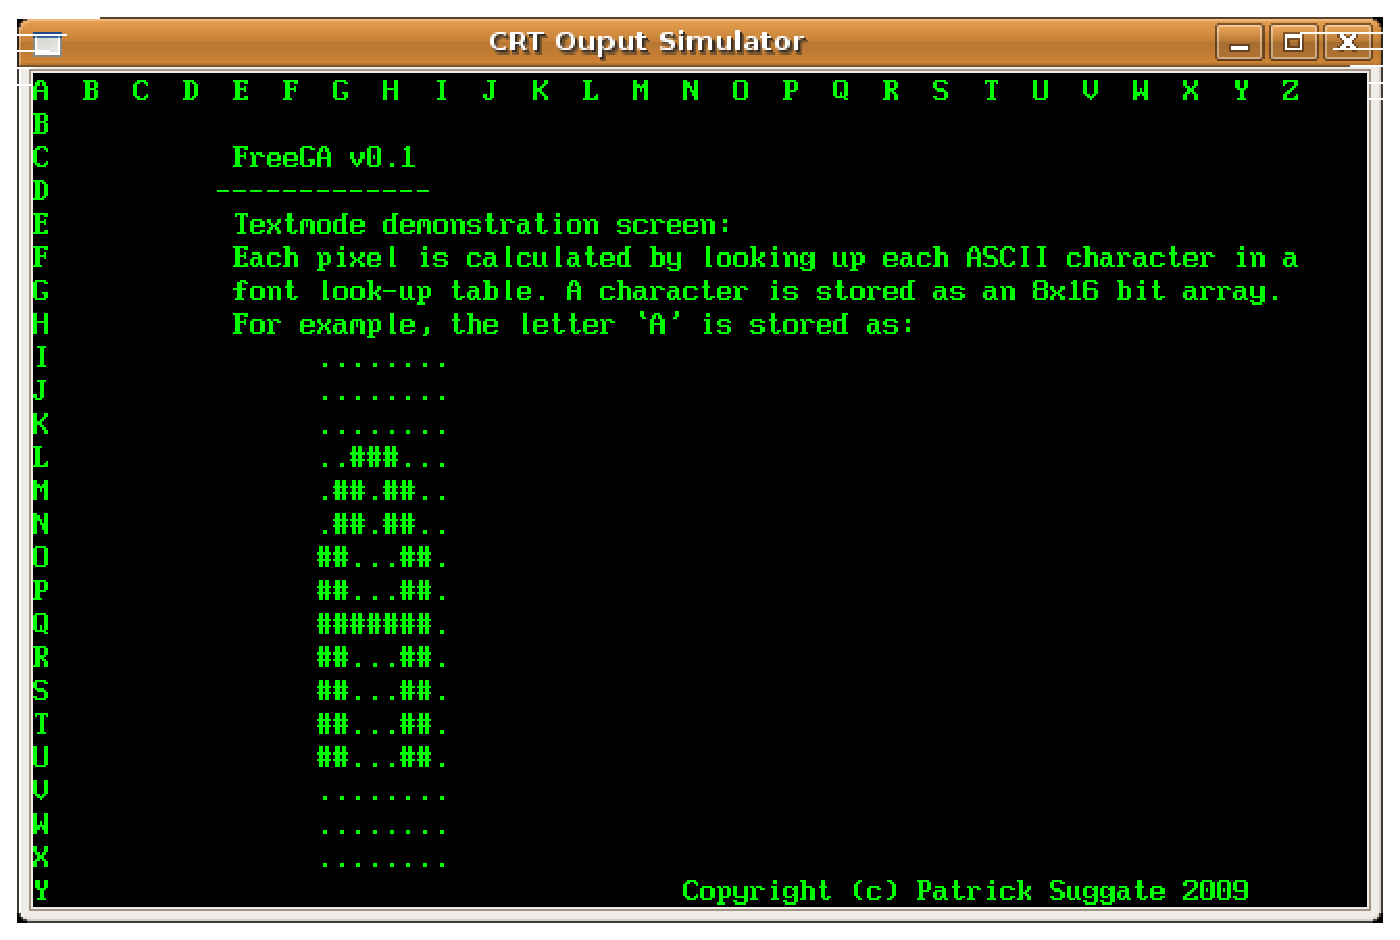
\includegraphics[width=\linewidth]{images/crt_sim.eps}
\caption[Emulated text-mode display data produced by a simulation]{Emulated
text-mode display data produced by a simulation.}
\label{CRT_Sim}
\end{center}
\end{figure}

To display the output of simulations of text mode, a Python script was written
that takes in the generated pixel data and displays it in a window. The results
produced by both the Icarus Verilog test-harnesses and the C code can then be
verified. A screen capture of the generated text-mode output is shown in
Figure~\ref{CRT_Sim}.

\subsubsection{Graphic Modes}
\label{VIDEO_Modes}
The current version of OpenVGA has only two frequencies available as the clock
source for the display timing, 25 MHz and 40 MHz. Table~\ref{VIDEO_Modes_Table}
shows common modes which use these dot clock frequencies.


\begin{table}[h!]
\begin{center}
\begin{tabular}{l r r r l}
				& 640x400	& 640x480	& 800x600	& Unit	\\
				& (VGA text)& (VGA)		& (SVGA)	&		\\
\hline
\textit{General Timings}	&	&	&	& \\
Dot Clock		&	25		&	25		&	40		& MHz	\\
H-sync			&	31.5	&	31.5	&	37.9	& kHz	\\
V-sync			&	70		&	60		&	60		& Hz	\\
Redraw data rate&	36.9	&	34.6	&	57.6	& MB/s	\\
\textit{Horizontal Timings}	&	&	&	& \\
Front porch		&	16		&	16		&	40		& clock cycles	\\
Back porch		&	48		&	48		&	88		& clock cycles	\\
H-sync duration	&	96		&	96		&	128		& clock cycles	\\
H-total			&	800		&	800		&	1056	& clock cycles	\\
\textit{Vertical Timings}	&	&	&	& \\
Front porch		&	12		&	10		&	1		& clock cycles	\\
Back porch		&	35		&	33		&	23		& clock cycles	\\
V-sync period	&	2		&	2		&	4		& clock cycles	\\
V-total			&	449		&	525		&	628		& clock cycles	\\
\end{tabular}
\end{center}
\caption[OpenVGA video modes]{OpenVGA video modes which use a dot-clock of
either 25 MHz or 40 MHz.}
\label{VIDEO_Modes_Table}
\end{table}

\subsection{Pixel Data Prefetch}
\label{VID_Prefetch}

The OpenVGA display data is stored in the SDRAM, which is in the Wishbone clock
domain, and needs to be prefetched and queued within the dot-clock domain for
redrawing the display. The data needs to be prefetched since the SDRAM is shared
with other peripherals but a steady stream of data is needed to redraw the
display without artifacts\footnote{The required data rate to redraw the display,
at a resolution of 640x480, and 16-bit colour, is 50 MB/s. Pixel data has to be
ready at each edge of the dot-clock when redrawing or else that pixel is
skipped.}

A 2 kB asynchronous FIFO achieves both these requirements, synchronises data
which has to cross clock domains, and queues up a large quantity of pixel data so
redraw can occur uninterrupted. The FIFO's half-full signal is used to trigger
prefetches, which are always 256 byte burst read transfers from the SDRAM
controller, as this is the SDRAM column size with the 8 MB SDRAM that was used.


\subsubsection{Video Clocks}
The signals to drive a display device, like a monitor, exist in their own clock
domain as well. This is because different video modes typically use different
pixel clocks to fetch and display pixel data, therefore has to be decoupled from
the system's internal bus clock. For example, the display mode 640x480 @60 Hz
uses a 25.175 MHz clock, 800x600 @60 Hz uses a 40 MHz clock, and 1024x768 @60 Hz uses
a 65 MHz clock. To transfer data from the clock domain of the system's Wishbone
bus to the video redraw circuit's clock domain, another asynchronous FIFO is
needed, but only one since data is transferred in just one direction. This
asynchronous FIFO was implemented using a BRAM and also functions as a prefetch
queue (see Section~\ref{VID_Prefetch}).


\subsection{CRT Controller}
\label{VID_CRTC}

The CRT Controller (Cathode Ray Tube Controller, called this for historic
reasons) generates the horizontal and vertical refresh signals which determine
the display resolution. To redraw the display, pixels are drawn from the top
left to the bottom right of the display\cite{VGA_Programmers} (see
Figure~\ref{INTRO_CRT_Redraw}). The display is redrawn row-by-row with a
horizontal synchronisation pulse marking the end of every row. Once all rows have
been redrawn, a vertical synchronisation pulse marks the end of the screenful of
data.

The basic design of the CRTC is two counters, a column counter and a row counter.
The column counter increments at each positive edge of the dot-clock until the
column limit is reached and then restarts at zero. Every time the column counter
resets to zero, the row counter increments until it reaches its row limit, and
then resets to zero.


\subsection{VGA Output}
\label{VIDEO_VGA_Output}

OpenVGA's output to a VGA monitor are three analogue colour components (red,
green, and blue), the horizontal synchronisation signal (subsequently referred to
as hsync), and the vertical synchronisation signal (subsequently referred to as
vsync).

The analogue signals are generated by an external video DAC since the Spartan-3
has no analogue outputs. The video DAC is connected to the Spartan-3 in 24-bit
colour mode, and since OpenVGA's framebuffer is stored as 16-bit colour data, to
reduce memory bandwidth, this data has its Least Significant
Bits\glossary{name={LSB}, description={Least Significant Bit}} (LSBs) padded with
zeros.


\subsection{DVI Output}
\label{VIDEO_DVI_Output}

The DVI transmitter IC is connected to the Spartan-3 in 12-bit DDR mode, which
means half the 24-bit colour is transferred on each clock edge. DVI support is
incomplete and the DVI output functionality has been only partially simulated but
not tested on OpenVGA hardware due to time constraints.


\section{Miscellaneous Peripherals}

\subsection{LEDs}
\label{LED_Driver}

\mmodule{Patrick Suggate}{wb\_leds}
{MMIO module for driving on-board LEDs.} {/rtl/lib/wb\_leds.v}
{/sim/lib/wb\_leds\_tb.v}{GPL}

OpenVGA has two LEDs for diagnostic and debugging output. These are memory-mapped
to the address 0x480000 . The following listing is a TTA16 assembly routine from
the OpenVGA firmware that sets the LEDs.

\begin{center}
\begin{minipage}{0.8\linewidth}
\footnotesize
\verbatiminput{source/tta16_set_leds.tex}
\normalsize
\end{minipage}
\end{center}

% \begin{lstlisting}[language={[x86masm]Assembler}]
% ; set_leds - The two LSBs of `r0' determines the LED outputs.
% set_leds:	{		,		,		,1	}
% 		{		,		,com	->msr	,0x48	}
% 		{\r0	->wad	,		,\r0	->mem	,1	}
% 		{\r15	->bra	,		,com	->msr	,\r12	} ; Restore SS
% 		{		,		,		,	}
% \end{lstlisting}


\subsection{USB Serial Port}
\label{USB_Sport}

\mmodule{Jeung Joon Lee, Patrick Suggate}{wb\_serial\_port}
{A Wishbone interface to a standard UART.} {/rtl/lib/wb\_serial\_port.v,
/rtl/lib/uart/*} {/sim/lib/wb\_serial\_port\_tb.v}{Modified BSD, GPL}

A USB port was also included as part of the OpenVGA hardware. This is connected
to the FPGA via a FTDI serial port IC. The Wishbone module allows the CPU to send
and receive data via the serial port, with the goal of being able to dump
OpenVGA's state, to aid with debugging OpenVGA.

The UART modules used as part of \texttt{wb\_serial\_port} is an open source
module, with a very permissive license, and was obtained from OpenCores.org, a
repository of open source HDL modules. The baud rate is configurable in the
Verilog code and currently operates at 9600 baud, 8-bits data, one stop-bit, and
no parity-bit.


% Errata, progress
\chapter{Summary, Conclusions, and Future Work}
\label{CONCLUSION}

Concluding this thesis is a summary of OpenVGA, the useful logic cores that were
developed, how these cores compared to those of other projects, and possibilities
for future work following on from this project. Future work, even if completed by
others, can be directly contributed back to the OpenVGA project. This is because
OpenVGA is an open-source project and licensed under the GPL.


\section{Summary of the OpenVGA Project}

OpenVGA development has reached the point where it can function as a secondary
graphics adapter. The OpenVGA local memory, an 8 MB SDRAM IC, is mapped into the
host system's address space, and its contents are accessible via the PCI Local
Bus. The contents of a portion of this memory, the framebuffer, can be displayed
on a VGA monitor, either a CRT or LCD display, that is connected to OpenVGA.

The design of OpenVGA is also very modular, and many of its components
interconnect using standard protocols. This applies to both the connections to
and from the PCB, connections between components on the PCB, and connections
between the logic cores within the Spartan-3 FPGA.

OpenVGA also contains a processor, implemented within the FPGA, with associated
firmware for initialisation tasks. Additional functionality can easily be added
by writing additional firmware. Firmware can be included during synthesis, stored
in the on-board serial PROM, or uploaded through the PCI Local Bus. OpenVGA was
designed so that this on-board processor can be used to emulate a subset of VGA
functionality. This would allow it to function as a primary graphics adapter once
complete, but this is future work.

A Linux kernel module has been developed that allows software to access OpenVGA's
local memory. Data can be written to, and read from, OpenVGA using this kernel
module. Any data written to the framebuffer region of memory will be displayed on
a VGA monitor connected to OpenVGA.

Software has been produced for this project too. There are utilities for
converting data between the different formats required, such as the tool to
convert the files generated by the assembler into a format that can be included
within the processor's Verilog source code. Other tools developed are an
assembler for RISC16, a CRT simulator for developing the display-controller logic
core, and a cache simulator that was used to analyse and select cache design
parameters, and code to simulate text-mode.

The text-mode simulator was written to provide a realistic workload for the
processor when choosing cache parameters. This piece of code would be a good
starting point for developing firmware to support VGA's alphanumeric
display-modes.


\section{OpenVGA Logic Cores}
The complete set of OpenVGA digital logic circuits requires only a small quantity
of logic and it can be embedded into larger SoC projects with little penalty. The
complete design uses less than 1100 slices of the Spartan-3 FPGA that it was
synthesised for. The Spartan-3 used does not contain a lot of programmable logic
compared to many other FPGAs, it is the second smallest device within the
Spartan-3 product range~\cite{Xilinx_SP3_DS}. OpenVGA used only 60\% of the
available FPGA logic. According to Xilinx, the XC3S200 is supposed to contain the
equivalent of about 200,000 logic gates, and modern ASICs can contain hundreds of
millions of logic gates.


\subsection{Summary of Important OpenVGA Logic Cores}
Many of the logic cores that have been developed for OpenVGA have been heavily
tested and optimised. All of the logic cores are written in the industry standard
Verilog HDL. Except for the asynchronous FIFOs, the external interfaces of these
logic cores are compatible with the Wishbone interconnect standard. These factors
mean that many of the following logic cores will likely be of use to other
projects.

The logic cores presented in Table~\ref{SUMMARY_Cores} are the sizes and speeds
of the cores when synthesised alone, with high optimisation settings, optimised
for speed, not area, and with parameters set to the configuration used within
OpenVGA. Theses numbers are approximate and depend a lot on many other factors.
Speeds will be lower when included in large designs, unless manually
floor-planned. And changing the optimiser setting to area, not speed, should
result in lower resource usage in more resource-limited designs.

\begin{table}[h!]
\begin{center}
\begin{tabular}{l | c c l}
Logic Core				& Speed	& Size	& Other logic elements used	\\
						& (MHz)	& (LEs)	&	\\
\hline
TTA16					& 190	& 200	& 2 BRAMs, 1 multiplier	\\
RISC16					& 140	& 320	& 1 BRAM, 1 multiplier	\\
Data Cache				& 150	& 80	& 1 BRAM	\\
PCI to Wishbone Bridge	& 110	& 320	&	\\
SDRAM Controller		& 120	& 100	&	\\
Display Controller		& 140	& 200	&	\\
Async. FIFO, 32-bit, 16-entry	& \texttt{>}150	& 60	&	\\
\end{tabular}
\caption[Summary of significant OpenVGA logic cores]{Summary of significant
OpenVGA logic cores.}
\label{SUMMARY_Cores}
\end{center}
\end{table}


\subsubsection{TTA16: A 16-bit TTA Processor}
A TTA processor logic core with a 32-bit instruction width, 16-bit data width,
4~kB of local instruction SRAM, three pipeline stages, and four data transports
was developed for OpenVGA. When synthesised for the Spartan-3, operating
frequency was up to 150~MHz, and using about 200 logic slices.

Unusual amongst processors, TTA16 does not support exceptions due to the extra
complexity this would have added to the design. This processor also features
interleaved instructions and no data-hazard interlocks, so it is difficult to
write assembly code for (see the programming guide in
Appendix~\ref{TTA_Programming}). The result is a processor that compares
favourably with other FPGA-based processors (see Table~\ref{SUMMARY_CPU_Table}).


\subsubsection{RISC16: A 16-bit RISC Processor}
This is a RISC processor with a 16-bit instruction width, 16-bit data width, 2 kB
of local instruction SRAM, five pipeline stages, and data forwarding. It was
developed for OpenVGA because TTA16 was such a difficult processor to write code
for and the result is a processor that is far easier to program (a programming
guide for RISC16 has been included as Appendix~\ref{RISCPROG}). Consequently, it
shares many of the same functional units and design techniques as TTA16, and
therefore has value for comparison with TTA16.

This logic core has the same external interfaces as TTA16 and these logic cores
be used interchangeably within a design, as long as the correct code is provided
for each processor as the instruction sets differ. Compared to TTA16, RISC16
operates at a lower frequency \texttt{>}100 MHz, but not higher than 140 MHz, and
uses more logic slices, 320 compared to 200, than TTA16, but is easier to
program. Creating a compiler would be easier as well, though beyond the scope of
this work.


\subsubsection{Data Cache}
The data cache can operate at more than 150 MHz and uses about 80 logic slices
when synthesised for a Spartan-3 FPGA (see Table~\ref{SUMMARY_Cores}). The data
cache significantly improved average memory latency with the text-mode conversion
algorithm, from 47 down to 5 clock cycles. This cache is 2 kB in size, a line
size of 64 bytes, and is a 2-way set-associative design. The cache sense logic
features a fast-hit path, with a latency of zero clock cycles, which is used when
calculating a hit within the same cache-line as the previous request. And a
slower-hit path, with a latency of one cycle, if the request is for a different
cache line.

An additional feature is that this cache is a dual synchronous-clock design. It
has two Wishbone interfaces, one that is connected to a processor and supports a
data width of 16-bits. The other Wishbone interface is to be connected to the
memory bus, which has a data width of 32-bits. The processor's Wishbone interface
can be driven at a frequency which is an integer multiple of the memory bus clock
frequency, as long as the two clock signals are synchronous, and both satisfy
their required timing constraints.


\subsubsection{Parameterisable SDRAM Memory Controller}
This memory controller design is simple, fast, and supports burst data transfers.
The maximum frequency at which the controller could operate, error free, was 120
MHz, which is 240 MB/s with a memory IC that has a 16-bit data bus, on a two
layer PCB with a Spartan-3.

The bit widths of the address, internal, and external data buses are
parameterisable. This memory controller can therefore be configured for many
applications. The configuration used within OpenVGA was a 32-bit internal data
bus width, an external 16-bit data bus width, and a 21-bit address width (the
size and speed for this configuration are shown in Table~\ref{SUMMARY_Cores}).

As an example, the controller could be parameterised to support an external bus
of 32-bits. This could be a design which used two 16-bit SDRAMs, or four 8-bit
SDRAMs. An external data width of 32-bits would require that the internal
Wishbone interconnect be 64-bits wide, since the external data bus operates at
twice the frequency of the internal bus.


\subsubsection{PCI-to-Wishbone Bridge}
The PCI-to-Wishbone bridge allows data to be transferred between clock domains
and bus protocols. The PCI Local Bus is a standard for transferring data between
components on system boards within a PC. The Wishbone interconnect is intended
for data transfer between logic cores within a single IC. This bridge features
asynchronous FIFOs so that PCI and Wishbone can operate within separate clock
domains. A FIFO is needed for each data-transfer direction, so two were used.

Even though the original PCI Local Bus specification is now considered obsolete,
and succeeded by PCI Express~\cite{budruk2003pes}, PCI is still popular and has a
considerable installed base. The PCI Local Bus is still found in many computers,
even those currently being produced. Due to the size of the installed base, there
are still reasons to use it, and therefore this logic core, in new designs.


\subsubsection{Video Controller}
This is a logic core that generates a data stream and the timing signals for
driving VGA and DVI monitors (though DVI is untested and this is future work).
This Wishbone-compatible core is sufficiently general-purpose and flexible to be
useful for any application which connects to a VGA or DVI display. The core
features a 2 kB prefetch queue, implemented using an asynchronous FIFO, so the
dot-clock and Wishbone clock can be in separate clock domains. The data prefetch
also makes the display redraw less susceptible to memory bus congestion.


\subsubsection{Asynchronous FIFOs}
Two asynchronous FIFOs were developed, one with 16 entries, and the other with a
capacity of 2048 bytes. These FIFOs are optimised for the Spartan-3 architecture,
to take advantage the of the Spartan-3 RAM primitives for efficient
implementation. The width of the data bus is parameterisable for the 16-entry
FIFO. A width of 32-bits is used for the PCI-to-Wishbone bridge, and
Table~\ref{SUMMARY_Cores} lists the speed and size in this configuration.

Asynchronous FIFOs are important when multiple bit-width data needs to be
transferred across clock domains. The design of these FIFOs ensures that
metastability problems are avoided~\cite{Async_FIFO2}.


\subsection{Processor Comparison and Summary}
\label{SUMMARY_CPU}
Two processors were developed for OpenVGA, a traditional RISC design, RISC16,
and a processor with a novel transport-triggered architecture, TTA16 . Relative
to RISC16, the TTA16 processor uses fewer logic resources, operates at higher clock
frequencies, and can perform more operations per clock cycle (see
Section~\ref{TTA16}).

RISC16 has a 16-bit instruction word, instead of the 32-bit wide instructions of
TTA16, leading to far better code density. It is also a simpler architecture to
program in assembly language, data-forwarding and interlocking help here, and
RISC16 is similar to processors with GCC ports. But due to the added complexity
of RISC16 it is both larger and slower than TTA16 .


\begin{table}[h!]
\begin{center}
\begin{tabular}{l | r r c c l}
CPU Name & Speed & \multicolumn{1}{c}{Size} & Compiler & Open- &
Notes \\

	& \multicolumn{1}{c}{(MHz)}	& \multicolumn{1}{c}{(Slices)} & & Source & \\
\hline

MicroBlaze~\cite{xilinx2008mpr} & 115 & \~1000 & Yes & No & Proprietary \\

PicoBlaze~\cite{xilinx2008ppr} & 90 & 90 & No & Yes & Limited address space \\

ZPU~\cite{ZPU} & 90 & \~400 & GCC & Yes &	\\

OR1k~\cite{OpenRISC} & 30 & 2000 & GCC & Yes &	\\

GR0040~\cite{FPGACPU} & 30 & 200 & LCC & Yes & Restrictive license \\

RISC16 & 140 & 320 & No & Yes & Lcc port possible	\\

TTA16 & 190 & 200 & No & Yes & \begin{minipage}{0.3\linewidth} Fast but
difficult to program and poor code density. \end{minipage} \\

\end{tabular}
\caption[Evalualted processors and a comparison with TTA16 and
RISC16]{Evaluated processors and a comparison with TTA16 and RISC16.}
\label{SUMMARY_CPU_Table}
\end{center}
\end{table}

A summary of the processors that were compared with TTA16 and RISC16 are listed
in Table~\ref{SUMMARY_CPU_Table}. All of the operating speeds and numbers of
logic slices used are approximate and depend heavily on the parameters used,
optimisation settings, and the other components within a design. This table just
indicates what can be expected in best-case scenarios.

In terms of size and performance, both of OpenVGA's processor logic cores compare
favourably to other FPGA-based processors, as Table~\ref{SUMMARY_CPU_Table}
shows. TTA16 is the standout here in terms of performance, and RISC16 is fast as
well. All processors listed have assemblers, but TTA16 and RISC16 lack C
compilers. ZPU, MicroBlaze, and OR1k are all 32-bit processors, so based on this
table, ZPU is clearly the best of these. It would have been a good candidate for
OpenVGA, but unfortunately this processor only recently reached a usable
state~\cite{ZPU}.


\subsection{Known Bugs}
There exists a known bug within the SDRAM controller logic core and this is
covered in Section~\ref{SDRAM_Bug}. Fortunately, this is the only known bug with
OpenVGA, and there is a software workaround. The size of burst transfers can be
limited, which seems to solve the problem. Fixing this bug is future work.


\section{Future Work}
Open-source hardware is an area which is still in an early state of development.
There is no free and open implementation of a VGA-compatible graphics adapter. An
obvious direction for OpenVGA to take is enough VGA support to allow it to
function as a PC's primary graphics adapter. OpenVGA was designed as a step
towards VGA functionality and features a processor suitable for this task.

Another avenue of future work discussed here is software drivers so that OpenVGA
can be used with the Graphical User Interfaces (GUIs) of modern operating
systems, like GNU/Linux, Windows, and Mac OSX. Other areas for future work
include improvements to the hardware, like PCI Express support, using a more
modern FPGA, and greater memory bandwidth. These changes will require changes and
additions to the current set of logic cores as well.


\subsection{VGA Compatibility}
OpenVGA does not currently a VGA-compatible graphics adapter, this is due to the
lack of the firmware for VGA emulation. Chapter~\ref{BACKGROUND} covers the
components of a VGA which will have to be emulated. The quantity of firmware code
required is substantial and was beyond the scope of this project. A C compiler
would simplify this task, and could be another area of research.


\subsection{Software}
Due to PCI Plug and Play support, OpenVGA is detected and initialised correctly
by the host system, but it is not currently taken advantage of by any operating
systems since only a simple Linux kernel module has been written, and just for
testing purposes. A driver for X11 or Microsoft Windows would allow OpenVGA to be
a supported display device for these operating systems. Writing an X11 driver
should be straight-forward, since the OpenGraphics project has an open-source
driver available.

If OpenVGA is used for other uses, such as hardware computation, it will most
likely require additional custom software and drivers, though the current kernel
module may be enough for some applications, since it allows OpenVGA to be written
to, and read from, like a file.

TTA processors that have multiple data-transports are very time consuming to
program in assembly code. TTA16 would be a far more useful processor if there
was a C compiler for it. There are open-source C compilers for other TTA
processors~\cite{jaaskelainen2007cta, corporaal1993maa}, these are GCC ports,
and maybe one of these could be modified for TTA16 . Generating optimised
code for TTA processors is very difficult though.


\subsection{Hardware Improvements}
% TODO: DVI testing.
OpenVGA hardware works well and is low-cost but future modifications could
significantly improve performance and features. By changing to a four-layer PCB,
adding a PCI-Express PHY, an on-board clock-generator IC, a larger FPGA with more
I/O pins, and larger, wider, and faster memory IC would allow OpenVGA to support
high-resolution video modes, and allow it to be more useful for hardware
computation tasks. A current area of research, for example, is real-time
ray-tracing\cite{wald2004rrt, TTA_Ray_Trace}.

Xilinx have recently introduced a new low-cost FPGA product line, the Spartan-6
family, replacing Spartan-3 generation FPGAs. These are faster and have more
logic resources than their previous generation devices. FPGAs from other vendors
should be evaluated as well, like the Cyclone III from Altera, or a Lattice
ECP3\footnote{A disadvantage with Altera and Lattice is that these vendors do not
have a free tool-chain that supports the GNU/Linux operating system, only
currently Microsoft Windows.}. Another benefit of these newer FPGAs is they have
hardware support for DDR2 and DDR3 memory, addressing a current OpenVGA weakness.


\subsection{Logic Core Improvements}
There are two options for improving the current logic cores. The first approach
would be changes that expand the functionality of OpenVGA, and the second class
of improvements would optimise the current set of logic cores.

\subsubsection{New Features}
To complete VGA-compatibility, the PCI-to-Wishbone bridge would need modifying
so that it identifies itself as a VGA device. This is straight-forward, and is
covered here~\cite{PCI_Spec}.

It is also common for graphics adapters to contain logic for hardware
acceleration of 2D and 3D tasks. Some support for this could be done through
firmware with the existing processors, new functional units could be added to
these processors\footnote{Automatic synthesis of TTA processors is a possibility
too~\cite{hoogerbrugge1995ast}, this would allow processors to be developed
quickly for specific uses.}, or new logic cores could be added that provide this
functionality.


\subsubsection{Optimisations}
While individual logic cores have been heavily optimised for speed and size, they
could be modified to make more efficient use of the buses which connect them
together. For example, the PCI-to-Wishbone bridge does not use the burst-transfer
functionality of the Wishbone interconnect standard, nor does it support PCI
burst read transfers. This is because the logic required to support this is quite
complex. These changes will lower bus congestion, thereby increasing system
performance.

Another area that can be optimised is the cache. Currently, when the processor
performs a memory write it stalls until the completion of the transaction, which
can be many cycles. A write-back cache design reduces the frequency of this
problem. Also, when a memory read is issued by the processor, and if there is a
cache miss, the processor stalls until the entire cache-line has been fetched. It
would be possible to implement a system where the desired word is fetched first,
and then allowing the processor to continue operation.

A change to the SDRAM controller, adding write-data FIFOs, would allow multiple
memory writes to be queued, and completed at a time suitable to the memory
controller. This modification would probably add 60 logic slices to the size of
the controller though.


\section{Conclusion}
The design and construction of a low-cost, open-source graphics adapter has been
presented in this thesis. Open-source hardware is a relatively new area of
research. As long as the capabilities and price of programmable logic keeps
improving, open-source hardware will likely be an expanding domain too. This
project contributes OpenVGA to this area. Both as a stand-alone project, and as a
collection of free and open logic cores.



\bibliographystyle{plain}
\bibliography{thesis_bib}

\appendix
\chapter{Source Code Layout and Overview}
\label{Source_Code}

OpenVGA is an open-source project, licensed under the GPL. All of the source
code is available on the Internet. The URL is http://openvga.sourceforge.net/
and also contains the snapshot of the project at the point of the completion of
this thesis.

\section{Top-Level}

Also included in the top-level are the standard LICENSE and README text files
which are included within most open-source projects.

\begin{flushleft}

\begin{tabular}{l l}

\textbf{rtl/} & \bigdescript{0.8}{Verilog RTL (Register Transfer Level)
description of the design. There is a Makefile to synthesise the design
using XST and targeting the Spartan-3 FPGA family.} \\
\\

\textbf{sim/} & \bigdescript{0.8}{Verilog RTL (Register Transfer Level)
description files for the test-harnesses of the logic-cores in this
project.}\\
\\

\textbf{src/} & \bigdescript{0.8}{OpenVGA source code for kernel driver, the TTA
assembler, the RISC16 assembler, the cache and text-mode
simulators, and a partial VGABIOS implementation.}	\\
\\

\textbf{tools/} & \bigdescript{0.8}{Scripting files used for tasks such as
assigning data to BRAMs, converting fonts, and a CRT simulator.} \\
\end{tabular}

\end{flushleft}



\section{HDL Hierarchy}

The Verilog source code is consists of both logic-core source files and hardware
testbenches. Simulation test-harness code is in a separate {\texttt sim}
directory.

\begin{flushleft}

\begin{tabular}{l l}
\textbf{rtl/} & \bigdescript{0.75}{The top-level OpenVGA modules, testbenches,
and makefile.}	\\
\\

\textbf{rtl/cpu/} & \bigdescript{0.75}{Both the RISC16 and TTA16 processors, and
hardware testbenches.}	\\
\\

\textbf{rtl/lib/} & \bigdescript{0.75}{Library containing copies of modules not
specific to the OpenVGA project. This includes LFSRs, multiplexors, FIFOs.}	\\
\\

\textbf{rtl/misc/} & \bigdescript{0.75}{Miscellaneous modules, and testbenches,
that are too OpenVGA specific for the ``lib'' directory.}	\\
\\

\textbf{rtl/pci/} & \bigdescript{0.75}{The files for the
PCI-to-Wishbone Bridge logic core and a hardware testbench.}	\\
\\

\textbf{rtl/sdram/} & \bigdescript{0.75}{SDRAM controller logic core modules and
hardware testbench.}	\\
\\

\textbf{rtl/video/} & \bigdescript{0.75}{The OpenVGA video logic core. There are
CRTC, prefetch buffer, redraw logic, and hardware testbench modules.} \\
\end{tabular}

\end{flushleft}



\section{Simulation Test-Harness Hierarchy}

This directory contains the Verilog simulation files for the logic cores within
the \texttt{sim} directory.

\begin{flushleft}

\begin{tabular}{l l}
\textbf{sim/} & \bigdescript{0.75}{The top-level OpenVGA, module
test-harnesses, and Makefile.} \\
\\

\textbf{sim/cpu/} & \bigdescript{0.75}{RISC16 and TTA16 simulation
test-harnesses for use with Verilog simulators.}\\
\\

\textbf{sim/lib/} & \bigdescript{0.75}{Library containing test-harnesses for
modules not specific to the OpenVGA project. This includes test-harnesses for
LFSRs, multiplexers, FIFOs. Additionally, many Xilinx built-in primitives were
emulated and these modules and test-harnesses are within this folder as well.}
\\
\\

\textbf{sim/misc/} & \bigdescript{0.75}{Miscellaneous test-harnesses for
modules that are too OpenVGA specific for the ``lib'' directory.} \\
\\

\textbf{sim/pci/} & \bigdescript{0.75}{Test-harnesses used while developing
the PCI logic core.}	\\
\\

\textbf{sim/sdram/} & \bigdescript{0.75}{SDRAM controller test-harnesses.}	\\
\\

\textbf{sim/video/} & \bigdescript{0.75}{The OpenVGA CRTC, prefetch buffer,
redraw logic, and testbenches.} \\
\end{tabular}

\end{flushleft}


\section{Tools}

There were many scripts and other tools created for this project. They are
typically used for converting data between the many formats used, like font data,
creating Verilog include files, and other post-processing tasks.

Other tools include \texttt{peek}, \texttt{poke}, \texttt{set}, \texttt{test},
and other OpenVGA test applications that were used for developing and testing the
PCI bridge and SDRAM controller. These were run on the host computer that OpenVGA
was attached to.



%============================================================================
\chapter{OpenVGA Components and PCB}
\label{HARDWARE}

This appendix provides more detail of the OpenVGA hardware. The CADSoft
Eagle\texttrademark~schematic, board, and parts-list files are available on the
Internet from http://openvga.sourceforge.net/. OpenVGA uses of a two-layer PCB
for cost and simplicity and the PCB form-factor is a full-height, short, PCI
expansion board with rear I/O panel connectors (see Figure~\ref{HARDWARE__PCB}).
Two-layer PCBs restrict the choice of electronic components due to routing and
signal integrity issues. Data-sheets of high-pinout BGA ICs often recommend
six-layer PCBs or more, for example~\cite{Xilinx_SP3_DS}.

\begin{figure}[h!]
\begin{center}
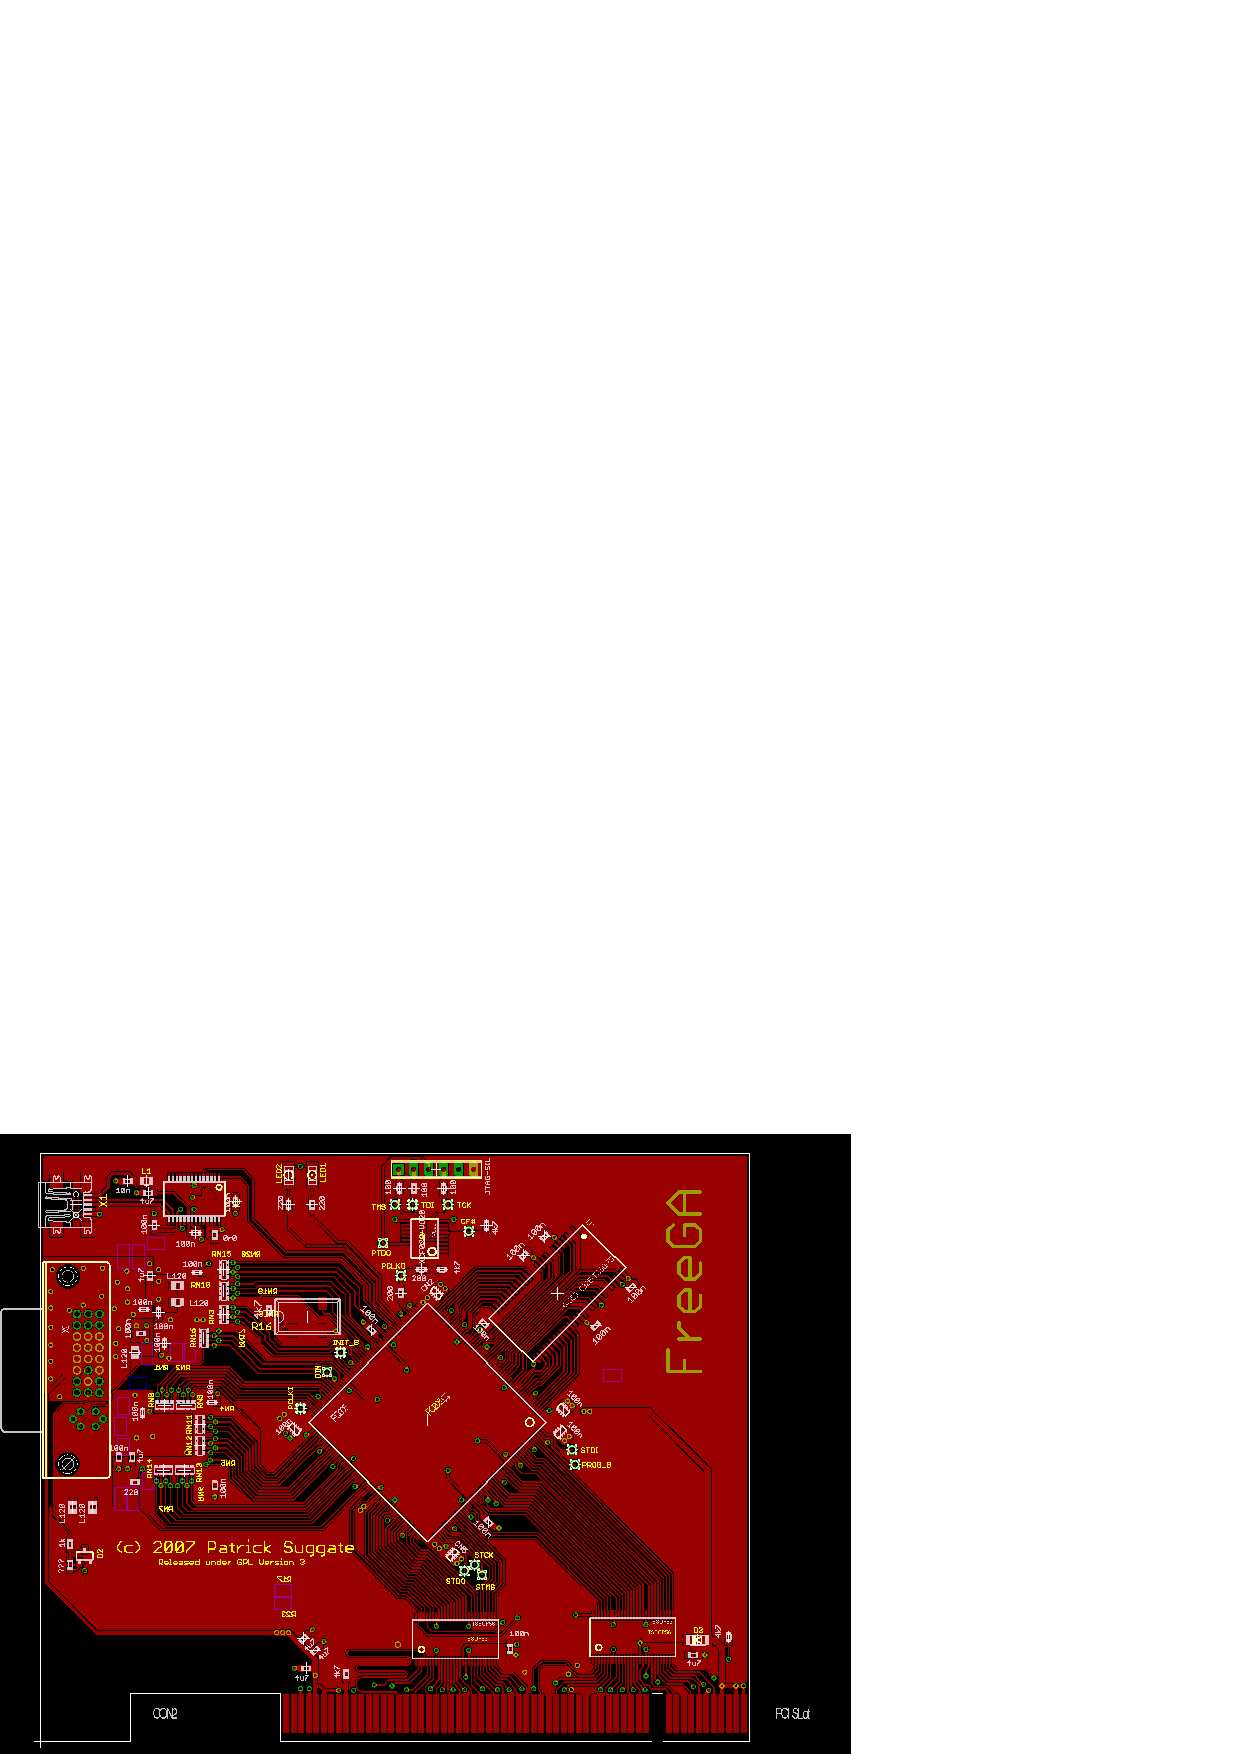
\includegraphics[width=0.49\linewidth]{images/freega3_pcb_art_top.pdf}
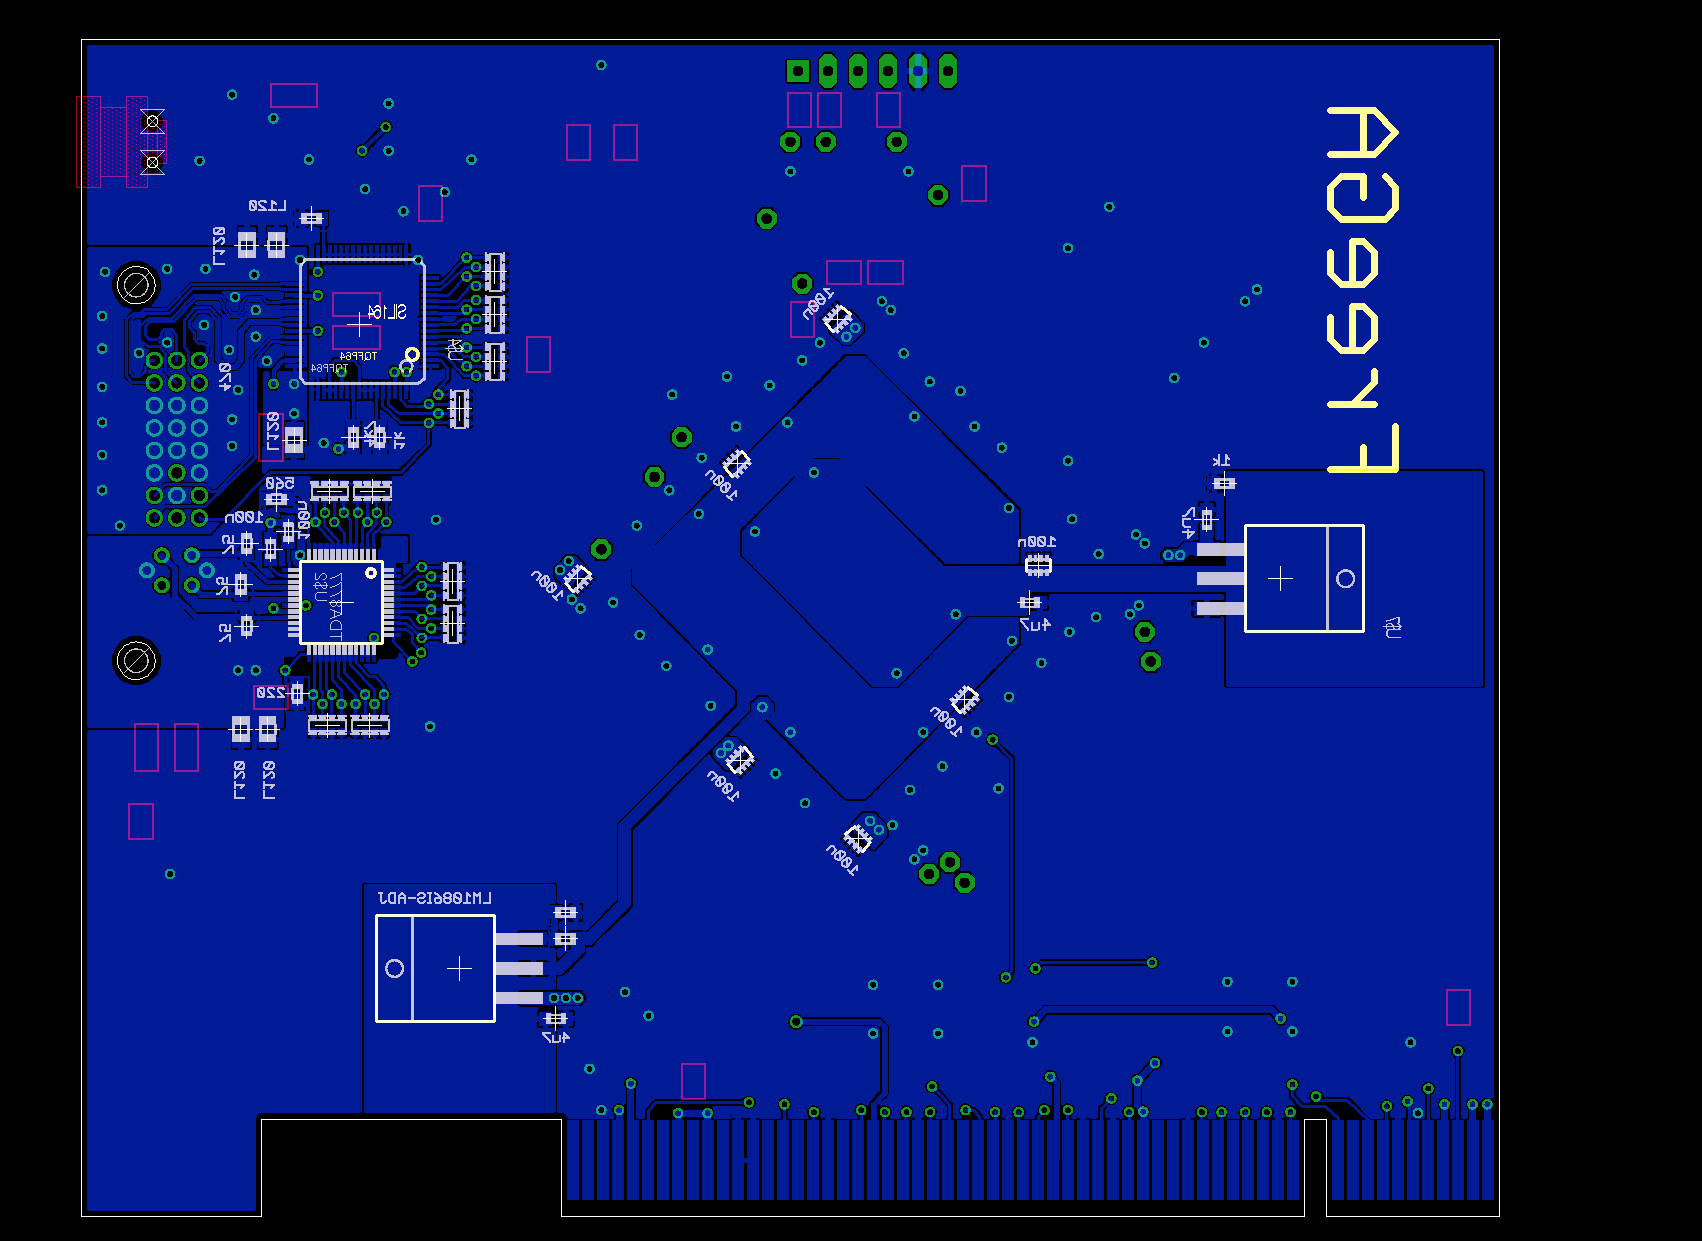
\includegraphics[width=0.49\linewidth]{images/freega3_pcb_art_bot.pdf}
\end{center}
\caption[OpenVGA PCB artwork, both sides]{OpenVGA PCB artwork, both sides.}
\label{HARDWARE__PCB}
\end{figure}


The FPGA has mostly user assignable inputs and outputs so this allowed flexible
placement of most of the other ICs. The video transmitters could be near the back
edge of the PCB and SDRAM could be placed so as to minimise trace lengths.

The components were laid out with the objective of having the majority of the
signal routing on the top-layer (the component-side) so that the bottom-layer
(the solder-side) could be used for routing the power-supply and ground nets. The
VGA and DVI transmitter ICs were mounted on the solder-side as well, and this was
to simplify routing. The decoupling capacitors and termination resistors were
mounted on both sides of the PCB since they were required to be as close as
possible to their related ICs.


\section{Off-Board Connections}
OpenVGA has connectors for PCI, DVI, VGA (through the DVI connector, using an
adapter), JTAG, and USB (see Figure~\ref{OPENVGA_OpenVGA}. Only the JTAG
connections are connected directly to the FPGA, the rest use encoder or
voltage-translation ICs and are detailed below.


\section{Integrated Circuits}
Table~\ref{HARD_ICs} is a list of the ICs chosen for OpenVGA. More complete
descriptions are included in later sections of this appendix.
Figure~\ref{OPENVGA_OpenVGA} shows the ICs which are on the top (component layer)
of the PCB, the two video encoders, the TMDS encoder and the video DAC are shown
in Figure~\ref{HARD_Bot}.

\begin{table}[h!]
\begin{tabular}{l | l}
Part\#				& Description	\\
\hline
XC3S200-4PQG208C	&	Xilinx Spartan-3 FPGA, 200k Gates	\\
MT48LC4M16A2TG-75	&	Micron 8 MB SDRAM	\\
TDA8777HL/14/C1,15	&	Philips video DAC, 10-bits/colour component	\\
TFP410PAP			&	Texas Instruments TMDS encoder		\\
LM1086IS-ADJ		&	National Semiconductor SMT, adjustable, voltage regulators	\\
CBT16211DDG			&	Fairchild Semiconductor 24 I/O, Bus Switches	\\
XCF04SVOG20C		&	Xilinx 4 Mb, Platform Flash, Serial PROM	\\
FT232RL				&	Future Technology Ddevices International USB UART	\\
SG-8002JA-MPT		&	Epson Toyocom Corporation 50 MHz, SMD oscillator	\\
\end{tabular}
\caption[OpenVGA integrated circuits]{OpenVGA integrated circuits.}
\label{HARD_ICs}
\end{table}


\subsection{The Xilinx Spartan-3 FPGA and SPROM}
The core of OpenVGA is a FPGA which contains the logic necessary for implementing
this display device. The FPGA is a 200 k-Gate, Xilinx Spartan-3, XC3S200 FPGA,
which is from the Xilinx low-cost product range. It has a quantity of
programmable logic that Xilinx considers as approximately equivalent to an IC
with about 200,000 gates.

The FPGA can be programmed using a JTAG\glossary{name={JTAG}, description={Joint
Test Action Group}} boundary-scan chain or on power-on using a Xilinx SPROM. The
state of the Spartan-3 is lost on power-off~\cite{Xilinx_SP3_DS} so a SPROM
(Serial Programmable Read-Only Memory) is used to restore the state at power-on.
The SPROM is programmed using the JTAG boundary-scan chain as well.

The Spartan-3 requires multiple supply voltages. This Spartan-3 core logic runs
at 1.2 V, the I/O banks at 3.3 V, and the FPGA configuration circuitry at 2.5 V.
This complicates the power-supply routing when using a two-layer PCB, but
decoupling capacitors were used in accordance to Xilinx specifications and no
problems were experienced, even though Xilinx recommends separate power-planes
for each supply.


\subsection{The DVI and VGA Video Encoders}
The DVI TMDS encoder and the VGA video DAC are used to convert the parallel,
digital video signals generated by the FPGA into the signals (analogue for VGA,
TMDS for DVI) used by an attached DVI or VGA computer monitor. The TMDS encoder
and video DAC operate at high frequencies for a two-layer board so termination
resistors are used to improve signal quality. An early development version of
OpenVGA (as shown in Figure~\ref{OPENVGA_Version2}) had significant signal
integrity issues. Neither the DDR SDRAM or the TMDS encoder operated correctly.
The signal waveforms, as displayed on an oscilloscope, had significant undershoot
and overshoot. The current OpenVGA board with the terminating resistors has very
good signal integrity for a two-layer board.

\begin{figure}[h!]
\begin{center}
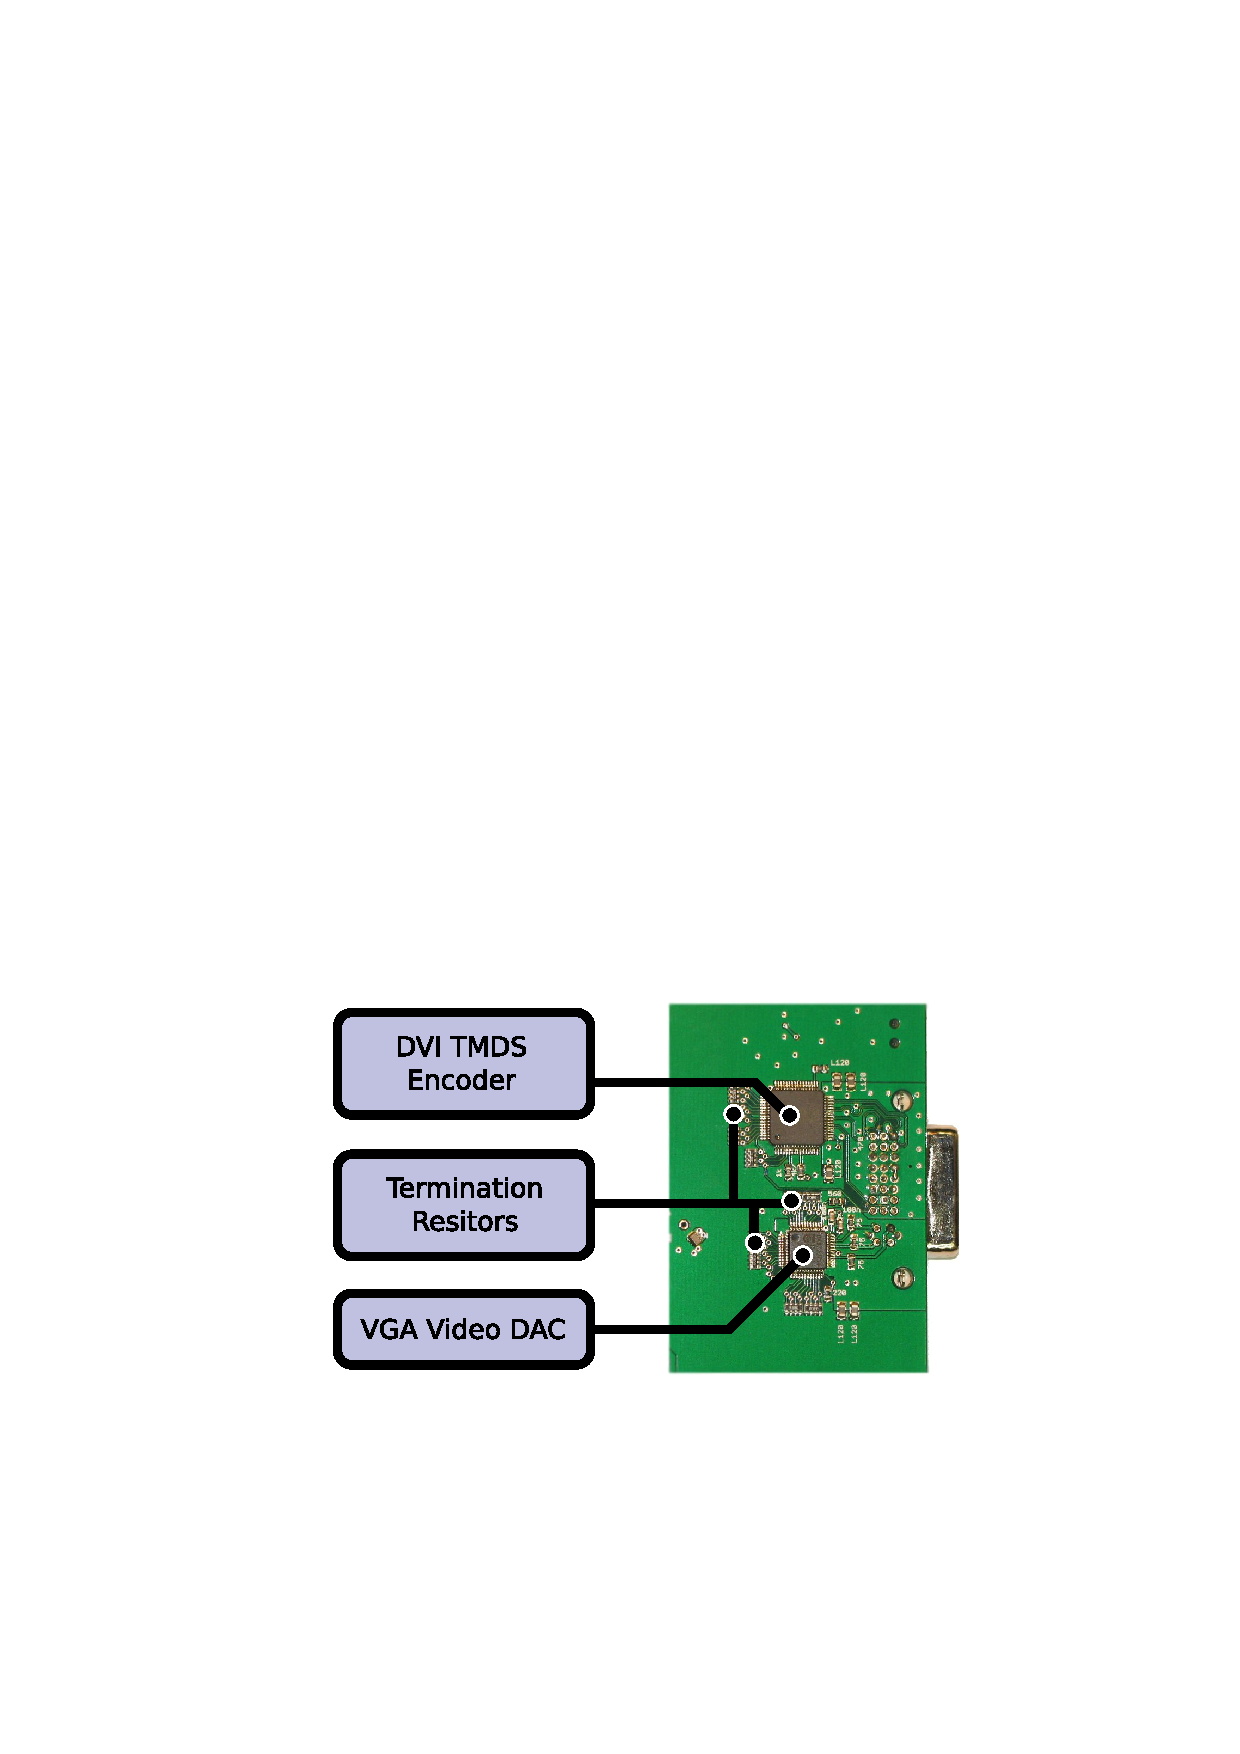
\includegraphics[width=0.5\linewidth]{images/openvga_bot.pdf}
\end{center}
\caption[OpenVGA solder-side components]{OpenVGA solder-side components.}
\label{HARD_Bot}
\end{figure}


\subsection{USB UART}
A logic core was developed which allows the OpenVGA processor to read to, and
write from, the USB UART. This can be used for debugging as well as interfacing
with the many devices which use this standard.


\subsection{PCI Bus Switches}
The PCI Local Bus uses half-wave reflection signalling~\cite{PCI_Spec, PCI_Book}
which causes voltage transients that exceed the maximum operating conditions
specified for the Spartan III family\cite{Xilinx_SP3_DS}. Two 24 pin bus switches
were used to prevent PCI signals from exceeding 3.4 V and -0.7 V. These switches
add a propagation delay of 250 ps~\cite{Bus_Switch_DS}.


\chapter{Wishbone Interconnect Overview}
\label{APP_Wishbone}

\section{Wishbone Interconnect Introduction}
Wishbone was designed as an internal interconnection standard for
System-on-a-Chip (Soc) applications (see www.OpenCores.org, the current home of
Wishbone project, and the contains the full specification). Wishbone is an
intended as a solution to provide a standard interface for communicating
between logic cores from multiple vendors. It can be difficult to
integrate logic cores if they each use a different interconnect scheme, and
this can also add significant overhead (logic and latency).

\subsection{Features}
The Wishbone design was inspired by traditional microcomputer
buses\cite{WB3_Spec}, like PCI and VME, as these are general purpose
interconnects that are flexible and robust.

A brief summary of important Wishbone features:
\begin{itemize}
  \item Supports reads and writes, burst and single-word transfers.
  \item Simple, logic resource requirements are low. At its simplest, an
  interface to a synchronous SRAM requires just one logic gate.
  \item User-defined tags allows the addition of extra signals.
  \item Support for data bit-widths of 8, 16, 32, and 64.
  \item Any address bit-width is supported, even zero, depending on the device.
  \item Synchronous; all transfers occur on clock edges.
  \item Choice of topology, i.e. bus, point-to-point, crossbar switch, is up to
  the system designer.
  \item Not encumbered by patents, free for all to use.
  \item A single device can be both a master and a slave.
  \item Offers some support for handling errors.
\end{itemize}


\subsection{A Simple Example}
In the timing diagram shown in Figure~\ref{APP_Wishbone_Sig}, the simultaneous
assertion of CYC and STB select the slave device, the WE signal indicates this
is a write transaction.

\begin{figure}[h!]
\begin{center}
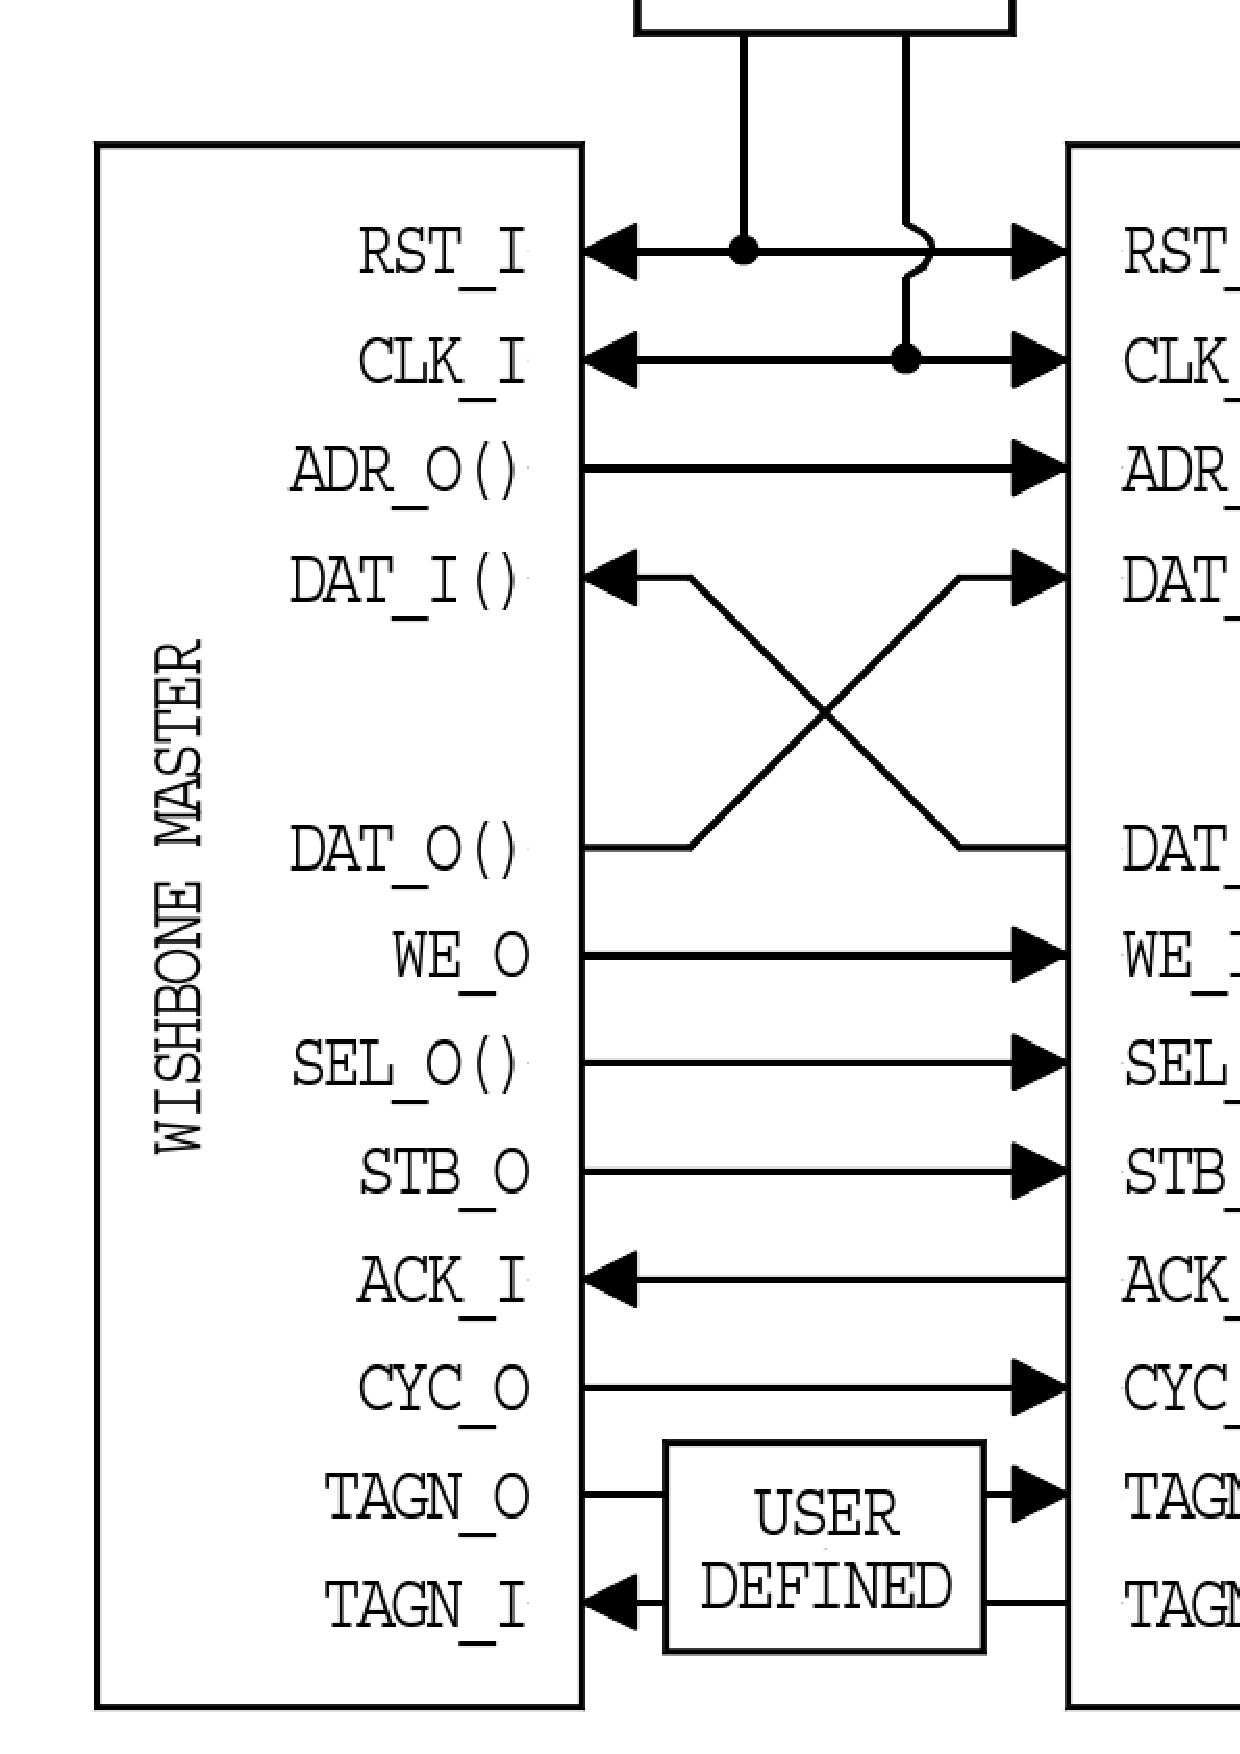
\includegraphics[width=8cm]{images/wishbone_bus.pdf}
% 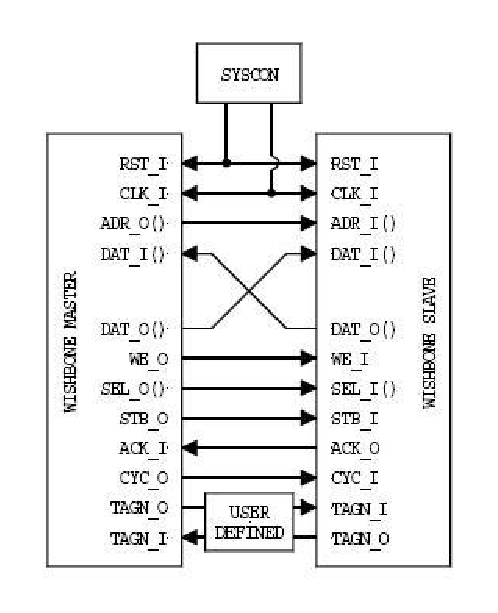
\includegraphics[width=8cm]{images/Wishbone_Bus_Point_to_Point.eps}
\caption[A Wishbone Point-to-Point Connection Scheme]{This is an example
implementation of a basic master-slave, point-to-point Wishbone interconnect.
The ``SYSCON'' design is not part of the Wishbone specification, it maybe
implemented however the designer sees fit.

Source: 'WISHBONE System-on-Chip (SoC)Interconnection Architecture for Portable
IP Cores', Revision: B.3, Released: September 7, 2002.}
\end{center}
\label{APP_Wishbone_P2P}
\end{figure}

\begin{figure}[h!]
\begin{center}
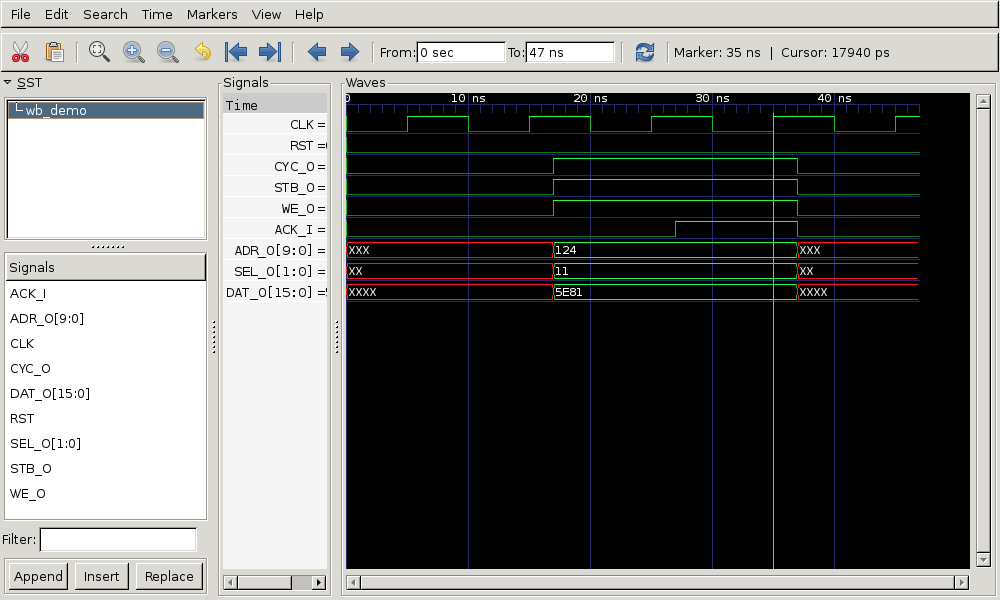
\includegraphics[width=\linewidth]{images/wishbone_demo.pdf}
\caption[A Sample Wishbone Transaction]{One 16-bit word is written by a master
to a slave device. The signals CYC$\_$O and STB$\_$O are asserted by the master to frame the transaction. The ACK$\_$I
response is received by the master and indicates that the slave has completed the
transfer.}
\end{center}
\label{APP_Wishbone_Sig}
\end{figure}


\section{Description of Wishbone Signals}
This section gives a brief summary of the main Wishbone signals. User-defined
tags were not used for OpenVGA's internal bus so these signals are not described.
Additionally, Wishbone bus ports to HDL modules used within OpenVGA include both
a prefix and a suffix. For example, the prefix ``wb'' of signal
``wb$\_$cyc$\_$o'' indicates that the signal is a Wishbone signal, and the
suffix ``o'' indicates that this is an output. (The output direction of the CYC signal would also
indicate that the module this signal belongs to is a Wishbone master.)

\begin{itemize}
  \item CYC: This signal is asserted by a master and it claims ownership of the
  Wishbone bus. Other masters on a bus are prevented from asserting their CYC
  when a CYC is already asserted. This signal is still used for non-bus
  topologies, like point-to-point, and is used in combination with STB to select a slave
  device.
  \item STB: This signal is asserted by a master and frames a Wishbone
  transaction. If a slave device has its STB input signal asserted, then it has
  been selected for a Wishbone transaction.
  \item WE: This signal is driven by a master and selects whether the
  requested transaction is a write or a read (signal levels high and low
  respectively).
  \item ACK: This signal is asserted by a slave to indicate that it has either
  received data, if the transaction is a write, or has placed valid byte
  selects and data on its data outputs, for a read transaction. This signal is
  asserted just once for each data transfer, and can take many cycles to assert, depending on the
  latency of the device.
  \item RTY: This signal is asserted by a slave to indicate that the device is
  currently unable to fulfil the current Wishbone request, and to retry
  later.
  \item ERR: This signal is asserted by a slave to indicate that an error has
  occurred. Wishbone does not specify how errors are handled except that the
  slave must leave the bus in a usable state at the end of the transaction.
  \item CTI[2:0]: This signal array is driven by the master and can request a
  burst transfer. Even if the master specifies a burst mode, the slave is not
  required to perform a burst transfer. Also, if the slave supports burst
  transfers but not the mode requested, it responds with single transfers. It
  is optional to implement this signal, it has to be set to zero for a slave
  that supports this signal when a master does not. A full description of the
  modes is available in the Wishbone specification\cite{WB3_Spec}.
 \item BTE[1:0]: This signal array is driven by the master and specifies the
 Burst Type Extension. This signal can only be implemented if CTI
 is also implemented, and is required to be implemented if CTI is implemented
 and the device supports burst transfers. A full description of the modes
 is available in the Wishbone specification\cite{WB3_Spec}.
 \item ADR: This signal array is driven by the master and is the
 address of the data requested for the transaction. This signal is
 optional, and its width is device dependent, a FIFO may not need an address,
 for example.
 \item SEL$\_$O[$n$-1:0] \& SEL$\_$I[$n$-1:0]: These signal arrays are driven
 by both masters and slaves and are used to select valid bytes within a data
 word. A 64-bit transfer has eight select bits, so $n=8$, for example. During a
 write transaction, the master asserts the valid bytes on its own SEL$\_$O
 outputs, and during a read transaction, the slave asserts the byte-valid
 selects on its SEL$\_$O outputs. A device that supports reads and writes is
 required to implement both SEL$\_$O and SEL$\_$I. These signals have to
 be valid when the device responsible for driving them has its STB or
 ACK signals asserted.
 \item DAT$\_$O[$m-1$:0] \& DAT$\_$[m-1:0]: These signal arrays are driven by
 both masters and slaves and are used to transfer data across the Wishbone
 interconnect. The width, $m$, must be one of 8, 16, 32, or 64. A master
 performing a write must have valid write data on its DAT$\_$O signals whenever
 its STB signal is asserted. A slave responding to a read request must have valid
 data on its DAT$\_$O outputs when its ACK signal is asserted. For
 point-to-point applications the DAT$\_$O of a device is typically connected to
 the DAT$\_$I of the other device.
\end{itemize}

All wishbone control signals are active when high (or ``1'') and
Figure~\ref{APP_Wishbone_Sig} shows an example transfer using many of the
signals described above.

\chapter{TTA16 Assembly Language Programming Guide}
\label{TTA_Programming}
% OpenVGA is designed to emulate VGA functionality using a reasonably
% general-purpose processor, either TTA16 or RISC16 .

Programming for the TTA16 architecture, and accessing the available OpenVGA
hardware using the processor, requires significant documentation. This is
because many modules have been created specifically for OpenVGA, so no
documentation exists elsewhere, and the TTA16 architecture is unusual. This
appendix does not attempt to provide exhaustive information, but hopefully
enough to understand the source-code in the examples, and the firmware routines
if necessary.


\section{TTA16 Overview}
Programming for the TTA16 architecture is unlike programming for more
traditional architectures since a TTA with multiple transports has explicit-ILP
(Instruction Level Parallelism). TTA16 instruction consists of multiple
micro-instructions, and each being simple data moves between registers. A
traditional CPU instruction typically specifies just a single operation to be
performed -- the \textit{opcode} -- and the arguments: registers, immediate
constants and memory data.

A TTA processor contains three directly accessible register types: trigger
registers, operand registers, and results registers. A write to a trigger
register initiates an operation within its associated FU. A write to an operand
register has no side-effect, that value is simply changed. Operand registers
are used when multiple inputs to a FU are required. Subtract, for example, has
two inputs, the minuend and the subtrahend. With TTA16, the minuend is the
trigger register and the subtrahend input is an operand register.

The output of the subtract unit is a result register. These registers are
modified by its associated FU a certain number of cycles, depending on the FU,
after the trigger register is written to. These results can then put back onto
a data transport to be used for subsequent operations.

Here is an example subtract operation for a TTA processor with one transport:
\begin{center}
\texttt{
\begin{tabular}{l l l}
\{r0	& ->add		& \}	\\
\{r1	& ->add$_\mathtt{t}$	& \}	\\
\{diff	& ->r2		& \}
\end{tabular}
}
\end{center}
As part of the TTA assembler's syntax, curly braces (\{\}) surround an
instruction. The reason for syntax is to make obvious the explicit-ILP of the
processor when the processor has multiple transports (see the \texttt{memcpy}
programming example in Figure~\ref{TTAPROG_TTA16_memcpy} at the end of this
appendix for assembly code written for TTA16 which has multiple transports).

On the first line, the argument \texttt{r0} is a general purpose register
from the RF (Register File), one of 16 (\texttt{r0-r15}). The arrow \texttt{->}
indicates the data direction, from \texttt{r0} to \texttt{add} in this case.
The last argument is the destination register, which is the operand register
for the addition FU. Since \texttt{add} is an operand register, this is a
simple data move, there is no side-effect, so the start of an addition will not
be triggered.

The second line moves another register to the addition FU, but this time to the
trigger register. This instruction will cause an addition operation to begin.
The sum of the two input registers will be stored back to the RF by the third
instruction.

The programming tasks with TTA16, especially with high-performance
code, are more explicitly concerned with scheduling the flow of data to and from
FUs (Functional Units) via `transports'. TTA16 is not fully connected either,
each transport can only read certain registers, and direct data to just a subset
of total FUs, which increases programming complexity. 


\subsection{TTA16 Datatypes}
The only native data types supported by TTA16 are 16-bit, signed and unsigned
words. There is a little hardware support for larger word sizes though. This
is achieved using the borrow flag for long subtractions, and the multiplier
calculates a 32-bit product from two 16-bit inputs. Either half of the product
can be read, just as any other 16-bit register.

Immediate constants are either 8-bits, sign-extended to 16-bits, or 11-bits
sign-extended (which is only available to transport 0 as it is needed for
branching). Producing longer immediate values requires multiple operations, for
example using the multiplier as a shifter.


\subsection{Instruction Format}

Like RISC processors, TTAs tend to have fixed width instruction words
\cite{corporaal1993maa}. Typically within an instruction word, all fields are
predefined, whereas RISC tends to have multiple instruction
formats\cite{SPARC_Arch,smith1994paa,britton2004mal,ARM_Cortex_M3}. A
disadvantage with TTAs is that instruction words are often wider, or loading
large immediate data values is more complex\footnote{For example, MOVE32INT, a
TTA CPU designed at TU Delft by H. Corporaal et. al. has only 6-bit immediates,
but upto four can be used per instruction\cite{corporaal1993maa}.}.

\begin{figure}[h!]
\begin{center}
\includegraphics[width=\linewidth]{diagrams/tta16_instr.eps}
\caption[TTA16 instruction format]{TTA16 instruction format, see text for a
complete explanation of the bit-fields.}
\label{TTAPROG_Instruction_Format}
\end{center}
\end{figure}

TTA instructions consist of a list of data moves to complete during the
transport stage of the pipeline, and often some extra information like
guards\cite{corporaal1993maa}, register file indices, and/or immediate data.

The TTA16 instruction word format is shown in
Figure~\ref{TTAPROG_Instruction_Format}. The fields labelled \textit{SRCx},
where \textit{x} is 0, 1, or 2, are the bit-fields which select the
source register for the data-transport. The \textit{DSTx} bit-fields specify
the destination registers. The \textit{COM} register is a special source
register that is visible to all other transports, and is an operand register
for most FUs.

The next fields select registers from the RF to read and/or write. The single
\textit{B} bit selects the bank, i.e. registers 0-7 or 8-15 for the
instruction. Since register write index bit-fields follow the current
instruction, and read bit-fields precede it, a register read and write
instruction involving different banks is still possible, like the following
part-instruction (a valid move for transport 3):
\begin{center}
\texttt{r0	-> r15}
\end{center}

The final bit-field is the immediate data field. This is 8-bits wide, with the
upper bit representing the sign for sign-extending the integer to 16-bits. Data
transport 0 uses an 11-bit immediate, by using the value of \textit{REG1} as
well, so that branches can reach all locations within the TTA16 instruction
block RAMs.

Only a subset of TTA16's registers are available to each data transport (see
Table~\ref{TTAPROG_Registers}). This is so that the internal multiplexers can be
smaller, and fewer logic layers, resulting in a more efficient implementation.
Since the \textit{com} register can read most registers, and all transports can
read \textit{com}, it is believed that this restricted set of registers,
accessible to each transport, is a good trade-off between size and clock-speed,
and code performance.

An example move for transport 0 could be:
\begin{center}
\texttt{0x023	-> bra}
\end{center}
Which means move the hexadecimal value 0x023 (in base-10, 35) to the
unconditional branch register, i.e. jump to address 0x023 and start executing
instructions there. Since there is a latency of two cycles, the instruction
follwing this branch instruction would be executed before the branch is
completed too.

From transport 0, it would not be possible to write 0x023 to the \textit{sub}
register, for example, since this register is not visible to this transport. But
it would be a valid move when performed in transport 1 .

\begin{table}[h!]
\begin{center}
\begin{tabular}{l l | l l | l l | l}
SRC0	& DST0	&	SRC1	& DST1	&	SRC2	&	DST2	&	COM	\\
\hline
com		&	nop	&	com		&	nop	&	com		&	mem/nop	&	com/nop	\\
IMM11	&	bra	&	IMM8	&	sbb	&	diff	&	RF0		&	IMM8\\
RF1		&	rad	&	RF1		&	sub	&	RF0		&	mul		&	RF0	\\
mem		&	wad	&	mem		&	cmp	&	pc		&	msr		&	mem	\\
		&	jb	&	nand	&		&			&			&	bits\\
		&	jnb	&	and		&		&			&			&	diff\\
		&	jz	&	or		&		&			&			&	plo	\\
		&	jnz	&	xor		&		&			&			&	phi	\\
\end{tabular}
\end{center}
\caption[TTA16 registers and the transports to which they have access]{TTA16
registers and the transports which they are accessible.}
\label{TTAPROG_Registers}
\end{table}


\subsection{Data Transport Scheduling}
All FUs, except the Wishbone interface FU, have a fixed latency, so a result is
available a deterministic number of cycles following triggering, and will be
over-written by subsequent FU triggering, after its fixed latency has elapsed.
For example, the subtract FU has a latency of two cycles, as do all FUs except
the register file (RF), this has a latency of three due to pipelining. Even the
branch FU has a latency of two, causing the instruction following the branch to
be executed. The instruction slot directly after a branch instruction is called
a branch delay slot\cite{SPARC_Arch}.

If a FU is read one cycle after it was triggered, triggering is by a write to a
FUs trigger register (TR), it will still contain the previous value. Traditional
architectures often stall the CPU until the result is available, or use data
forwarding to get early access to the result. This approach was not taken with
TTA16 for two reasons:
\begin{enumerate}
  \item The extra hardware required for hazard detection, CPU stalling,
  and/or data forwarding would lead to a larger CPU, reducing one the key
  benefits of TTA processors.
  \item It is not always desirable, especially with RF bandwidth being
  comparatively more scarce than other architectures. Taking advantage of this
  latency allows `time-sharing' of a FU, like a subtractor, for the decrementing
  of two variables without having to write either result back to the register
  file.
\end{enumerate}

There is one exception though, TTA16 does stall when a Wishbone access is
initiated, resuming upon completion of the transaction. Though the interlock
logic required to implement this carries a performance penalty, it is less than
a more general data hazard detection scheme, and Wishbone accesses are
non-deterministic. A low silicon-cost solution would be to poll a machine
status register until a Wishbone transaction completion signal is received, but
this would lead to a large increase in code size.

Traditional architectures use the RF extensively, as does RISC16 (see
Appendix~\ref{RISCPROG}), typically two register reads and one write per
instruction. While TTA16 has a RF, with a capacity of 16, 16-bit values, typical
code only accesses the RF only about once per instruction (see
Listing~\ref{TTAPROG_TTA16_memcpy} for some typical assembly code). This is
because moving data between the RF and FUs uses up available processor data-move
bandwidth. It is more efficient to move data from one FU straight to another.

While not often used, TTA16 is still capable of up to two register reads, one
write, and using one unique immediate data value within a single instruction,
similar to more traditional architectures. There are additional restrictions
though, both register reads have to be from the same bank, register field
sharing, and register fields from the preceding and following instructions
determine the registers read and written respectively (see
Figure~\ref{TTAPROG_Used_Fields}).

Examining the instruction word diagram in
Figure~\ref{TTAPROG_Instruction_Format}, it may be noted that there are only two
register fields within the instruction word. The first two transports (0 and 1)
share \textit{REG1} and the last two transports (2 and \textit{COM}) share
\textit{REG0}, with \textit{REG0} optionally specifying the write register.

\begin{figure}[h!]
\begin{center}
\includegraphics[width=\linewidth]{diagrams/tta16_used_fields.eps}
\caption[TTA16 instruction shared bit-fields]{TTA16 shared bit-fields between
instructions. A TTA16 instruction uses the \textit{B, REG0} and \textit{REG1}
fields from the previous instruction for register reads, the \textit{REG0}
field from the next instruction for register writes, and there is overlap of
the \textit{IMMED} and \textit{REG1} bit-fields when using immediates with
transport 0. Long immediates are so branches can reach every address in block RAM.}
\label{TTAPROG_Used_Fields}
\end{center}
\end{figure}

Additionally, it is the register fields of the preceding instruction word
that contain the indices of registers to be read for the current instruction,
and the following instruction contains the index of the register to be written.
Because of these architectural peculiarities, register operations can be
difficult to schedule correctly. Often it is not until code assembly is
attempted that conflicts are discovered.

% TODO: This doesn't belong in a manual.
Due to the explicit ILP, interleaved instruction bit-fields, and only partial
data-transport connectivity, tightly-packed, well-scheduled code is very time
consuming to construct by hand. No compiler or other tools for instruction
scheduling were written or readily available to ease this task either. The
main goal when implementing the OpenVGA firmware was to ensure that critical
loops are highly optimised (like with the memory copy subroutine, see
Listing~\ref{TTAPROG_TTA16_memcpy}).


\subsection{Exceptions}
TTA16 has no support for exceptions due to the complexity of saving and
restoring the state of a TTA processor. For example, some registers of the TTA16
processor are write only which means that these functional units would be
difficult to use during an interrupt. The multiply FU, for example, uses a
dedicated, write-only, triggering register as one input, the TTA16 COM register
for the other, so it could be possible to work backwards to deduce the value
within the triggering at the time of the interrupt, but the processor would
need its own set of working registers while performing the calculations.

Exception complexity was avoided by avoiding exceptions/interrupts altogether.
The TTA16 within OpenVGA does not need to respond immediately to any I/O
requests, PCI requests go straight to local memory, so exceptions are not needed


\section{A Simple Example}
The following is a piece of TTA16 assembly code which sets OpenVGA's LEDs.
Braces surround a complete instruction, commas separate the different execution
transports, which control the data transports, and there are four streams per
instruction. Each stream has access to just a subset of TTA16's total register set.

\footnotesize
\verbatiminput{source/tta16_set_leds.tex}
\normalsize

% TODO: Step-by-step explanation.
The first two lines are just comments, since the line begins with the `;'
character, and any text after this -- until the end of the line -- is ignored.
The assembler supports two types of comments, single-line and multi-line
comments, which is any text between the comment opening sequence `/*' and the
closing sequence `*/'.

This is a line-by-line break-down of the above example, only lines with
instructions (\{\ldots\}) are counted:

\begin{enumerate}
  \item This line begins with a label so that branches to this routine can use
  a convenient moniker, rather than using the exact numerical value of the
  address. It would be difficult to determine this address while writing code 
  too, as its value is only generated during assembly (using a pseudo-random
  count order calculated by the MFSR used).  \\
  The purpose of this line is to load the number one into the \texttt{com}
  register, to be used by the following line. Note that fields can be left blank and the
  assembler automatically inserts no-operations (the \texttt{nop} opcode can
  be explicitly used too) for that transport. The commas are required though.
  \item The numerical value of one is now within \texttt{com}, placed there
  by the previous instruction, and by moving the contents of \texttt{com} to the
  \texttt{msr} register, the desired MSR (Machine Special Register) is
  selected, in this case it is the write address segment register. This
  register is used whenever a Wishbone write transaction is initiated, the
  lower seven bits of this register form the upper seven bits of the 23-bit
  Wishbone address. \\
  The final field in the instruction is the segment address for the LEDs FU,
  and this is the value that will be loaded into MSR \#1, the write address
  segment register.
  \item There are three used fields within this instruction, the left-most
  operation is a data move to the write address register (\texttt{wad}), which
  is a trigger register, to initiate a Wishbone write transaction. This value will
  be ignored by the LEDs FU, as it does not use the lower 16-bits of the
  Wishbone address field, so any value can be used. It isthe segment address value that is important. \\
  The third field writes the argument passed to the \texttt{set\_leds} routine,
  which is passed via \texttt{r0}, to the LEDs FU. The data value `3' would set
  both LEDs, for example. \\
  Notice that the registers are preceded by a `\textbackslash' character, this
  is optional and is simply a mnemonic to remind the programmer that the RF
  index bit-field is actually stored in the previous instruction, for RF reads.
  This fact would prevent any RF reads in the preceding instruction (\#1) from
  operating as expected.	\\
  The final field performs the same function as the first line, sets
  \texttt{com} to `1' for use with following instruction.
  \item This instruction acheives two purposes, the first field causes the
  program flow to branch back to the location after the instruction that called
  this routine (which means that the instruction within the branch delay slot
  after the instruction calling the \texttt{set\_leds} routine is executed
  twice). By convention, this location is stored within register \texttt{r15}. \\
  The last two fields of this instruction are used to restore the value of 
 the stack segment address register. This was modified at the start of this
 routine, and subsequent instructions executed after the completion of this
 routine will likely use this register and expect it to have the correct
 contents. This is another programming convention, as is using \texttt{r12} to
 store the stack segment register value.
  \item This is the branch delay slot instruction, but nothing is needed to be
  done in this slot so this is a simple \texttt{nop} instruction.
\end{enumerate}


\subsection{Functional Units}
Since TTA processors can typically execute multiple operations simultaneously,
the FUs need to be able to operate in parallel. TTA16 has bitwise logic unit, a
multiply unit, a subtractor, a branch unit, a Wishbone interface unit, and a
Machine Special Register (MSR) unit. Upto three\footnote{A write to
\textit{cmp} `register' causes both the bitwise and subtract FUs to be
triggered. This is so the zero flag (\textit{ZF}) and borrow flag (\textit{BF})
are modified simultaneously, which is useful for conditional branching.} of
these can be triggered, and therefore execute in parallel, each clock cycle.
This is because there are three data-transports that can write to trigger
registers.

Table~\ref{TTAPROG_Registers} shows the which data transports can
access which registers (or aliases), and Table~\ref{TTAPROG_FU_Regs} shows
which FUs each register (and its aliases) maps to. For example, the branch unit
can only be accessed from transport-0, and the \textit{COM} transport is also
connected to the operand register port of most of the FUs, as well as all the
other transports. In practice, this tends to be the most heavily used transport.

\begin{table}[h!]
\begin{center}
\begin{tabular}{l | l | l | l}
Name			& Inputs		& Outputs	& Aliases/Modes	\\
\hline
Multiply		& com, mul$_t$	& plo, phi	& mul	\\
Branch			& bra$_t$		& pc		& bra, jz, jnz, jb, jnb	\\
Subtract		& com, sub$_t$	& diff		& sub, sbb, cmp$^+$	\\
Bitwise Ops		& com, bits$_t$	& bits		& and, or, xor, cmp$^+$	\\
Wishbone		& mem, ad$_t$	& mem		& rad, wad	\\
MSR				& com, msr$_t$	& N/A		& msr	\\
\end{tabular}	\\
\footnotesize
$^+$See the ALU section and its associated footnote.
\normalsize
\end{center}
\caption[Functional unit summary]{Functional unit summary.}
\label{TTAPROG_FU_Regs}
\end{table}


\subsubsection{Arithmetic Logic Unit}
Traditional RISC processors have an ALU (Arithmetic Logic Unit) that perform
arithmetic and logical operations on integers, but TTAs use a multiple FUs
attached to data transports to achieve the same functionality. This is so
multiple integer operations can occur simultaneously without requiring multiple
ALUs.

The ALU functionality of TTA16 is obtained from just two FUs, the bitwise
operation FU, and the subtract FU. The missing logical operators from these two
FUs are the common left and right shift operators. Explicit shift FUs are not
provided but the same functionality can be obtained using the
multiplier\footnote{Multiplying by two is the same as a left shift. Multiplying
by 32,768 and discarding the low 16 bit word of the 32 bit product is the same
as a right shift of one place.}.


\subsubsection{Memory Segment Registers}
\label{TTAPROG_MSR}
% TODO: Actually Machine Special Registers
TTA16 has two parameterisable MSRs (Memory Segment Registers), each up to
16-bits in width, to allow memory addresses greater than 16-bits wide to be
supported. The memory segment value is concatenated with the memory pointer
value to give a total width of up to 32-bits, and with two bytes per address,
this means up to 8 GB is addressable with this architecture.

The two MSRs are called the Data Segment (DS) and the Stack Segment (SS)
registers which indicates their possible uses, though no such limit upon
such use is incorporated within the hardware. When performing large block
copies, for example, they both could be used as data registers.

By default, though this is set by the assembler/convention, not by the
hardware, the DS is used with load and store instructions. To use SS, instead
of DS, the suffix `.sf' is appended to the load/store instruction.


\section{OpenVGA Memory-Mapped I/O Peripherals}
OpenVGA memory space is divided into two regions, Memory-Mapped I/O (MMIO) or
SDRAM. Table~\ref{TTAPROG_MMIO} lists the MMIO devices implemented within
OpenVGA, and the associated segment to access the device.

\begin{table}[h!]
\begin{center}
\begin{tabular}{l | c}
I/O Device	&	Address Segment	\\
\hline
CRTC		&	0x0040	\\
SPROM		&	0x0044	\\
LEDS		&	0x0048	\\
DMA			&	0x0050	\\
Cache Flush	&	0x0058	\\
\end{tabular}
\end{center}
\caption[TTA16 memory-mapped I/O modules and segments]{TTA16 memory-mapped I/O
modules and there corresponding address segments.}
\label{TTAPROG_MMIO}
\end{table}


\subsection{Cache Flush Peripheral}
\label{TTAPROG_Cache_Flush}

\mmodule{Patrick Suggate}{wb\_cache\_flush}%
{Flushes all data from the data cache.}%
{/rtl/cache/wb\_cache\_flush.v}%
{/sim/cache/wb\_cache\_flush\_tb.v}{GPL}

It is possible for the contents of the cache and the contents of OpenVGA's main
memory to become incoherent. For example, if OpenVGA's processor is performing a data
conversion, reading from an arbitrary block `A', and writing to block `B', and a
PCI write transaction modifies the contents of block `A' in main memory, but data from
this location has already been cached, the contents of main memory and the data
cache are now incoherent.

The solution used within OpenVGA is for the processor to manually flush the data
cache, so that fresh data is retrieved from main memory. This peripheral allows
the manual flushing of each of the 16 cache-lines.

Writing to this device 16 times, to each of the 16 cache-line addresses,
completely flushes the cache. Any value for the write data will do since it is
not used by this peripheral. The 16 addresses which invalidate the cache-lines
are: \{0x0000, 0x0020, \ldots, 0x01e0\}


\subsection{CRT Controller}
\label{TTAPROG_CRTC}

\mmodule{Patrick Suggate}{wb\_crtc}%
{Generates the timing signals for a CRT or LCD display.}%
{/rtl/video/wb\_crtc.v /rtl/video/crtc.v}%
{/sim/video/crtc\_tb.v}{GPL}

% \begin{tabular}{l l}
% \textbf{Modules:}		& wb\_crtc	\\
% \textbf{Related Files:}	& /rtl/video/wb\_crtc.v, /rtl/video/crtc.v	\\
% \textbf{Testing Files:}	& /sim/video/crtc\_tb.v	\\
% \end{tabular}

The CRTC generates the display timing signals using the character clock, which
runs at one eighth of the dot-clock frequency. This means that the horizontal
timing signals (the first four within Table~\ref{TTAPROG_CRTC_Ports}) need to
be multiplied by eight to obtain the values in dot-clocks/pixels.

The default values correspond to the 640x480, with a refresh rate of 60Hz, video
mode, and the dot-clock is 25 MHz. These values are a running total so each value
in the table, for either the horizontal or vertical totals, is the previous value
plus the value of the current parameter. For example, the width in characters of
the horizontal back porch is six, or 48 pixels, and this is added to the 11
character clock ticks of the horizontal sync signal, to give the running total of
17 ticks. Other modes are listed in Table~\ref{VIDEO_Modes_Table}.

\begin{table}[h!]
\begin{center}
\begin{tabular}{c r l}
CRTC Port	& \multicolumn{1}{c}{Default}	&	Register Function	\\
			& \multicolumn{1}{c}{Value}	&						\\
\hline
0			&	11			&	Hsync duration		\\
1			&	17			&	Hroiz. back porch	\\
2			&	97			&	Horiz. active		\\
3			&	99			&	Hroiz. front porch	\\
4			&	1			&	Vsync duration		\\
5			&	34			&	Vert. back porch	\\
6			&	514			&	Vert. active		\\
7			&	524			&	Vert. front porch	\\
\end{tabular}
\caption[CRTC ports and their defaults values]{CRTC ports and their defaults
values.}
\label{TTAPROG_CRTC_Ports}
\end{center}
\end{table}


\subsection{DMA Unit}
\label{TTAPROG_DMA}

\mmodule{Patrick Suggate}{wb\_dma}%
{Writes buffered data to main memory in burst-mode.}%
{/rtl/wb\_dma.v /rtl/util/pre\_read.v}%
{/sim/wb\_dma\_tb.v /sim/xilinx/RAMB16\_S18\_S36.v}{GPL}

Since all direct memory writes performed by the CPU pass through the cache,
which is a write-through design, they have a high latency penalty. Since the
memory bus is shared by the PCI and display redraw units too, numerous CPU
memory writes will significantly increase memory congestion. This is because a
CPU to memory write is 16-bits wide and atomic, whereas the memory controller
is designed for 32-bit wide burst transfers.

To increase CPU write performance, and reduce memory bus contention, the CPU
can write data to a buffer, which later can have its contents written, as
32-bit wide bursts, to main memory. This buffer, a DMA, stores up to 2 kB of
data which can be wrtten, as a sequential burst, to any location in main memory.

To use the DMA, the destination segment and pointer registers are set, bit
masks in the control register allow byte enables to be set/cleared, and data is
written to the write data register. Once all desired data has been written to
the DMA, setting the start transfer bit in the control register initiates the
direct memory access.

The DMA does not modify the data in the buffer, and the buffer is implemented
as a circular queue, so the same 2 kB of data can be written multiple times,
like to clear the frame-buffer. Listing~\ref{TTAPROG_TTA16_memcpy} demonstrates
using the DMA to achieve functionality similar to the C programming
laguage library function \textit{memcpy}.

\begin{center}
\begin{tabular}{c c l}
DMA Port	& \multicolumn{1}{c}{Default}	&	Register Function	\\
			& \multicolumn{1}{c}{Value}	&						\\
\hline
0	& 0	&	Write data			\\
1	& 0	&	Address pointer		\\
2	& 0	&	Address segment		\\
3	& 0	&	Control register	\\
\end{tabular}
\end{center}


\section{Assembly Coding Conventions}

% \subsection{Register Use Guidelines}
All 16 of the TTA16, and RISC16, registers that are within the RF are general
purpose, but several programming conventions were used when writing routines.
These are guidelines concerning register usage and are listed in
Table~\ref{TTAPROG_Register_Conventions}. Registers zero through three are
for argument passing, and returning, and if more than four arguments are
required, they should be passed on the stack. These registers can be modified
without backing up first, but all other should be saved if modified. This is
not strictly enforced but obeying them will ensure routines work as expected.

Stack operations are somewhat clumsy\footnote{A future version of TTA16 would
probably have a stack FU implemented using a BRAM, and with MFSRs as the
incrementers and decrementers. This would be fast while using very few
general-purpose FPGA logic resources.}, requiring the stack segment to be set,
and explicit stack-pointer incrementing and decrementing. Passing arguments as
pointers to arrays would probably be more efficient if possible.

\begin{table}[h!]
\begin{center}
\begin{tabular}{c | c l}
Name& Free to	& Usage \\
	& \multicolumn{1}{c}{Use?}	&		\\
\hline
r0	& Y	& Parameter 0 for function calls \\
r1	& Y	& Parameter 1 for function calls \\
r2	& Y	& Parameter 1 for function calls \\
r3	& Y	& Parameter 3 for function calls \\
% \hline
r4-r11	& B	& Backup before modifying, restore afterwards \\
% \hline
r12	& N	& Stack Segment \\
r13	& N	& Zero Register \\
r14 & N & Stack Pointer \\
r15	& N	& Link Register	\\
\end{tabular}
\caption[Register usage conventions]{Register usage conventions.}
\label{TTAPROG_Register_Conventions}
\end{center}
\end{table}


\section{Executing the Generated Object Code}

The TTA16 assembler reads in an assembly file (`.s') and produces an ASCII text
output file (`.out'). The format of the output file contains many lines of
the form:
\begin{center}
$<address>:<instruction>$
\end{center}
Each field is ASCII encoded hexadecimal, without a prefix or suffix. An
additional processing step is required to get this object code to the processor
so it can be executed. There are three available options:
\begin{enumerate}
  \item Include the object code in the synthesis step so that it is placed into
  a BRAM.
  \item Append the object code to the ROM file so that it can be retrieved after
  FPGA initialisation, and transferred to main memory.
  \item The host PC can transfer a binary image to the main memory, via the PCI
  bus.
\end{enumerate}
The last two options require that the processor explicitly fetch instructions
from main memory and then store them in the local instruction BRAM. The code
can then be executed.

For the first option, placing code within the BRAMs at synthesis, a
post-processor tool \texttt{out2v.py} was written that converts a \texttt{`.out'}
file into a file that is included into a Verilog source file containing a BRAM.
This sets the contents of the BRAM at synthesis. This code is ready to be
executed as soon as the FPGA has finished initialising and clocks stabilised.
Because TTA16 has two BRAMs, one containing the upper 16-bits of each
instruction, the other the lower 16-bits. The post-processor can generate two
files to satisfy this. For the generated file \texttt{test.out} the following two
commands are issued:
\begin{center}
\tt
out2v.py -n 2 -s 0 test.out tta\_asm0.v	\\
out2v.py -n 2 -s 1 test.out tta\_asm1.v
\rm
\end{center}
The two generated files can then be included, using the \texttt{`include}
directive, in the initialisation field of a BRAM (see the source file
\texttt{/rtl/cpu/tta16/tta16.v} for an example).


\subsection{TTA16 Programming Example: `memcpy'}
The data cache used with TTA16 is a write-through design, and since the SDRAM
is shared with PCI and video redraw modules too, many write-through accesses
will reduce memory throughput. This is because each write is a 16-bit atomic
write, and the memory controller is most efficient with 32-bit burst reads and
writes. To achieve high performance, the TTA16 can (and should) write blocks of
data using the DMA controller.

The DMA controller is connected to the TTA16 via the I/O bus, not the memory
bus, so TTA16 can write data to the DMA controller without causing memory
contention with the other modules. Once all desired data has been transferred
to the DMA controller's local memory (2 kB), a write command can be issued
which will cause all stored data to be written to the SDRAM. The write is a
burst, and 32-bits wide, so the efficiency of this technique is good.

The following is a programming example showing how to program OpenVGA's DMA
controller to perform a memory copy. The data cache will perform data
prefetches using 32-bit bursts as well, so all memory accesses are 32-bit wide,
burst transfers.

The following is a `memcpy' routine, written in the C programming language, of
how a naive memory copy routine could be written:
\begin{figure}[h!]
\begin{lstlisting}[language=C]
void* memcpy(void* dst, void* src, int n)
{
	while(n--)
		(int*)*dst++	= (int*)*src++;
	return	dst;
}
\end{lstlisting}
\caption[C `memcpy' Example]{A memory copy routine that copies `n' integers
from `src' to `dst'.}
\label{TTAPROG_C_memcpy}
\end{figure}


Similar code written in TTA16 assembly language is shown in
Figure~\ref{TTAPROG_TTA16_memcpy}

\begin{figure}[h!]
\begin{center}
\footnotesize
\verbatiminput{source/tta16_memcpy.tex}
\normalsize
\caption[TTA16 Assembly `memcpy' Example]{A memory copy routine, written in
TTA16 assembly language, using the DMA module of OpenVGA.}
\label{TTAPROG_TTA16_memcpy}
\end{center}
\end{figure}

\chapter{RISC16 Assembly Language Programming Guide}
\label{RISCPROG}

RISC16 is a simple 16-bit RISC processor and this appendix is an introductory
programming guide for it. Contained in this guide are some code fragments and
simple routines, and an explanation of the RISC16 registers and instructions.
Related topics that are covered in significant detail in the TTA16 programming
guide (see Appendix~\ref{TTA_Programming}) will be covered only briefly here.


\section{Tools: The RISC16 Assembler}

\filedescript{Patrick Suggate}{r16asm.py}{A simple RISC16
assembler.}{/src/r16asm.py, /src/CodeCleaner.py, /src/AsmParse.py,
/src/Emit.py}{/src/fw\_risc16/*.S}{GPL}

% \begin{tabular}{l l}
% \textbf{Name:}			& r16asm.py	\\
% \textbf{Related Files:}	& /tools/r16asm.py, /tools/CodeCleaner.py,	\\
% 						& /tools/AsmParse.py, /tools/Emit.py	\\
% \textbf{Testing Files:}	& /src/fw\_risc16/*.S	\\
% \end{tabular}

An assembler, written in Python, is used to assemble RISC16 assembly files. Since
the RISC16 has just one execution thread, and some special instructions, the TTA
assembler was not ideal for RISC16 . The biggest problem was using the
\textit{i12} instruction with labels (for long jumps). This was solved with
\textit{r16asm} as it can evaluate Python mathematical expressions involving
bitwise operators, arithmetic operators, numbers, and named constants.

Example assembler usage:
\begin{verbatim}

        r16asm.py in_file.S -o out_file.out
\end{verbatim}
And then to make a \texttt{.v} file to include in synthesis:
\begin{verbatim}

        out2v.py -n 1 -s 0 out_file.out risc_asm.v
\end{verbatim}


\section{Instruction Format Overview}

Most RISC16 instructions are of a typical two-operand RISC form, though there are
several single-operand and three-operand instructions too. The supported RISC16
instruction formats are listed in Figure~\ref{RISCPROG_Instruction_Formats}.

\begin{figure}[h!]
\begin{center}
\includegraphics[width=12cm]{diagrams/risc16_instr.eps}
\caption[RISC16 instruction formats]{RISC16 instruction formats.}
\label{RISCPROG_Instruction_Formats}
\end{center}
\end{figure}

The following is an \texttt{rr}-format, (see
Figure~\ref{RISCPROG_Instruction_Formats}) subtract instruction where \texttt{r0}
gets the value of \texttt{r0} minus \texttt{r2}:

\begin{center}
\begin{minipage}{0.5\linewidth}
\texttt{sub r0, r2}
\end{minipage}
\end{center}

The destination register (in this case \texttt{r0}) precedes the source registers
and immediate constants in the operand list of RISC16 instructions. The
two-operand RISC16 instructions use the first operand as a source and
destination.

This is an example of a three operand (\texttt{rri}-format) instruction:

\begin{center}
\begin{minipage}{0.5\linewidth}
\texttt{subi r0, r0, 1}
\end{minipage}
\end{center}

With this format, all three operands are specified, even though \texttt{r0}
repeated in this case (it is typically different and is encoded in a separate
bit-field). This instruction subtract \texttt{1}, a 4-bit, signed immediate
constant, from \texttt{r0}. This is equivalent to a decrement of \texttt{r0}, and
it has short-hand version that is also accepted by the assembler:

\begin{center}
\begin{minipage}{0.5\linewidth}
\texttt{dec r0}
\end{minipage}
\end{center}

This instruction has exactly the same function and encoding as the preceding
\texttt{subi} example and this is just a convenient short-hand form. There is
also a corresponding \texttt{inc} mnemonic, which increments a register, as well.

Most ALU operations do not have a three operand form so to use immediate
constants, there is another instruction format, \texttt{ri}:

\begin{center}
\begin{minipage}{0.5\linewidth}
\texttt{sub r0, 1}
\end{minipage}
\end{center}

The result, stored in \texttt{r0}, is \texttt{1} minus \texttt{r0}. Note that
this is the reverse order to \texttt{subi}. This allowed a negate short-hand
instruction to be easily implemented too, simply subtract the desired register
from zero.

If immediate constants are required that are greater than can be stored as a
signed, 4-bit number (-8 to 7), an instruction prefix can be used:

\begin{center}
\begin{minipage}{0.5\linewidth}
\texttt{i12 0x123}	\\
\texttt{sub r0, 0x4}
\end{minipage}
\end{center}

This instruction sequence uses the 16-bit value 0x1234 (the `0x' is to indicate
that the following value is represented as hexadecimal) as the immediate
constant. This immediate prefix can be used with all \texttt{rri} instructions,
like \texttt{subi}, and \texttt{ri} instructions, like the \texttt{sub} example
above.

Conditional jump instructions are of the form:

\begin{center}
\begin{minipage}{0.5\linewidth}
\texttt{jxx	somewhere}
\end{minipage}
\end{center}

The \texttt{jxx} represents any one of the eight supported jump types
(see~\ref{RISCPROG_Jumps}). The \texttt{somewhere} is a destination address
(within the instruction SRAM), and it can be a number, a label, or a simple
mathematical expression (which can contain labels as these will be evaluated).

Load and store instructions are of type \texttt{rri} and have several syntaxes.
An example of the syntax used later in this appendix is:

\begin{center}
\begin{minipage}{0.5\linewidth}
\texttt{lw.d r0, [r1-3]}
\end{minipage}
\end{center}

The mnemonic \texttt{lw.d} means \texttt{l}oad-\texttt{w}ord, using the
\texttt{d} memory segment\footnote{There are two segment registers, \texttt{d}
and \texttt{s}. Their names were chosen to represent either \texttt{s}ource and
\texttt{d}estination segments, or \texttt{s}tack and \texttt{d}ata segment
registers, depending on the situation. This is purely a way to remember their
names, and make code more readable, as these registers function identically.}.
The square brackets following \texttt{r0} are simply to help the programmer
remember that the second and third operands are used to calculate a memory
address, from which a 16-bit word is loaded. The same instruction syntax of
\texttt{subi} can be used instead if desired, as these instructions share the
same encoding. The same load instruction could then be rewritten as:

\begin{center}
\begin{minipage}{0.5\linewidth}
\texttt{lw.d r0, r1, 3}
\end{minipage}
\end{center}

Note that the sign has changed, but this is exactly the same operation. This is
because the ALU performs a subtract to calculate the memory address for load and
store instructions. This has to be remembered when using the \texttt{i12}
instruction prefix as well.


\subsection{RISC16 Registers}

RISC16 has 16 general purpose registers. While they all are functionally
identical, by convention several of the registers have function. There is no
hardware restriction on which registers can be used, it is simply meant to
increase interoperability between assembly routines.

\begin{table}
\begin{center}
\begin{tabular}{c | c | l}
Name& Free to	& Usage \\
	& Modify?	&		\\
\hline
r0	& Y	& Parameter 0 for function calls \\
r1	& Y	& Parameter 1 for function calls \\
r2	& Y	& Parameter 1 for function calls \\
r3	& Y	& Parameter 3 for function calls \\
\hline
r4-r11	& B	& Backup before modifying, restore afterwards \\
\hline
r12	&	N	& Stack Segment \\
r13	&	N	& Zero Register \\
r14 &	N	& Stack Pointer \\
r15	&	N	& Link Register	\\
\end{tabular}
\end{center}
\end{table}


\subsection{ALU Instructions}

The general form of RISC16 arithmetic instructions is two input values, one
always a register, and the other a register or immediate, and a destination
register. For most arithmetic instructions (except \texttt{subi} and
\texttt{subic}) the destination register has to be one of the source registers as
well.

The list of available ALU instructions is shown in Table~\ref{RISCPROG_ALU}.
Many of these instructions have two forms, one which modifies the processor
condition-code flags, and one that does not. It is usually as simple as appending
a \texttt{c} to the end of an ALU instruction to cause it to modify the flags.
Bitwise operations only set the Zero Flag, and subtract-based operations
(\texttt{sub, sbb, inc, dec, subi,} and \texttt{neg}) only set the Negative Flag
(NF) and Borrow Flag (BF). The \texttt{cmp} instruction modifies all of these
three flags\footnote{The \texttt{cmp} instruction performs both an XOR and a
subtract on the operands.}.

Some example ALU instructions:
\begin{center}
\begin{minipage}{0.5\linewidth}
\begin{tabular}{l l}
\tt neg	& \tt r0	\\
\tt and	& \tt r1, -4	\\
\tt cmp	& \tt r2, 0x2	\\
\tt cmp	& \tt r3, r15	\\
\tt incc& \tt r4	\\
\tt subi& \tt r5, r6, 0	\\
\end{tabular}
\end{minipage}
\end{center}

\begin{table}[h!]
\begin{center}
\begin{tabular}{l l l l}
\multicolumn{1}{c}{Normal} & \multicolumn{1}{c}{Set Flags} &
	Encoding & Description \\
	\hline
	\tt subi & \tt subic&	\tt rri	& Subtract, 3-operand format	\\
	\tt inc & \tt incc	&	\tt rri	& Increment	\\
	\tt dec & \tt decc	&	\tt rri	& Decrement	\\
	\tt sub & \tt subc	&	\tt rr, ri	& Subtract	\\
	\tt sbb & \tt sbbc	&	\tt rr, ri	& Subtract using the borrow flag	\\
	\tt neg & \tt negc	&	\tt ri	& Negate	\\
	\tt N/A	& \tt cmp	&	\tt rr, ri	& Compare	\\
	\tt and & \tt andc	&	\tt rr, ri	& Bitwise logical AND	\\
	\tt nand & \tt nandc&	\tt rr, ri	& Bitwise logical NAND	\\
	\tt or & \tt orc	&	\tt rr, ri	& Bitwise logical OR	\\
	\tt xor & \tt xorc	&	\tt rr, ri	& Bitwise logical XOR	\\
	\tt mull & \tt N/A	&	\tt rr, ri	& Multiply, store low 16-bits	\\
	\tt mulh & \tt N/A	&	\tt rr, ri	& Multiply, store high 16-bits	\\
	
\end{tabular}
\end{center}
\caption[ALU instructions that can optionally set condition codes]{RISC16 ALU
instructions that can optionally set condition code flags.}
\label{RISCPROG_ALU}
\end{table}


\subsection{Processor Condition Code Flags}
RISC16 has three processor state flags which are set by the ALU. These are
borrow, negative, and zero flags (BF, NF, ZF). When an instruction has an
additional \texttt{c} appended to the instruction mnemonic the processor
condition codes are then to be modified by that instruction. The processor flags
are used with conditional jumps.


\subsection{Multiply Instructions}
Only 16-bit unsigned multiplication is directly supported, producing a 32-bit
product. Only either the upper or lower 16-bits of the 32-bit product can be
written back to the RF, not both. The \texttt{mull} instructions stores the lower
16-bits of the product in the destination register, the \texttt{mulh} stores the
upper 16-bits. The following assembly fragment is an example of the syntax:

\begin{center}
\begin{minipage}{0.5\linewidth}
\texttt{mull r0, 0x4}
\end{minipage}
\end{center}


\subsection{Program Flow Control}
\label{RISCPROG_Flow_Control}

RISC16 takes three cycles to perform a jump or branch, but unconditional branches
typically use the \texttt{i12} instruction, adding one more clock cycle. This is
to set the upper bits for the branch address. This approach does not give a
significant performance penalty since conditional branching is far more common
than unconditional jumps~\cite{mcfarland2003md}.

Conditional jumps have the 10-bit destination address encoded into the
instruction word, requiring just one instruction. Register indirect branches
takes just one instruction as well, since the entire destination address is
stored in a register. All of the supported jump and branch operations are listed
in Table~\ref{RISCPROG_Jumps}.

\begin{table}[h!]
\begin{center}
\begin{tabular}{l l l}
\multicolumn{1}{c}{Mnemonic} & Encoding & Description \\
	\hline
	\tt jnz	&	\tt bx	& Jump if ZF not set	\\
	\tt jz	&	\tt bx	& Jump if ZF set	\\
	\tt jl	&	\tt bx	& Jump if NF set	\\
	\tt jg	&	\tt bx	& Jump if NF not set	\\
	\tt jb	&	\tt bx	& Jump if BF set	\\
	\tt jbe	&	\tt bx	& Jump if BF and ZF set	\\
	\tt ja	&	\tt bx	& Jump if BF not set	\\
	\tt jae	&	\tt bx	& Jump if BF not set and ZF set	\\
	\tt br	&	\tt ri, rr	& Unconditional branch	\\
	\tt brl	&	\tt ri, rr	& Branch with link	\\
\end{tabular}
\end{center}
\caption[RISC16 branch and jump instructions]{RISC16 branch and jump
instructions.}
\label{RISCPROG_Jumps}
\end{table}


\section{Loads and Stores}

RISC16 has a minimalist FU that initiates transfers over the Wishbone bus, either
data loads or stores\footnote{Since the processor operates at much higher
frequencies than the system Wishbone bus, a data cache is used which also
functions as a synchroniser. It additionally changes the data width from 16-bits,
of RISC16, to 32-bits, of the system bus, and vice versa as well.}. Main memory
is accessed through a data cache connected between the processor and the system
Wishbone bus.

There are two instructions for initiating Wishbone bus operations, load word and
store word (`lw' and `sw' respectively). Each of these instructions causes the
processor to stall until an acknowledge is received from the Wishbone bus. This
potentially wastes cycles, but the trade-off is that data forwarding is not
needed for memory operations, so no dependency checking logic is needed either.

The ALU, specifically the subtract FU, is used to calculate the final address
from the supplied arguments. The format is always register minus an immediate,
but this can be zero (or the zero register which is \texttt{r13} by definition).
Since the ALU operation is subtraction, immediate operands have to be negated
when calculating the address. Listing~\ref{RISCPROG_Memcpy} contains examples of
these instructions.

The ALU bypass register is used for sending data to the wishbone bus. The only
valid source for this bypass register is \texttt{RS}, and there is no data
forwarding provided by hardware for this register either. Any potential data
hazards that are detected will result in pipeline interlocking.


\subsection{Memory Segment Registers}
RISC16 has two parameterisable, each up to 16-bits in width, MSRs (Memory Segment
Registers) to allow memory addresses greater than 16-bits wide to be supported.
The memory segment value is concatenated with the memory pointer value to give a
total width of upto 32-bits, and with two bytes per address, this means up to 8
GB is addressable with this architecture.

The two MSRs are called the Data Segment (DS) and the Stack Segment (SS)
registers which indicates their possible uses, though no such limit upon such use
is incorporated within the hardware. When performing large block copies, for
example, they both could be used as data registers.

By default, though this is set by the assembler/convention, not by the hardware,
the DS is used with load and store instructions. To use SS, instead of DS, the
suffix `.sf' is appended to the load/store instruction.


\subsection{OpenVGA MMIO Device Segments}
RISC16 and TTA16 are interchangeable when synthesising OpenVGA, and all
peripherals external to the processor are therefore identical. The MMIO devices
are the same for both RISC16 and TTA16 . For a complete list of MMIO devices, see
Appendix~\ref{TTA_Programming}, and the \textit{memcpy} listing later in this
section demonstrates how to access MMIO devices (see
Figure~\ref{RISCPROG_Memcpy}).


\section{Programming Example: `memcpy'}
\label{RISCPROG_Memcpy}
This code has the same functionality as the TTA16 assembly code in
Listing~\ref{TTAPROG_TTA16_memcpy}. The routine copies a block of memory from the
source to the destination. The DMA is used to improve memory throughput as it
allows the memory controller to operate in 32-bit wide, burst-mode reducing the
cycles lost due to multiple memory access-latency penalties.

\footnotesize
\verbatiminput{source/r16_memcpy.tex}
\normalsize



\end{document}
